\documentclass[11pt,a4paper]{article}
\usepackage[T1]{fontenc}
\usepackage[utf8]{inputenc}
\usepackage[english]{babel}
\usepackage[a4paper,margin=2.cm]{geometry}
\usepackage{graphicx}
\usepackage{float}
\renewcommand{\topfraction}{0.85}
\renewcommand{\bottomfraction}{0.65}
\renewcommand{\textfraction}{0.12}
\renewcommand{\floatpagefraction}{0.80}
\setcounter{topnumber}{3}
\setcounter{bottomnumber}{2}
\setcounter{totalnumber}{4}
\usepackage{amsmath}
\usepackage{amssymb}
\usepackage{amsthm}
\newtheorem{proposition}{Proposition}
\renewcommand{\proofname}{Proof}
\usepackage{enumitem}
\usepackage{newtxtext}
\usepackage{newtxmath}
\usepackage{microtype}
\linespread{1.06}
\usepackage{booktabs}
\usepackage{multirow}
\usepackage{tabularx}
\usepackage{subcaption}
\usepackage[hidelinks]{hyperref}
\usepackage{xurl}
\usepackage{authblk}
\usepackage[most]{tcolorbox}
\usepackage{fontawesome5}
\usepackage{tikz}
\usetikzlibrary{arrows.meta,positioning,calc,fit,backgrounds,shapes.geometric}
% Akış diyagramları için ortak stil
\definecolor{flowblue}{HTML}{1F77B4}
\definecolor{floworange}{HTML}{D62728}
\definecolor{flowgreen}{HTML}{2CA02C}
\definecolor{flowgrey}{HTML}{6E6E6E}
\tikzset{
  fstep/.style={rounded corners=2.2pt, draw=flowblue!70, fill=flowblue!7,
                line width=0.6pt, inner sep=4.5pt, align=center,
                font=\footnotesize, minimum height=8.5mm},
  fgen/.style={fstep, draw=flowgreen!70, fill=flowgreen!8},
  fsel/.style={fstep, draw=floworange!70, fill=floworange!7},
  fmeas/.style={fstep, draw=flowgrey!80, fill=flowgrey!8, densely dashed},
  farrow/.style={-{Stealth[length=2.6mm,width=1.8mm]}, draw=flowgrey,
                 line width=0.7pt},
  fdash/.style={farrow, densely dashed, draw=flowgrey!75},
  flabel/.style={font=\scriptsize\itshape, text=flowgrey, inner sep=1.6pt},
  fgroup/.style={rounded corners=3.5pt, draw=flowgrey!45, line width=0.5pt,
                 inner sep=6pt},
}
\graphicspath{{../figures/}}

\title{\textbf{Error Decomposition in Training-Free Single-FLAIR Lower-Grade Glioma Segmentation: Generation versus Label-Free Selection}}
\author[1]{Salim Ceyhan\thanks{Corresponding author: \href{mailto:salim.ceyhan@bilecik.edu.tr}{salim.ceyhan@bilecik.edu.tr}}\,\href{https://orcid.org/0000-0003-0274-6175}{\faOrcid}}
\affil[1]{Bilecik Şeyh Edebali University, Bilecik, Turkey}
\author[2]{Haydar Kılıç\,\href{https://orcid.org/0000-0002-2551-3772}{\faOrcid}}
\affil[2]{OSTIM Technical University, Ankara, Turkey; \href{mailto:haydar.kilic@ostimteknik.edu.tr}{haydar.kilic@ostimteknik.edu.tr}}

\begin{document}
\date{}
\maketitle

\begin{tcolorbox}[colback=flowblue!4,colframe=flowblue!55,
  boxrule=0.6pt,arc=2pt,left=7pt,right=7pt,top=5pt,bottom=5pt]
\section*{Highlights}
\begin{itemize}[leftmargin=1.5em,itemsep=0.35em,topsep=0.25em]
  \item Error decomposition separates localization, boundary representation, and selection.
  \item Expanded candidates raised oracle Dice from $0.872$ to $0.906$, not delivered Dice.
  \item The canonical pool covered $103/110$ at Dice$\geq0.70$; $16$ retained gaps $\geq0.10$.
  \item Weak tumour boundaries correlated with lower candidate ceilings across three cohorts.
  \item Frozen single-FLAIR inference achieved $0.712$ Dice on external UCSF-PDGM.
\end{itemize}
\end{tcolorbox}

\clearpage

\begin{abstract}
Training-free single-FLAIR glioma segmentation can fail because the tumour is
not localized, because its boundary is not represented by the generated
candidates, or because an adequate candidate is available but not selected.
We separated these error sources using a method with no learned weights that
combines edge-preserving direction-dependent diffusion, score-topology
threshold sweeping, fuzzy $\alpha$-cut candidates, and a closed-form label-free
selection criterion. The whole-tumour target was evaluated on the
ground-truth-selected largest-tumour axial slice from the TCGA-LGG development
cohort ($N{=}110$), an independent UCSF-PDGM WHO grade 2--3 cohort
($N{=}99$), and BraTS~2023 ($N{=}150$) as a cross-grade stress test. Ground
truth was used only for slice selection and retrospective evaluation, including
candidate-pool ceilings and error decomposition; it did not enter candidate
generation or selection. In TCGA-LGG, the label-free method achieved a mean
Dice of $0.789$, whereas the corresponding candidate-pool ceiling was $0.872$.
The tumour was localized in $106/110$ cases, a candidate with Dice$\geq0.70$
was available in $103/110$, and $16/103$ representable cases retained a
selection gap of at least $0.10$. Expanding the candidate family under nested
seed and $\alpha$-cut budgets increased the ceiling to $0.906$, with the final
marginal gains satisfying a prespecified $0.005$ practical-equivalence margin;
however, delivered Dice remained $0.789$ under the existing label-free selector.
The weak-boundary fraction was negatively associated with the pool ceiling in
TCGA-LGG ($\rho=-0.537$), UCSF-PDGM ($\rho=-0.438$), and BraTS~2023
($\rho=-0.467$), with the direction preserved after covariate adjustment. The
frozen method achieved a mean Dice of $0.712$ on UCSF-PDGM without retuning.
These findings show that boundary-dependent candidate generation and
ground-truth-free candidate selection are distinct bottlenecks. Reporting only
the delivered mask obscures whether failure arises from localization,
candidate-family capacity, or label-free decision-making.

\medskip
\noindent\textbf{Keywords:} lower-grade glioma; FLAIR MRI; training-free
segmentation; candidate generation; label-free selection; error decomposition;
candidate-pool ceiling
\end{abstract}

\section{Introduction}\label{sec:intro}

Glioma segmentation supports quantitative assessment of tumour burden and
longitudinal change. Contemporary performance is dominated by supervised
networks trained with expert masks and multiple co-registered MR sequences
~\cite{havaei2017,isensee2021}. Those conditions are not universal: retrospective
archives may contain only one sequence, and expert delineations are costly.
Fluid-attenuated inversion recovery (FLAIR) is particularly relevant in this
restricted setting because it suppresses cerebrospinal fluid and highlights much
of the whole-tumour abnormality. The scientific question addressed here is
therefore not whether a handcrafted method can replace multi-modal supervised
systems, but what can be achieved when only FLAIR is available and neither
training nor learned weights are permitted.

Lower-grade glioma is a difficult instance of this problem. Its appearance varies
substantially across patients, while infiltrative margins, partial-volume effects,
and intensity inhomogeneity weaken both intensity and edge assumptions
~\cite{gordillo2013,bakas2017}. A lesion may be almost isointense with surrounding
parenchyma, and its boundary may be less conspicuous than unrelated anatomical
interfaces. Consequently, a poor final mask does not identify a unique failure
mechanism. The method may never reach the tumour; it may reach the tumour but fail
to generate its boundary; or it may generate an adequate mask and then select a
distractor. These failures require different remedies, yet a single delivered
Dice score collapses them into one number.

We formulate this ambiguity as a three-stage error decomposition. \emph{Localization}
asks whether any candidate reaches a sufficient fraction of the tumour.
\emph{Boundary representation} asks whether the candidate family contains a mask
with adequate overlap. \emph{Selection} asks whether a closed-form, label-free
criterion chooses such a mask when it is available. The best candidate identified
retrospectively with ground truth is termed the \emph{pool oracle}. It is a
diagnostic measure of candidate-family capacity, not an inference output or a
claim about the ceiling of all training-free methods. Joint reporting of the
delivered mask and the pool oracle separates failure to generate from failure to
select.

The proposed framework implements a generate--diversify--select strategy. A
NewMetric direction-dependent diffusion front end produces an edge-preserving
field from FLAIR~\cite{kilic2022}. Candidate boundaries are then generated through
two complementary mechanisms: seeded superlevel-set sweeping of a score field and
direct fuzzy $\alpha$-cuts of intensity membership. A label-free criterion ranks
the merged pool using region quality and threshold persistence. Two intensity
windows are evaluated within one common pool to accommodate bright-but-not-extreme
lower-grade lesions without making tumour grade an inference-time input. NewMetric
has a traceable Beltrami--Beil--Finsler derivation, but the subsequent traversal is
performed on Euclidean image-grid superlevel components; the method is therefore
not presented as Finsler-geodesic segmentation. Nor is improved accuracy uniquely
attributed to the direction-dependent front end.

The evaluation deliberately separates inference from measurement. No labels or
learned parameters enter candidate generation or selection. Ground truth is used
to choose the largest-tumour axial slice and, retrospectively, to compute
performance, pool ceilings, and error classes. The experiment consequently
evaluates fixed-slice segmentation rather than automatic slice detection or 3D
tumour localization. TCGA-LGG ($N=110$) is the development and decomposition
cohort; UCSF-PDGM WHO grade 2--3 ($N=99$) provides frozen-parameter external
validation; and BraTS~2023 ($N=150$) is used only as a cross-grade stress test.

The contributions are fourfold. First, the study provides an operational
localization--boundary--selection decomposition and reports it alongside
label-free delivery. Second, it tests whether weak tumour boundaries are
associated with candidate-family capacity across three cohorts. Third, nested
seed and $\alpha$-cut budgets quantify practical saturation of the candidate
ceiling separately from selection accuracy. Fourth, matched candidate-channel,
selector-robustness, and unsupervised-baseline controls define which gains belong
to generation and which remain inaccessible to the label-free selector. The
result is an evaluation framework for locating error in training-free candidate
systems, rather than a claim of parity with supervised multi-modal segmentation.

\section{Related Work and Study Positioning}\label{sec:related}

Brain tumour segmentation studies occupy different supervision and input
regimes, and their reported Dice values are not interchangeable. Supervised
U-Net-type systems use pixel-wise labels and commonly combine T1, post-contrast
T1, T2, and FLAIR~\cite{havaei2017,isensee2021,bakas2019}. Supervised
single-FLAIR systems have also been evaluated on TCGA-LGG and related FLAIR
data~\cite{buda2019,soltaninejad2017}, but their learned spatial
features and labelled training protocol differ fundamentally from the present
setting. At another point on the spectrum, SAM and MedSAM generate masks from
box or point prompts~\cite{kirillov2023sam,ma2024medsam}. If such prompts are
derived from the reference mask, the resulting score includes oracle
localization; if prompts are generated automatically, prompt discovery becomes a
separate localization task. These systems are therefore important performance
references, but not matched comparators for prompt-free, training-free inference.

This distinction also motivates the term \emph{training-free}. In this paper it
means that candidate generation and selection use neither a fitted model nor a
training cohort. It is narrower than the often-used label-free or unsupervised
designation, which may include representation learning, healthy-cohort anomaly
models, or post hoc parameter fitting. Comparisons are consequently restricted by
four protocol axes: supervision, modality, dimensionality, and target definition.
The present protocol is training-free, single-FLAIR, two-dimensional, and targets
the whole tumour on a ground-truth-selected slice.

Within the training-free regime, classical segmentation includes thresholding, clustering, seeded
region growing, watershed methods, and active contours~\cite{gordillo2013,
mohammed2023survey}. These methods remain relevant because their decisions are
traceable, but they depend strongly on intensity separability, initialization,
and stopping rules. Multilevel Otsu- or entropy-based thresholding with
metaheuristic search exemplifies single-mask intensity optimization
~\cite{kotte2018}. Fuzzy clustering, originating from the fuzzy
$c$-means formulation~\cite{bezdek1981}, and level-set combinations instead construct
an initial region and evolve its boundary. Khosravanian et al.~\cite{khosravanian2021}
reported high Dice on $40$ selected BraTS~2017 FLAIR slices, whereas Darwish et
al.~\cite{darwish2023} reported a high volumetric Dice on BraTS~2019. Those
results were obtained under different sample-selection, dimensionality, and
optimization protocols and are cited as method-family references rather than
head-to-head performance estimates.

Candidate-pool methods expose an additional problem that single-mask methods
hide. Biratu et al.~\cite{biratu2021} generated multiple automatically seeded
region-growing candidates, but reported the best candidate selected against
ground truth. This distinction is also consistent with recent work on
ground-truth-free segmentation evaluation~\cite{senbi2024}. The best-candidate
quantity is directly analogous to a pool oracle: it measures
whether the generator can produce a suitable region, not whether a deployable
label-free selector can identify it. The distinction is central here. We report
both the label-free delivery and the retrospective pool oracle and retain
zero-Dice cases in cohort means.

The two candidate channels in this study address complementary limitations.
Seeded score-topology sweeping preserves connectivity to multiple plausible
locations but can miss a lesion when no seed reaches it or when a low-contrast
bridge causes leakage. Fuzzy $\alpha$-cuts provide seed-independent, nested
intensity-membership boundaries, but do not encode the plateau structure of the
score field. Their union broadens representational capacity; it does not, by
itself, solve candidate selection.

Beyond candidate construction, persistence supplies a principled language for stability across a filtration
~\cite{edelsbrunner2002,cohensteiner2007}. In topological segmentation it may act
as a shape prior through higher-dimensional holes or cavities
~\cite{francois2026}. Its role here is narrower: the connected component
containing a seed is followed through score superlevel sets, and the width of a
stable area plateau is recorded as a candidate attribute. This is a
zero-dimensional, seed-conditioned stability measure, not a prior that specifies
the expected topology of a glioma. Long persistence can indicate a well-separated
region, but cannot establish that the region is tumour. Tumour specificity must
therefore come from selection evidence and be tested empirically.

The literature commonly emphasizes candidate construction or final overlap,
whereas fewer studies quantify whether a good candidate existed before it was
selected. This omission matters because improving the generator can increase the
number of plausible distractors and enlarge the selection problem. Conversely, a
better selector cannot recover a boundary absent from the pool. The present study
therefore treats pool capacity and label-free delivery as separate endpoints and
uses nested candidate budgets to determine whether the observed ceiling reflects
an undersampled family or a practical saturation of that family.

Taken together, the closest methodological comparators are not defined by their reported
Dice alone, but by whether they are training-free, single-modality, prompt-free,
and candidate-based. Within this space, the contribution is an error-accounting
framework: localization failure, boundary-representation failure, and selection
failure are assigned operational definitions and measured separately. The
NewMetric front end provides a geometrically derived edge-preserving field, but
the principal claim does not require Finsler-specific accuracy superiority. The
novel empirical question is instead whether a candidate family can represent the
tumour boundary and, conditional on that representation, whether an image-derived
criterion can select it without ground truth. This positioning prevents pool
oracles, selected-subset results, prompted outputs, and supervised models from
being interpreted as equivalent forms of automatic training-free performance.

\section{Materials and Methods}\label{sec:methods}

\subsection{Study Design and Experimental Protocol}\label{sec:study-design}

This study evaluated training-free segmentation of a prespecified axial FLAIR
slice. The method received only the FLAIR image, required no learned parameters,
and did not access the reference mask during candidate generation or label-free
selection. Ground truth was used for five explicitly separated experimental
purposes: selection of the largest-tumour slice, development of fixed parameters
on TCGA-LGG, retrospective performance evaluation, diagnostic error
decomposition, and computation of candidate-family ceilings. Consequently, the
experiment addresses segmentation conditional on a tumour-bearing slice; it does
not constitute end-to-end tumour detection or volumetric segmentation.

The cohorts had distinct and predefined roles. TCGA-LGG was the development and
internal evaluation cohort. All fixed parameters were selected on this cohort
with reference-mask performance available and were fixed before external
evaluation. The WHO grade 2--3 subset of UCSF-PDGM was the independent
lower-grade external-validation cohort. BraTS~2023 GLI was used as a cross-grade
and preprocessing-domain stress test rather than as lower-grade validation. No
parameter was re-estimated on either external cohort.

Two analyses must be distinguished. The \emph{primary label-free method} denotes
the fixed candidate-generation and selection procedure used to report delivered
segmentation performance. The \emph{expanded candidate-capacity analysis}
enlarges the seed and fuzzy $\alpha$-cut budgets in nested fashion and uses ground
truth only to measure the best attainable candidate in each set. Its pool-oracle
Dice is a retrospective upper bound on boundary availability, not a segmentation
result available during label-free application. This distinction is maintained
throughout the method, evaluation and results.

\subsection{Imaging Cohorts and Reference Masks}\label{sec:data}

\textbf{TCGA-LGG}~\cite{buda2019} --- \emph{the focus set of the study}.
Lower-grade (WHO~II--III) gliomas, described using the contemporaneous cohort
terminology~\cite{louis2021}, with low-to-moderate contrast and comparatively
regular boundaries. The local analysis copy was derived from the public
$256\times256$ three-channel TCGA-LGG derivative by extracting channel~1, which
is FLAIR in every case; the pre-contrast and post-contrast channels were not
combined with or supplied to the method. All tumour-bearing 2D axial slices
were extracted (\emph{$1360$ slices in total}); as required by the
evaluation protocol, exactly \textbf{one} slice per patient --- the one with the
largest ground-truth tumour area --- was retained, yielding an experimental set
of $110$ slices. These images are therefore described as a \emph{skull-intact,
preprocessed 2D derivative}, not as unprocessed DICOM. No additional
skull-stripping or modality fusion was applied; a head-support mask was obtained
by the threshold $I>0.05$. All parameters were determined on this set alone.
Table~\ref{tab:tcga-stats} summarizes the basic properties of the dataset.

\begin{table}[H]\centering
\caption{Descriptive statistics of the TCGA-LGG dataset (skull-intact
preprocessed derivative, one largest-tumour
slice per patient; $110$ cases).}\label{tab:tcga-stats}
\begin{tabularx}{\linewidth}{@{}p{0.39\linewidth}>{\raggedleft\arraybackslash}X@{}}
\toprule
Property & Value \\
\midrule
Original source & TCIA --- TCGA-LGG collection~\cite{buda2019} \\
Tumour type & Lower-grade glioma (WHO~II--III) \\
Imaging sequence & FLAIR (single modality) \\
Preprocessing & Skull-intact preprocessed 2D derivative; study-specific scaling to $[0,1]$ \\
Number of patients & $110$ \\
Tumour-bearing 2D slices per volume (all) & $1\,360$ (min~$3$, max~$36$, mean~$12.4$) \\
Slice resolution & $256\times 256$~pixels \\
Head-mask ($I>0.05$) area & $\sim$$46$--$65\%$ of the image area \\
\midrule
\multicolumn{2}{l}{\emph{Ground-truth (GT) tumour area --- all $1360$ slices}} \\
\quad Minimum & $50$~pixels \\
\quad Maximum & $7\,929$~pixels \\
\quad Mean $\pm$ SD & $1\,950 \pm 1\,525$~pixels \\
\quad Median & $1\,541$~pixels \\
\midrule
\multicolumn{2}{l}{\emph{Ground-truth (GT) tumour area --- selected $110$ slices}} \\
\quad Minimum & $582$~pixels \\
\quad Maximum & $7\,929$~pixels \\
\quad Mean $\pm$ SD & $3\,013 \pm 1\,770$~pixels \\
\quad Median & $2\,642$~pixels \\
\bottomrule
\end{tabularx}
\end{table}

\textbf{BraTS~2023 (GLI)}~\cite{menze2015,bakas2017,baid2021,bonato2025} --- \emph{cross-grade
stress test (no tuning)}. This cohort, of which only the FLAIR channel is used,
consists predominantly of high-grade, skull-stripped and template-aligned cases.
The same frozen settings were applied to the ground-truth-selected largest-tumour
slices of $150$ imaging studies from $143$ patients. This cohort is not interpreted as lower-grade external
validation; it probes operability under a different tumour grade and
preprocessing regime.

\textbf{UCSF-PDGM}~\cite{calabrese2022,ucsfpdgmV5} --- \emph{independent
lower-grade external validation (no tuning)}. UCSF-PDGM contains WHO grade 2--4
diffuse gliomas imaged with standardized 3T preoperative MRI together with
expert-corrected multi-compartment tumour masks. Only the FLAIR channel of the
WHO grade 2 ($n{=}56$) and grade 3 ($n{=}43$) cases was used here ($N{=}99$).
Known follow-up/recurrence identifiers are grade 4 and do not enter this subset;
the grade 2--3 identifiers are unique and none of them carries a BraTS21
identifier. For each case the axial slice with the largest ground-truth
whole-tumour area was selected, and all parameters frozen on TCGA were applied
unchanged. Because the UCSF images are skull-stripped, this cohort probes the
cross-institutional lower-grade generalization of the primary candidate-generation
and selection method; it does not independently validate the raw-image
ROI correction.

\emph{Slice selection and the rationale for the 2D protocol.} In all cohorts the
unit is \emph{a single axial slice per case}: among the slices of the volume, the
one whose binary tumour mask has the largest pixel area is selected. This
selection relies directly on the ground truth; the experiment is therefore not an
end-to-end label-independent tumour detection protocol, and the reported values do
not include automatic volume or slice finding performance. The ground truth is
binarized in ``whole-tumour'' form by taking the union of all labels greater than
zero.

There are three reasons for evaluating at the 2D slice level in this study:
(i)~the focus TCGA-LGG data are organized as per-patient selected 2D FLAIR
slices; (ii)~for protocol consistency, the same ground-truth largest-tumour-slice
rule was applied to UCSF-PDGM and BraTS~2023; and (iii)~3D volumetric extension
and automatic slice finding are outside the scope of this study. This protocol
compares fixed-slice segmentation; it does not evaluate volumetric tumour
detection.

\subsection{Image Preparation and Score-Field Construction}\label{sec:overview}

Let $I_{\mathrm{raw}}$ denote the prespecified FLAIR slice. Intensities were
scaled to the unit interval, a non-background support was defined, and values
within that support were renormalized:
\begin{equation}
 I=\frac{I_{\mathrm{raw}}}{\max I_{\mathrm{raw}}+\epsilon},\qquad
 B=\{I>0.05\},\qquad
 I_n=\frac{I}{\max_B I+\epsilon}.
\label{eq:norm-primary}
\end{equation}
The NewMetric edge-preserving diffusion~\cite{kilic2022}, which belongs to the
broader family of edge-preserving anisotropic diffusion methods
~\cite{peronamalik1990,weickert1998}, was applied with
$\beta_{\mathrm{NM}}=5.0$, $\Delta t=0.15$, and three iterations. Its result was
rescaled within $B$ to obtain
\begin{equation}
F_n=\frac{\operatorname{NewMetric}(I)-\min_B\operatorname{NewMetric}(I)}
{\max_B\operatorname{NewMetric}(I)-\min_B\operatorname{NewMetric}(I)+\epsilon}.
\label{eq:fn}
\end{equation}
Gaussian filtering was not used in the
segmentation signal path.

The Sobel gradient magnitude $G=\lVert\nabla F_n\rVert$ was converted to an edge
permeability field using the intra-support 95th percentile
$K=P_{95}(G;B)$:
\begin{equation}
 g=\frac{1}{1+(G/K)^2}.
\label{eq:gnm}
\end{equation}
For each of two complementary intensity windows, a soft band-pass weight and a
score field were defined as
\begin{align}
 w(I_n;\tau_h)&=
 \frac{1}{1+\exp[-(I_n-0.28)/0.05]}
 \frac{1}{1+\exp[(I_n-\tau_h)/0.05]},\\
 S&=gF_n\mathbf 1_Bw,
\label{eq:score-primary}
\end{align}
where $(\tau_h,p_h)\in\{(0.82,88),(0.97,98)\}$. Here $p_h$ is the upper
FLAIR percentile used for seed eligibility. To avoid favouring the window from
which a candidate originated, final candidate assessment used the
window-independent field $E=gF_n\mathbf 1_B$.

\subsection{Primary Candidate Generation and Label-Free Selection}\label{sec:candidates}

Seed localization and region evolution were deliberately based on different
evidence. Seed locations were local maxima of $S$ restricted to
$p_{30}(I_n)\le I_n\le p_h(I_n)$. At most ten seeds were retained per window,
with a minimum separation of 12 pixels. For each seed $s$, the threshold was
decreased in 200 equally spaced levels from $S(s)$ to $0.20S(s)$, and the
connected component containing that seed was followed:
\begin{equation}
 C_t(s)=\operatorname{CC}_{s}\big(\{S\ge t\}\cap B\big).
\label{eq:seeded-components}
\end{equation}
Evolution was terminated when the component exceeded $25\%$ of $B$, exhibited a
fourfold area jump, satisfied the predefined acceleration condition, or met the
edge-wall condition. Successive components whose relative area change did not
exceed $0.06$ formed one stable interval. Candidate recording began after the
component reached $\max(40,0.02|B|)$ pixels; the duration of its stable interval
defined persistence $\pi(M)$. Thus, seeds were determined from a FLAIR-restricted
score maximum, whereas candidate boundaries were determined by the topology of
score superlevel sets.

For every candidate $M$, label-free quality combined area, mean evidence,
compactness and solidity:
\begin{equation}
 Q(M)=|M|\,\overline E_M\,
 \frac{4\pi|M|}{P(M)^2}\,
 \frac{|M|}{|\operatorname{hull}(M)|}.
\label{eq:quality-primary}
\end{equation}
Candidates from both intensity windows were considered jointly, and the delivered
segmentation was
\begin{equation}
 \widehat M=\arg\max_{M\in\mathcal C_{\mathrm{primary}}}
 Q(M)\pi(M)^\gamma,\qquad \gamma=1.
\label{eq:selection-primary}
\end{equation}
Persistence rewards components that remain stable over a wider threshold
interval; it does not, by itself, establish tumour specificity. The exponent was
selected on TCGA-LGG and fixed before external evaluation.

\begin{figure}[htbp]\centering
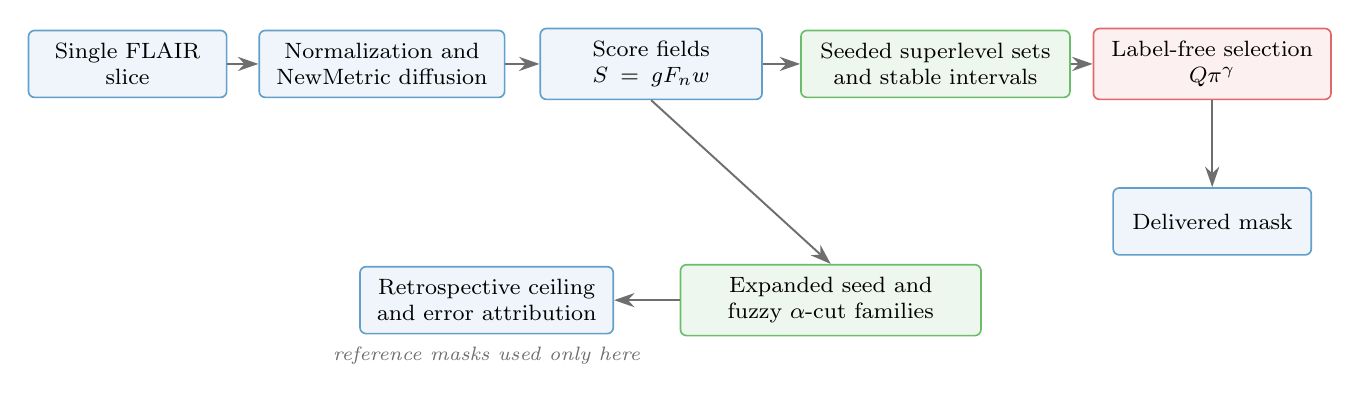
\begin{tikzpicture}[x=0.95mm,y=1mm]
\node[fstep,text width=22mm] (i) at (0,0) {Single FLAIR\\slice};
\node[fstep,text width=28mm] (n) at (34,0) {Normalization and\\NewMetric diffusion};
\node[fstep,text width=25mm] (s) at (70,0) {Score fields\\$S=gF_nw$};
\node[fgen,text width=31mm] (c) at (108,0) {Seeded superlevel sets\\and stable intervals};
\node[fsel,text width=27mm] (q) at (145,0) {Label-free selection\\$Q\pi^\gamma$};
\node[fstep,text width=22mm] (m) at (145,-20) {Delivered mask};
\node[fgen,text width=35mm] (a) at (94,-30) {Expanded seed and fuzzy $\alpha$-cut families};
\node[fstep,text width=29mm] (u) at (48,-30) {Retrospective ceiling\\and error attribution};
\draw[farrow] (i)--(n); \draw[farrow] (n)--(s); \draw[farrow] (s)--(c);
\draw[farrow] (c)--(q); \draw[farrow] (q)--(m);
\draw[farrow] (s.south)--(a.north); \draw[farrow] (a)--(u);
\node[flabel,below=1mm of u] {reference masks used only here};
\end{tikzpicture}
\caption{\textbf{Study method and analytical separation.} The upper sequence
produces the label-free segmentation. Expanded seed and fuzzy $\alpha$-cut
families are evaluated only to measure candidate capacity and attribute errors;
they do not replace the primary delivered mask.}
\label{fig:flow-pipeline}
\end{figure}

\subsection{Conditional Brain-ROI Renormalization}\label{sec:selection}

In skull-intact TCGA images, bright extracranial structures can determine the
normalization maximum and compress intra-brain tumour contrast. A morphological
brain ROI was therefore estimated from the image, with peripheral bright tissue
removed and orbital regions excluded when their dark-centred, approximately
circular and lateral configuration satisfied the predefined anatomical rules.
The score fields and primary candidate family were then reconstructed within this
ROI. Let $M_0$ and $M_1$ denote the masks selected before and after ROI
renormalization, respectively, and let $f_{\mathrm{in}}(M)=|M\cap R|/|M|$. The
ROI-renormalized mask was adopted only if
\begin{equation}
 f_{\mathrm{in}}(M_0)<0.65\quad\text{and}\quad
 f_{\mathrm{in}}(M_1)\ge0.50;
\label{eq:roi-gate-primary}
\end{equation}
otherwise $M_0$ was retained. The condition is inactive for already
skull-stripped images and was therefore not independently validated by the two
external cohorts.

\subsection{Expanded Candidate-Capacity Analysis}\label{sec:saturation-method}

The expanded analysis tested whether a suitable boundary was absent from the
candidate family or present but not recoverable by label-free ranking. In
addition to seeded superlevel-set candidates, four-centre one-dimensional fuzzy
$c$-means~\cite{bezdek1981} was applied to intra-support intensities. The darkest class was
excluded, and connected components of fixed membership $\alpha$-cuts were added
as seed-independent boundary hypotheses. These candidates were used for capacity
measurement, not for the primary delivered segmentation.

Nested seed budgets $s\in\{10,15,20,25,30\}$ and nested $\alpha$-level counts
$a\in\{0,6,11,15,23,39\}$ were evaluated without removing candidates admitted
at smaller budgets. For case $i$,
\begin{equation}
 U_i(s,a)=\max_{M\in\mathcal C_{i,s,a}}D(M,G_i),\qquad
 U(s,a)=\frac{1}{N}\sum_{i=1}^{N}U_i(s,a),
\label{eq:saturation-ceiling}
\end{equation}
where $G_i$ is the reference mask. $U$ is therefore a retrospective
candidate-family ceiling. Practical saturation required the upper bounds of the
paired bootstrap $95\%$ confidence intervals for both final budget increments to
be smaller than the prespecified margin $\varepsilon=0.005$ Dice.

\subsection{Error Decomposition and Evaluation Measures}\label{sec:eval}

For each case, candidate localization was summarized by
$R_{\max}=\max_j|M_j\cap G|/|G|$, and boundary availability by the pool-oracle
Dice $D_{\max}=\max_jD(M_j,G)$. Errors were assigned hierarchically:
$R_{\max}<0.50$ indicated localization failure;
$R_{\max}\ge0.50$ and $D_{\max}<0.70$ indicated boundary-representation failure;
$D_{\max}\ge0.70$ with $D_{\max}-D(\widehat M,G)\ge0.10$ indicated selection
failure; all remaining cases were classified as near-ceiling/successful. These
thresholds are operational diagnostic definitions, not clinical decision limits.

The primary performance measure was Dice, calculated over all cases including
complete misses. Jaccard overlap, sensitivity, precision, the number of zero-Dice
cases, and the numbers exceeding Dice thresholds of 0.50 and 0.70 were secondary
measures. Boundary agreement was characterized by average symmetric surface
distance, 95th-percentile Hausdorff distance, and boundary F1 within two pixels;
distance measures were summarized only when the two masks overlapped
~\cite{taha2015}. Lesion-level
sensitivity, precision and F1 used connected-component matching at
$\operatorname{IoU}\ge0.10$.

Boundary strength was measured in inner and outer bands of the reference contour.
The primary descriptor was the fraction of boundary locations whose NewMetric
gradient magnitude fell below the intra-support median. Additional descriptors
included normal-direction gradient magnitude and sign consistency, inner--outer
ring intensity separation, tumour area and compactness. These quantities used
ground truth only for retrospective error attribution.

\subsection{Statistical Analysis}\label{sec:statistics}

The observational unit was one prespecified axial slice per imaging study.
TCGA-LGG and UCSF-PDGM contributed one study per patient. The 150 BraTS studies
represented 143 unique patients; repeated studies were kept in the same
resampling cluster. Means included zero-Dice cases. Percentile bootstrap $95\%$
confidence intervals used 20,000 resamples. Case-level differences were resampled
for paired comparisons, whereas boundary analyses used patient-clustered
resampling. The corresponding fixed random seeds were 20260715 for primary paired
analyses and 20260723 for cross-cohort boundary analyses.

Paired mean differences were tested with a two-sided Monte Carlo sign-flip test
using 20,000 permutations. The three smoothing comparisons constituted one
family and were adjusted by the Holm procedure. Spearman correlations quantified
the association between boundary descriptors and candidate ceilings; partial
Spearman analyses controlling for area, compactness and ring contrast used 5,000
clustered resamples. The UCSF grade comparison was exploratory and used a
two-sided Mann--Whitney $U$ test, Cliff's $\delta$~\cite{cliff1993} and an independent bootstrap
interval for the mean difference. Parameter sweeps and all TCGA-based parameter
comparisons were treated as developmental rather than confirmatory.

\begin{table}[htbp]\centering
\caption{Fixed parameters of the primary label-free method and the retrospective
capacity analysis.}\label{tab:method-parameters}
\small
\begin{tabular}{lll}
\toprule
Stage & Parameter & Fixed value \\
\midrule
Normalization & Non-background support & $I>0.05$ \\
NewMetric & $\beta_{\mathrm{NM}}$, $\Delta t$, iterations & $5.0$, $0.15$, $3$ \\
Edge field & Gradient and scale & Sobel magnitude; intra-support $P_{95}$ \\
Intensity weighting & Lower bound; softness & $0.28$; $0.05$ \\
Intensity weighting & Upper windows & $0.82$ and $0.97$ \\
Seed localization & FLAIR percentile bands & $[30,88]$ and $[30,98]$ \\
Seed localization & Maximum per window; spacing & $10$; $12$ pixels \\
Region evolution & Threshold range; levels & $S(s)$--$0.20S(s)$; $200$ \\
Region evolution & Area cap; jump ratio & $0.25|B|$; $4$ \\
Stable interval & Relative area tolerance & $0.06$ \\
Candidate eligibility & Minimum area & $\max(40,0.02|B|)$ pixels \\
Selection & Persistence exponent $\gamma$ & $1$ \\
ROI condition & Adoption thresholds & $f_{\mathrm{in}}(M_0)<0.65$, $f_{\mathrm{in}}(M_1)\ge0.50$ \\
Capacity analysis & Seed budgets & $10,15,20,25,30$ per window \\
Capacity analysis & Nested $\alpha$ counts & $0,6,11,15,23,39$ \\
Saturation & Practical Dice margin & $0.005$ \\
\bottomrule
\end{tabular}
\end{table}

\iffalse % Superseded extended Methods retained temporarily for source-level audit.

\subsection{Primary Training-Free Segmentation Method}\label{sec:overview-legacy}

The design principle is not to commit to a single early boundary hypothesis,
but to generate \textbf{many plausible candidates} in an unsupervised manner and
to \textbf{select} the best among them with a label-free quality criterion
(\emph{generate--diversify--select}). The method consists of the following six
steps:

\begin{enumerate}\itemsep1pt
\item \textbf{Normalization and smoothing.} FLAIR intensities are scaled to
$[0,1]$, the brain region is isolated, and the image is smoothed by
edge-preserving diffusion ($\to F_n$).
\item \textbf{Score map.} Each pixel is assigned a score quantifying the
likelihood of lying inside the tumour.
\item \textbf{Seeding.} The most prominent local maxima of the score map are
selected as initial seeds.
\item \textbf{Multi-scale threshold sweeping.} Starting from each seed, the score
threshold is swept from high to low; as the threshold falls, the connected region
containing the seed grows. Every \emph{plateau} over which the area remains stable
during this growth is recorded as a candidate together with its
\emph{persistence}.
\item \textbf{Selection.} The best of all candidates is determined by jointly
evaluating a label-free geometric quality criterion and the plateau persistence.
\item \textbf{Multi-window evaluation.} Steps 1--5 are applied separately with
two intensity windows, one tight and one loose; the final segmentation is chosen
by a window-agnostic arbitration criterion.
\end{enumerate}

The six methodological stages and the complementary candidate-generation
mechanisms are summarized in Figure~\ref{fig:flow-pipeline}:
normalization, with gated brain-ROI renormalization activated only when the gate
conditions are met; edge-preserving NewMetric diffusion producing $F_n$; the score
map built as the product of the edge indicator $g_{nm}$, the smoothed intensity
$F_n$ and the intensity window $w$; and the merged two-channel pool feeding a
single label-free selection.

\begin{figure}[htpb!]\centering
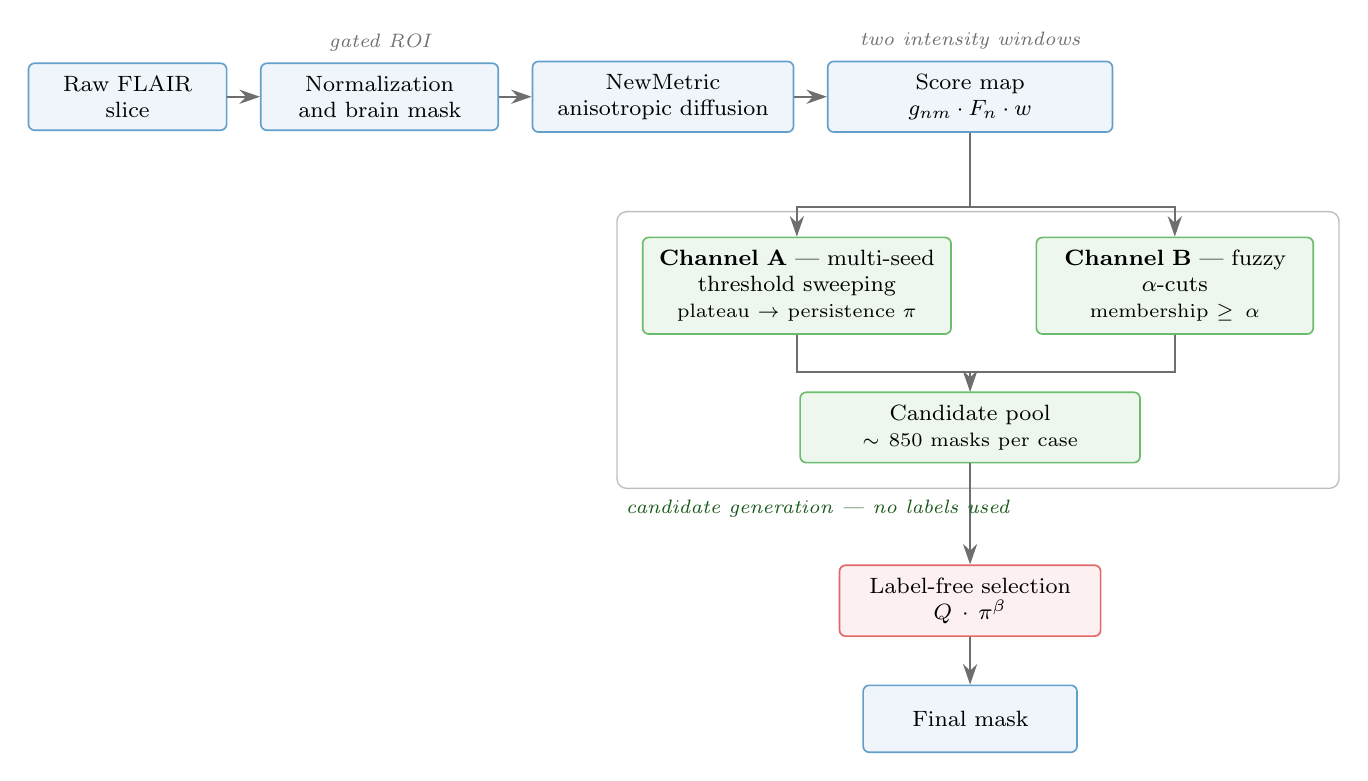
\begin{tikzpicture}[x=1mm, y=1mm]
  % --- top row: construction of the score map ---
  \node[fstep, text width=22mm] (in)    at (  0, 0) {Raw FLAIR\\slice};
  \node[fstep, text width=27mm] (norm)  at ( 32, 0) {Normalization\\and brain mask};
  \node[fstep, text width=30mm] (diff)  at ( 68, 0) {NewMetric\\anisotropic diffusion};
  \node[fstep, text width=33mm] (score) at (107, 0) {Score map\\$g_{nm}\!\cdot\!F_n\!\cdot\!w$};

  % --- two generation channels ---
  \node[fgen, text width=36mm] (sweep) at ( 85,-24)
    {\textbf{Channel A} --- multi-seed\\threshold sweeping\\{\scriptsize plateau $\to$ persistence $\pi$}};
  \node[fgen, text width=32mm] (alpha) at (133,-24)
    {\textbf{Channel B} --- fuzzy\\$\alpha$-cuts\\{\scriptsize membership $\ge\alpha$}};
  \node[fgen, text width=40mm] (pool)  at (107,-42)
    {Candidate pool\\{\scriptsize $\sim\!850$ masks per case}};
  \node[fsel, text width=30mm] (sel)   at (107,-64) {Label-free selection\\$Q\cdot\pi^{\beta}$};
  \node[fstep, text width=24mm] (out)  at (107,-79) {Final mask};

  \draw[farrow] (in) -- (norm);
  \draw[farrow] (norm) -- (diff);
  \draw[farrow] (diff) -- (score);
  \draw[farrow] (score.south) -- (107,-14) -| (sweep.north);
  \draw[farrow] (score.south) -- (107,-14) -| (alpha.north);
  \draw[farrow] (sweep.south) |- (107,-35) -- (pool.north);
  \draw[farrow] (alpha.south) |- (107,-35) -- (pool.north);
  \draw[farrow] (pool) -- (sel);
  \draw[farrow] (sel) -- (out);

  \node[flabel, above=0.8mm of norm] {gated ROI};
  \node[flabel, above=0.8mm of score] {two intensity windows};
  \begin{scope}[on background layer]
    \node[fgroup, fit=(sweep)(alpha)(pool), inner sep=9pt] (genbox) {};
  \end{scope}
  \node[flabel, anchor=north west, text=flowgreen!55!black]
    at ($(genbox.south west)+(0.6mm,-0.8mm)$) {candidate generation --- no labels used};
\end{tikzpicture}
\caption{\textbf{Data flow of the method.} Channel~A (plateau candidates by
multi-seed threshold sweeping) and channel~B (boundary hypotheses from fuzzy
$\alpha$-cuts) feed a shared pool, from which the final mask is selected as
$\arg\max Q\cdot\pi^{\beta}$ with the label-free criterion $Q$. The green frame
marks the generation stage, in which no labels are used.}
\label{fig:flow-pipeline}
\end{figure}

\subsection{Image Normalization and Score-Field Construction}\label{sec:score-setup}

The first methodological stage constructs a score field from the FLAIR image.
This process consists of three steps: normalization and smoothing, computation of
the edge indicator, and formation of the product of the intensity window with the
score.

\paragraph{Normalization and smoothing.} The raw FLAIR $I_{\text{raw}}$ is first
divided by its maximum to bring it into $[0,1]$. The brain region is separated
from the background by the threshold $I > 0.05$, and the intra-brain intensities
are renormalized:
\begin{equation}
I=\frac{I_{\text{raw}}}{\max I_{\text{raw}}},\quad
\mathbf{1}_{\text{brain}}=\{I>0.05\},\quad
I_n=\frac{I}{\max_{\text{brain}} I}.
\label{eq:norm}
\end{equation}
Edge-preserving anisotropic diffusion derived from Finsler metrics (NewMetric;
$\kappa_s=5.0$, $\mathrm{d}t=0.15$, $\text{iter}=3$) is then applied, and the
result is rescaled to $[0,1]$ within the brain to obtain the smoothed field
$F_n$:
\begin{equation}
F_n=\frac{\text{NewMetric}(I)-\min_{\text{brain}}}{\max_{\text{brain}}-\min_{\text{brain}}}.
\label{eq:fn}
\end{equation}
The purpose of this step is to smooth homogeneous regions while preserving tumour
boundaries. No Gaussian smoothing is used in the primary method;
No Gaussian-smoothed result is included in the corrected pure-FLAIR evidence set.

\paragraph{Edge indicator.} The gradient magnitude is computed on the smoothed
$F_n$ with a Sobel kernel, $G=\lVert\nabla F_n\rVert$. The smooth (rational) form
of the Perona--Malik conductance~\cite{peronamalik1990} yields an edge indicator
with a scale $K$ read automatically from the image:
\begin{equation}
g_{nm}=\frac{1}{1+(G/K)^2},\qquad K=P_{95}\big(G\,;\,\mathbf{1}_{\text{brain}}\big).
\label{eq:gnm}
\end{equation}
$g_{nm}\approx 1$ indicates a homogeneous (traversable) region, whereas
$g_{nm}\to 0$ indicates a sharp edge (a wall).

\paragraph{Intensity window and score map.} Candidate tumour pixels are filtered
by a two-sided sigmoidal band-pass:
\begin{equation}
\mathrm{win}(I_n)=
\frac{1}{1+e^{-(I_n-\tau_{\text{lo}})/s_w}}
\times
\frac{1}{1+e^{\,(I_n-\tau_{\text{hi}})/s_w}},
\label{eq:win}
\end{equation}
where $\tau_{\text{lo}}=0.28$ is the lower threshold, $s_w=0.05$ the transition
smoothness, and $\tau_{\text{hi}}$ the upper bound that forms the core of the
multi-window architecture. The lower threshold $\tau_{\text{lo}}$ is positioned so
as to leave the cerebrospinal fluid and background levels of the normalized
intensity outside the candidate tumour band; its role differs from that of the
upper bound, in that it determines the exclusion of non-candidates rather than the
brightness range of the tumour. The transition smoothness $s_w$ is the single
parameter that makes the window a differentiable weight rather than a binary
indicator: in the limit $s_w\to0$ the window reduces to a hard threshold and the
score becomes discontinuous at pixels near it. Both values were determined on the
TCGA-LGG development set and frozen unchanged across all three cohorts; the
sensitivity of performance along these axes is not re-estimated in the corrected
pure-FLAIR audit. The score map is built as the product of three pieces
of evidence (edge traversability, brightness, intensity band) with the brain mask:
\begin{equation}
\mathrm{score}=g_{nm}\cdot F_n\cdot \mathbf{1}_{\text{brain}}\cdot \mathrm{win}.
\label{eq:score}
\end{equation}
The product is a deliberate choice: a pixel receives a high score only when it
satisfies all three conditions at once; if any one of them is low, the score
collapses. For window-agnostic selection, an arbitration criterion excluding the
window term is also defined:
\begin{equation}
\mathrm{eval}=g_{nm}\cdot F_n\cdot \mathbf{1}_{\text{brain}}.
\label{eq:eval}
\end{equation}

\subsection{Rationale for Multiplicative Evidence Pooling}\label{sec:score-rationale}

The choice of a \emph{product} rather than a sum or a weighted average in
Eq.~\eqref{eq:score} is not incidental; it is forced by three mutually
reinforcing readings --- probabilistic, information-theoretic and algebraic ---
that single out the product and, critically, rule out the sum. Each of the three
factors is a membership in $[0,1]$: $\mu_1=g_{nm}$ (edge traversability),
$\mu_2=F_n$ (diffused brightness), $\mu_3=\mathrm{win}$ (intensity band).
Restricted to the brain, the score is written as $S=\prod_{k} \mu_k$.

\paragraph{Probabilistic reading: naive-Bayes pooling.} Let $y\in\{0,1\}$ be the
latent intra-tumour indicator at a pixel and let $e_1,e_2,e_3$ be the pieces of
evidence underlying the three factors. Under the assumption that the evidence is
conditionally independent given the class --- the naive-Bayes assumption --- the
posterior odds factorize:
\begin{equation}
\frac{P(y{=}1\mid e_1,e_2,e_3)}{P(y{=}0\mid e_1,e_2,e_3)}
=\frac{P(y{=}1)}{P(y{=}0)}\;\prod_{k}\frac{p(e_k\mid y{=}1)}{p(e_k\mid y{=}0)},
\label{eq:naivebayes}
\end{equation}
so that, upon taking logarithms,
\begin{equation}
\operatorname{logit}P(y{=}1\mid e)=\operatorname{logit}P(y{=}1)+\sum_{k}\log \mathrm{LR}_k(e_k),
\qquad \mathrm{LR}_k=\frac{p(e_k\mid y{=}1)}{p(e_k\mid y{=}0)}.
\label{eq:logit}
\end{equation}
If each membership $\mu_k$ is interpreted as a monotone surrogate for the
per-evidence likelihood ratio $\mathrm{LR}_k$, then the log-score
$\log S=\sum_k \log \mu_k$ is the naive-Bayes log-posterior-odds up to a shift by
the class prior. Thresholding $S$ is then rank-equivalent to thresholding the
posterior. We emphasize that the $\mu_k$ are handcrafted rather than calibrated
likelihoods, so that~\eqref{eq:logit} is an interpretive correspondence rather
than an exact identity; its value is that it fixes the \emph{pooling rule}
(additive in log space, hence multiplicative in $S$) independently of any weights
--- decisive in a label-free regime where weights cannot be fitted.

\paragraph{Information-theoretic reading: additivity of surprisal.} Equivalently,
$-\log S=\sum_k(-\log\mu_k)$ is a sum of Shannon surprisals. Each term
$-\log\mu_k$ is the information content of the $k$-th piece of evidence, and the
product rule is precisely the statement that information from independent sources
adds. The total surprisal of a pixel is small only when no single piece of
evidence is individually surprising under the intra-tumour hypothesis; a single
surprising piece of evidence (a bright out-of-band pixel, an edge wall) adds an
unbounded penalty, since $-\log\mu_k\to\infty$ as $\mu_k\to0$.

\paragraph{Algebraic reading: the product is the unique admissible pooling.} The
pooling rule can be characterized axiomatically. A binary operation
$T:[0,1]^2\to[0,1]$ that is continuous, commutative, associative, non-decreasing
in each argument and satisfies the unit boundary condition $T(a,1)=a$ is a
\emph{triangular norm} (t-norm). The following singles out the product among all
such rules.

\begin{proposition}\label{prop:tnorm}
Let $T$ be a continuous Archimedean t-norm --- that is, $T(a,a)<a$ for every
$a\in(0,1)$. Then there exists a continuous, strictly decreasing generator
$\varphi:[0,1]\to[0,\infty]$, unique up to a positive scalar, such that
\begin{equation}
T(a,b)=\varphi^{-1}\!\big(\varphi(a)+\varphi(b)\big).
\label{eq:aczel}
\end{equation}
Moreover, if $T$ is \emph{strict} (strictly increasing on $(0,1]^2$), then
$\varphi(0)=\infty$, so that $T$ has the annihilator property $T(0,b)=0$ for every
$b$. The product $T(a,b)=ab$ is the strict Archimedean t-norm with generator
$\varphi(a)=-\log a$, and it is the unique such t-norm for which the induced
evidence measure $\varphi(\mu_k)$ is the Shannon surprisal $-\log\mu_k$.
\end{proposition}

\begin{proof}
The representation~\eqref{eq:aczel} is the Aczél representation theorem for
continuous Archimedean t-norms; $\varphi$ is the additive generator and its
uniqueness up to positive scaling is standard~\cite{bao2000}. Strictness is
equivalent to $\varphi(0)=\infty$, whence
$T(0,b)=\varphi^{-1}(\varphi(0)+\varphi(b))=\varphi^{-1}(\infty)=0$. Substituting
$\varphi=-\log$ into~\eqref{eq:aczel} gives $\varphi^{-1}(u)=e^{-u}$ and
$T(a,b)=e^{-(-\log a-\log b)}=ab$. Fixing the generator to be the surprisal
$-\log$ (equivalently, requiring log-additive evidence pooling as
in~\eqref{eq:logit}) determines $T$ uniquely as the product, up to the scalar
freedom in $\varphi$, which cancels under $\varphi^{-1}$.
\end{proof}

Two design requirements of the score are thus met simultaneously, and only by the
product: log-additive pooling of independent evidence (the generator is the
surprisal) and the \emph{veto} (annihilator) property
$\mu_k\to0\Rightarrow S\to0$. The veto is exactly what a sum lacks: for
$S_{\mathrm{sum}}=\sum_k\mu_k$ a single dominant factor masks the output of the
others (an OR-like behaviour), so that a bright vessel with
$g_{nm}\approx1,\,F_n\approx1$ but $\mathrm{win}\approx0$ still receives a high
score --- the dominant empirical failure mode that the pipeline must suppress. The
product annihilates such a pixel regardless of its other factors.

\paragraph{Geometric reading.} The three factors also admit a direct geometric
interpretation that distinguishes the stages defined in Appendix~\ref{sec:theory}: $g_{nm}$ is a
Euclidean-gradient Perona--Malik conductance evaluated after NewMetric --- a
membership answering the question ``is this pixel in a homogeneous, geometrically
traversable region?''; $F_n$ is the diffused feature coordinate of the
immersion~\eqref{eq:immersion}; and $\mathrm{win}$ is a band-pass on intensity.
The score is thus the fuzzy intersection of a geometric-traversability set, a
brightness set and an intensity-band set.

\paragraph{Window-agnostic arbiter.} Dropping the window factor leaves
$\mathrm{eval}=g_{nm}\cdot F_n\cdot\mathbf{1}_{\text{brain}}$
(Eq.~\ref{eq:eval}). Because the tight and loose windows
(Section~\ref{sec:selection}) place their candidates on different score scales, a
cross-window comparison requires a window-agnostic quality; $\mathrm{eval}$ is
exactly the sub-product that survives removing the intensity-band evidence, and
therefore serves as a common arbiter that favours the grade assumption of neither
window.

The individual appearance of the factors constituting the score map is shown in
Figure~\ref{fig:score-components}.

\begin{figure}[htbp!]\centering

\includegraphics[width=0.96\linewidth]{fig_score_components_tcga.png}
\caption{\textbf{Components of the score map.} The score is the product of three
independent pieces of evidence: $g_{nm}$ (edge traversability), $F_n$ (diffused
brightness) and win (intensity window). The product ensures that a pixel receives
a high score only when it satisfies all three conditions at once. The green
contour shows the ground truth.}
\label{fig:score-components}
\end{figure}

\subsection{Candidate Generation}\label{sec:candidates}

Candidate masks are generated by a multi-seed, multi-scale threshold sweep over
the score map. This process consists of two steps: seed selection and threshold
sweeping with persistence tracking.

\paragraph{Seed selection.} The score map is restricted to a FLAIR intensity
band: $\text{band}=\{p_{30}\le I_n\le p_{\text{band}}\}\cap\mathbf{1}_{\text{brain}}$.
The local maxima of this band are selected as seeds, separated by at least
$d_{\min}=12$ pixels and numbering at most $N_s=10$ (here $N_s$ is the seed
budget; it should not be confused with the edge scale $K$ of
Eq.~\eqref{eq:gnm}). The band removes the dimmest $30\%$ (healthy tissue) and the
brightest few percent (vessels/artefacts), leaving a ``bright but not extreme''
band. Multiple seeds are used because it is not known in advance which bright
structure is the tumour; all plausible starting points are seeded and the correct
one is left to the selection stage.

\paragraph{Threshold sweeping and persistence tracking.} Starting from each seed,
the score threshold is swept from high to low. At each threshold level, the
connected component of $\{\mathrm{score}\ge t\}\cap\mathbf{1}_{\text{brain}}$
containing the seed (a superlevel set) is the current candidate. Thresholds are
swept in $200$ steps, $t\in\text{linspace}(s_v, 0.20\,s_v, 200)$. Let $a_j$ be the
region area at step $j$ and $\Delta_j=a_j-a_{j-1}$ the successive increment. The
jump and acceleration criteria are applied only after the region has reached a
\emph{stable-area threshold} of $n_{\min}=\max(40,\;0.02\,|\Omega_{\text{brain}}|)$
pixels, the purpose being not to mistake the natural growth of a region that is
still only a few pixels wide for leakage. Growth stops when one of the following
stopping criteria is met: (i)~edge wall --- the mean $g_{nm}$ on the candidate
boundary falls below $0.08$; (ii)~area cap --- the region exceeds $25\%$ of the
brain area; (iii)~sudden jump --- $a_j>4\,a_{j-1}$ while $a_{j-1}\ge n_{\min}$;
(iv)~acceleration --- $\Delta_j>2.5\,\Delta_{j-1}$ and
$\Delta_{j-1}>2.5\,\Delta_{j-2}+1$ while $a_{j-1}\ge n_{\min}$ and the last three
increments are positive. Threshold levels at which the area remains below $5$
pixels are passed over without producing a candidate.

As the threshold decreases the region grows; the stable intervals (plateaus) over
which the area remains constant are recorded as candidate masks. Plateau tracking
begins once the region reaches $30$ pixels; a plateau is defined by the area not
exceeding $(1+\varepsilon)$ times its initial value ($\varepsilon=0.06$) over
successive steps. This tolerance determines how strict the definition of stability
is: in the limit $\varepsilon\to0$ only intervals over which the area is exactly
constant count as plateaus, and because of discretization noise most seeds then
produce no candidate at all; a large $\varepsilon$, conversely, admits regions
that have already begun to leak and renders the persistence measure meaningless.
The value was determined on the TCGA-LGG development set and frozen across all
cohorts; the corrected audit keeps $\varepsilon$ frozen. Each
candidate carries a \emph{persistence} value $\pi$ measuring how many steps the
plateau lasted along the threshold range. This value quantifies the height of the
plateau wall in the score-field landscape --- how far the threshold can fall
before the region merges with a neighbour. The question ``how far should growth
continue'' thus ceases to be a parameter and becomes a selection problem.

\paragraph{Direct fuzzy $\alpha$-cut candidates.} In a fuzzy set each pixel is
described by a membership degree $u(x)\in[0,1]$; the \emph{$\alpha$-cut} of that
set at level $\alpha$ is the crisp set of pixels whose membership is at least
$\alpha$:\ $A_\alpha=\{x:u(x)\ge\alpha\}$. As $\alpha$ increases, $A_\alpha$
shrinks and a nested family of sets arises; by the decomposition principle of
fuzzy set theory this family represents the fuzzy set in
full~\cite{bezdek1981}. In segmentation terms this means that, instead of
selecting a single threshold, one obtains a family of nested \emph{boundary
hypotheses} along the $\alpha$ axis, and the decision as to which level is correct
is deferred to the selection stage. This is the intensity-axis counterpart of the
\emph{generate--diversify--select} principle of the study.\par The rationale for
using the two channels together is that they fail in different ways. Threshold
sweeping is \emph{seed-dependent} and \emph{connectivity-constrained}: if a seed
does not fall on the tumour, or if the tumour is connected to neighbouring tissue
through a low-contrast isthmus, no threshold level can return the correct region
as a single component. $\alpha$-cuts, by contrast, operate \emph{without seeds}
and \emph{globally}: because the membership map is estimated from the whole image,
a lesion missed by seeding may still emerge at a suitable $\alpha$ level. On the
other hand, $\alpha$-cuts do not use the score topology; plateau stability and
edge-wall information exist only in the traversal channel. The two channels are
therefore not substitutes for one another: one produces the boundary hypotheses of
intensity membership, the other those of score topology, and they merge in the
pool. Threshold sweeping produces the score components reachable from a seed,
while fuzzy intensity membership supplies this complementary boundary family. A
four-centre one-dimensional fuzzy $c$-means~\cite{bezdek1981} is applied to the
intra-brain $I_n$ values; the darkest cluster is excluded, and for the remaining
membership maps $u_k(x)$ the connected components of the superlevel sets
$\{x:u_k(x)\ge\alpha\}$ that satisfy the area constraint are added directly as
candidates. This channel does not replace the score-topology superlevel-set sweep: it separates the
seeding from the traversal logic and merges, for the same image, the
complementary boundary hypotheses of intensity membership and score topology in
the pool. No Gaussian or median pre-smoothing is used. The computation--coverage
balanced configuration proposed here uses $15$ standard seeds per window and six
$\alpha$ levels ($0.35,0.45,\ldots,0.85$); $30$ seeds and $39$ nested $\alpha$
levels constitute the research budget used solely to characterize the saturation
ceiling of the candidate family. The concrete effect of the channel on a single
case is shown in Figure~\ref{fig:alpha-cut}: as $\alpha$ rises the cut sets shrink
and a nested family of boundary hypotheses forms, and which level is correct is not
decided at the generation stage but left to selection. Under the corrected
implementation,
the illustrated case demonstrates convergent but non-identical hypotheses: both
channels represent the tumour accurately, while arriving at their boundaries by
different constructions.

\begin{figure}[htpb!]\centering

\includegraphics[width=0.99\linewidth]{fig_alpha_cut_illustration.png}
\caption{\textbf{Effect of the $\alpha$-cut channel on a single case}
(TCGA\_DU\_6400, cropped to the brain). (A)~Raw FLAIR with the ground-truth
boundary (green). (B)~Fuzzy $c$-means membership $u_2(x)$ of the tumour's cluster
(lighter~$=$~higher). (C)~Candidate components from cuts of that map,
colour-coded by $\alpha$. (D)~Best candidate per channel: $\alpha$-cut $0.959$
(blue) against seeded sweeping $0.962$ (red dashed). Dice values are retrospective,
not inference performance.}
\label{fig:alpha-cut}
\end{figure}


\subsection{Topological Basis of Persistence Selection}\label{sec:persistence-theory}

The persistence value $\pi$ attached to each candidate is not an arbitrary
stability heuristic; it is the $0$-dimensional persistence of the seed component
under a superlevel-set filtration, and this identification gives both a precise
meaning to the plateau and a formal explanation of why $\pi$ transfers across
populations while absolute-intensity signals do not.

\paragraph{Superlevel-set filtration.} For a threshold $t$, let
$X_t=\{x\in\Omega_{\text{brain}}:S(x)\ge t\}$ be the superlevel set of the score.
As $t$ decreases these sets are nested,
\begin{equation}
t_1\ge t_2\;\Longrightarrow\; X_{t_1}\subseteq X_{t_2},
\label{eq:filtration}
\end{equation}
forming the superlevel filtration of $S$. The candidate at level $t$ is the
connected component $C_t(s)\subseteq X_t$ containing the seed $s$. Treating $S$ as
a Morse function with distinct critical values~\cite{milnor1963}, the homotopy
type of $X_t$ changes only as $t$ crosses a critical value: at each local maximum
a new connected component (a $0$-cycle) is born, and two components merge at a
saddle.

\paragraph{Merge tree, elder rule and persistence diagram.} The birth--death
history of the components is organized by the \emph{merge tree} $\mathcal{T}$: its
leaves are local maxima (births), its internal nodes are merge saddles, and its
descending edges track each component until it merges. When two components with
birth values $b_1>b_2$ meet at a saddle of value $d$, the \emph{elder rule} of
persistent homology dictates that the younger class (the smaller birth $b_2$) dies
and the elder one ($b_1$) survives; in homological terms the map
$H_0(X_{d+\epsilon})\to H_0(X_{d-\epsilon})$ has a one-dimensional kernel spanned
by the younger generator~\cite{edelsbrunner2002}. The dying class contributes a
point $(b_2,d)$ to the $0$-dimensional persistence diagram,
\begin{equation}
\mathrm{Dgm}_0(S)=\{(b_i,d_i)\}_i,\qquad b_i>d_i,
\label{eq:dgm}
\end{equation}
with persistence $\mathrm{pers}_i=b_i-d_i$.

\paragraph{The plateau as the stable interval of the seed component.} The area of
the seed component, $A(t)=|C_t(s)|$, is a non-decreasing staircase as $t$
decreases: it is constant over the intervals in which lowering the threshold adds
no pixels --- the seed component is walled off by a steep score drop --- and jumps
at the saddles where $C_t(s)$ swallows a neighbour or pierces a low barrier (a
leak). A \emph{plateau} is a maximal interval $[t_-,t_+]$ over which the area
remains stable, with $A(t)\le(1+\varepsilon)A(t_+)$ for all $t\in[t_-,t_+]$
(Section~\ref{sec:candidates}, $\varepsilon=0.06$), and the recorded persistence
is its threshold width,
\begin{equation}
\pi=t_+-t_-,
\label{eq:pi-def}
\end{equation}
the vertical margin over which the seed component survives before its next merge.
Equivalently, $\pi$ measures the depth of the score barrier --- the moat --- that
separates the candidate from the neighbouring structure with which it will merge;
a wide, steep-walled tumour occupies a long plateau, whereas a candidate bounded
by a shallow barrier merges almost immediately and carries a small $\pi$.

\iffalse % Legacy backend visualization; excluded until regenerated under the corrected operator.
\begin{figure}[htbp!]\centering
\includegraphics[width=0.98\linewidth]{fig_persistence_plateau.png}
\caption{\textbf{Topological persistence of the seed component.} (a)~Area $A(t)$ of
the seed component as the score threshold $t$ falls: stable over a wide interval
(amber plateau, persistence $\pi=t_+-t_-$), then jumping at the merge/leak
threshold (red dashed) where the component swallows neighbouring tissue.
(b)~Representative mask taken at the low-threshold end of the plateau (amber)
against the expert ground truth (green); the seed is marked with a cyan cross.}
\label{fig:persistence}
\end{figure}
\fi

\paragraph{Monotone invariance and population transfer.} The decisive property of
persistence is its invariance under reparameterization of the score.

\begin{proposition}[Monotone invariance of the persistence ordering]\label{prop:monotone}
Let $\phi:\mathbb{R}\to\mathbb{R}$ be strictly increasing and let $S'=\phi\circ S$
be any per-image monotone renormalization of the score. Then the superlevel
filtrations of $S$ and $S'$ coincide up to a relabelling of thresholds, and the
induced merge trees, the birth--death ordering and the ordering of candidates by
persistence are identical.
\end{proposition}

\begin{proof}
For every $t$, since $\phi$ is strictly increasing and hence order-preserving,
$X'_{\phi(t)}=\{x:\phi(S(x))\ge\phi(t)\}=\{x:S(x)\ge t\}=X_t$. The nested family
in~\eqref{eq:filtration} is therefore mapped to itself under the relabelling
$t\mapsto\phi(t)$; the sequence of inclusions --- and with it every birth, death
and merge event, and the entire merge tree $\mathcal{T}$ --- is preserved. Only
the numerical threshold labels change. In particular the order in which candidates
reach their merge saddles, and hence their ranking by plateau width, is unchanged.
\end{proof}

Proposition~\ref{prop:monotone} is the formal reason why $\pi$ is the only
selection signal that transfers across populations. Absolute-intensity statistics
(mean brightness, inside/outside contrast) are not monotone-invariant: they shift
with the intensity scale of the cohort, so a threshold calibrated on lower-grade
gliomas mis-ranks high-grade candidates and vice versa. The persistence ordering,
being a property of the superlevel topology alone, is blind to any per-image
monotone rescaling of $S$ and therefore behaves consistently across low-contrast
(LGG) and high-contrast (HGG) regimes. (We record $\pi$ as the raw interval length
$t_+-t_-$; under a non-linear $\phi$ this is invariant in \emph{ordering} but not
in \emph{value}. Since selection uses only $\arg\max$, invariance of the ordering
suffices.)

\paragraph{Stability.} Persistence further carries a robustness guarantee that
raw-score selection lacks. By the stability theorem of Cohen-Steiner, Edelsbrunner
and Harer~\cite{cohensteiner2007}, the persistence diagrams of two score fields
satisfy
\begin{equation}
d_B\big(\mathrm{Dgm}(S),\mathrm{Dgm}(S')\big)\le\lVert S-S'\rVert_\infty,
\label{eq:stability}
\end{equation}
where $d_B$ is the bottleneck distance. A feature of persistence $p$ is preserved
as a matchable feature under perturbations of sup-norm smaller than $p$. This
stability result justifies why long plateaus are more robust to small score
perturbations than short ones; it does not by itself guarantee that a long plateau
belongs to the tumour. While the edge-preserving diffusion of
Appendix~\ref{sec:theory} suppresses high-frequency variation, the persistence
criterion quantifies the continuity of candidates along the threshold; tumour
specificity must be assessed empirically in addition.

\paragraph{Level-dependence of the signal.} Finally, the topological reading
explains the empirically observed two-level behaviour. Within a single slice all
candidates share one filtration, so their persistences are comparable and $\pi$ is
a valid relative barrier measure. Across slices, by contrast, each slice induces
its own filtration and merge tree on an incomparable threshold scale; ranking
slices by $\pi$ would compare persistences drawn from different landscapes, which
the theory does not permit. The topological reading therefore yields only the
following asymmetric prediction: $\pi$ is \emph{invalid} across slices, whereas it
is well defined within a slice. Being valid within a slice does not make it useful
for accuracy, and the measurements show that it is not --- the contribution of the
within-slice persistence weight to mean Dice is not statistically supported
(Section~\ref{sec:stability}), and in the integrated pool $\pi$ was observed not to
be a reliable within-case candidate ranker. A quantitative analysis of this
behaviour is outside the scope of this study.

\subsection{Label-Free Candidate Selection and Conditional ROI Correction}\label{sec:selection}

Two mechanisms are used jointly to select the best mask from the candidate pool
without accessing ground truth during fixed-slice inference: a geometric quality
criterion and a persistence weight. In addition, the multi-window architecture
resolves the grade-dependent window problem, and gated brain-ROI renormalization
resolves a skull-induced normalization artefact.

\paragraph{Geometric quality criterion.} For each candidate mask $M$ a quality
value is computed as the product of four label-free attributes:
\begin{equation}
Q(M)=A\cdot \bar{s}\cdot \mathrm{cp}\cdot \mathrm{sol},
\label{eq:quality}
\end{equation}
where $A=|M|$ is the area, $\bar{s}$ the mean score inside the mask,
$\mathrm{cp}=4\pi A/P^2$ the isoperimetric compactness and
$\mathrm{sol}=A/A_{\text{hull}}$ the solidity (ratio to the convex hull). The
product ensures that a single failing attribute eliminates the candidate.

\paragraph{Persistence weight.} The static quality criterion looks at the frozen
geometry of the candidate, whereas the threshold sweep also attaches a persistence
value $\pi(M)$ to each candidate. A genuine tumour occupies a wide, steep-walled
plateau in the score-field landscape; the region does not grow even though the
threshold varies over a wide interval. To bring this dynamic evidence into the
selection, the quality is weighted by a power of the persistence:
\begin{equation}
\hat M=\arg\max_{M\in\text{pool}}\; Q(M)\cdot \pi(M)^{\beta},\qquad \beta=1.
\label{eq:select}
\end{equation}
$\beta$ was chosen on the development set alone: among
$\beta\in\{0,\tfrac12,1,2\}$, $\beta=1$ gave the best result. Persistence is the
only population-independent signal among those tested --- it helps in the same
direction for both low-contrast and sharply bounded tumours.

\paragraph{Multi-window architecture.} The optimal upper bound
$\tau_{\text{hi}}$ of the candidate tumour window depends systematically on tumour
grade: lower-grade gliomas require a tight window ($\tau_{\text{hi}}=0.82$),
high-grade gliomas a loose one ($\tau_{\text{hi}}=0.97$). A single fixed threshold
inevitably sacrifices one sub-population. The method is therefore applied
separately with two windows, one tight and one loose:
\begin{equation}
(\tau_{\text{hi}},\,p_{\text{band}})\in\{(0.82,\,p_{88}),\;(0.97,\,p_{98})\}.
\label{eq:windows}
\end{equation}
The candidates of the two windows merge into a single pool, and the final mask is
selected by the quality read from the window-agnostic $\mathrm{eval}$ field
(Eq.~\ref{eq:eval}). The correct window --- and implicitly the correct grade
assumption --- is thus chosen per case without using any dataset-level indicator.

\paragraph{Gated brain-ROI renormalization.} A portion of the complete failures
was shown to arise not from genuine isointensity but from a skull-induced
normalization artefact. The brain mask $\{I_n>0.05\}$ is in fact a head mask
(including skull and scalp); since intensity normalization is performed over this
mask, the bright skull sets the normalization ceiling and the low-contrast LGG
tumour is relatively compressed. To remove this artefact, the true intra-brain
region is extracted from the raw slice by intensity thresholding + morphology +
largest connected component + hole filling, and all fields are renormalized; the
bright rim is erased only within a peripheral band. In a minority of slices the
eyeball and the surrounding orbital fat are likewise locally hyperintense, as the
skull is, and may remain inside the ROI without being caught by the
peripheral-band rule; in that case the same normalization-ceiling problem recurs
in the orbital region. To remove it, a region is detected as an eyeball if it has
a dark interior ($I<p_{25}$), is circular ($4\pi A/P^2>0.45$), lies anteriorly (in
the upper $42\%$ of the ROI) and is far from the midline (lateral; this condition
excludes the ventricles); the eye, its symmetric mirror and the surrounding
orbital fat (a $13$-pixel dilation) are then additionally removed from the ROI. If
no eye is detected (mid-slices, already skull-stripped inputs) this step does not
engage and the ROI is unchanged. Once all fields are renormalized over the final
ROI, the skull/orbit ceiling is lifted and the compressed tumour opens up.

This correction is applied conditionally. Let $M_0$ be the currently selected
mask, $M_1$ the selection reconstructed over the ROI, and
$f_{\text{in}}(M)=|M\cap R|/|M|$ the intra-ROI fraction of a mask. The ROI result
$M_1$ is adopted only when $f_{\text{in}}(M_0) < 0.65$ and
$f_{\text{in}}(M_1) \ge 0.5$; otherwise $M_0$ is retained. This condition
activates on the minority of cases carrying a skull/orbit-distractor signature and,
by construction, never triggers on already skull-stripped inputs.

\subsection{Evaluation Measures and Error Decomposition}\label{sec:eval}

Segmentation performance is evaluated with a set of metrics grouped into three
categories: overlap, boundary and lesion level. This multi-metric reporting
approach aims to prevent a single summary number from concealing different
dimensions of performance; the performance distributions of unsupervised
segmentation are often bimodal --- the method either produces a good mask or fails
completely --- so that averaging alone can be misleading.

\paragraph{Overlap metrics.} The volumetric overlap between the prediction
$\hat M$ and the expert ground truth $M_{\mathrm{gt}}$ is measured by the Dice
coefficient:
\begin{equation}
\text{Dice}(\hat M,M_{\mathrm{gt}})=\frac{2\,|\hat M\cap M_{\mathrm{gt}}|}{|\hat M|+|M_{\mathrm{gt}}|}.
\label{eq:dice}
\end{equation}
Dice ranges from $0$ (no overlap) to $1$ (perfect overlap) and is sensitive both to
under-detection and to over-growth. The following additional set-level overlap
metrics are reported. \textbf{Mean(all)} --- the all-case mean including zero-Dice
cases; the most conservative summary and directly comparable with external
methods. \textbf{Mean(nz)} --- the mean over non-zero cases only, reflecting the
overlap quality where the method does detect a tumour. \textbf{D$>$0.5} and
\textbf{D$>$0.7} --- the numbers of cases exceeding the clinical-acceptance and
good-segmentation thresholds. \textbf{Zero} --- the number of complete failures
(Dice$=0$): cases in which the finally selected mask has no overlap at all with
the ground truth. The Jaccard coefficient
($\mathrm{Jaccard}=\mathrm{Dice}/(2-\mathrm{Dice})$) and pixel-level Sensitivity
($\mathrm{TP}/(\mathrm{TP}+\mathrm{FN})$) and Precision
($\mathrm{TP}/(\mathrm{TP}+\mathrm{FP})$) are also reported, where
$\mathrm{TP}=|\hat M\cap M_{\mathrm{gt}}|$,
$\mathrm{FP}=|\hat M\setminus M_{\mathrm{gt}}|$ and
$\mathrm{FN}=|M_{\mathrm{gt}}\setminus \hat M|$. Sensitivity gives how much of the
tumour is captured and Precision how much of the prediction is genuinely tumour;
the relation between the two reveals whether the method tends to over-grow (low
precision) or under-grow (low sensitivity).

\paragraph{Boundary and surface metrics.} Overlap metrics show whether the region
was captured correctly but say nothing directly about boundary accuracy. Distances
between the predicted and ground-truth boundary pixel sets ($\partial\hat M$ and
$\partial M_{\mathrm{gt}}$) are therefore also measured. \textbf{ASSD} (average
symmetric surface distance)~\cite{taha2015} is the mean distance between the two
boundaries:
\begin{equation}
\mathrm{ASSD}=\frac{\sum_{p\in\partial\hat M} d(p,\partial M_{\mathrm{gt}})
+\sum_{q\in\partial M_{\mathrm{gt}}} d(q,\partial\hat M)}
{|\partial\hat M|+|\partial M_{\mathrm{gt}}|},
\label{eq:assd}
\end{equation}
where $d(p,S)=\min_{q\in S}\lVert p-q\rVert$ is the shortest distance from a point
to a set. \textbf{HD$_{95}$} is the $95$th percentile of the same symmetric
distance set and provides a Hausdorff distance robust to
outliers~\cite{taha2015}. \textbf{BoundaryF1@$2$px} is the F1 score of boundary
sensitivity and boundary precision, built from the fractions of boundary pixels
matched within $2$ pixels of the opposing boundary. Boundary metrics are in pixel
units (BraTS being $1\,\text{mm}^3$ isotropic, px$\approx$mm) and are computed
only on overlapping (Dice$>0$) cases; for complete misses the boundary is
undefined, and such cases are already counted under Dice and Zero. The purpose of
these metrics is to quantify how precisely the method draws the boundary even when
it finds the correct region.

\paragraph{Lesion-level metrics.} The connected components (separate lesions) of
$\hat M$ and $M_{\mathrm{gt}}$ are matched if their IoU is $\ge 0.10$. A matched
predicted component counts as a true-positive lesion, an unmatched prediction as a
false positive and an unmatched ground-truth component as a false negative;
lesion-level Sensitivity, Precision and F1 are computed from these counts.
Independently of pixel overlap, this metric answers the question ``how many tumour
foci were detected/missed'' and exposes detection failures that pixel Dice may
conceal in multifocal cases. Lesion-level metrics are computed on all cases.

\paragraph{Retrospective localization--boundary--selection (LBS) analysis.} A
hierarchical diagnostic, in which ground truth is used solely for error
attribution, was applied to the frozen candidate set of the primary method. The
localization criterion is the maximum, over the candidates of a case, of the
fraction of the true tumour captured,
$R_{\max}=\max_j |M_j\cap M_{\mathrm{gt}}|/|M_{\mathrm{gt}}|$. The operational
thresholds were fixed before the analysis: if $R_{\max}<0.50$ the case is a
\emph{localization failure}; if $R_{\max}\ge0.50$ but the pool-oracle Dice is
$<0.70$, a \emph{boundary-representation failure}; if the oracle Dice is $\ge0.70$
but the oracle-minus-selected Dice difference is $\ge0.10$, a \emph{selection
failure}; the remaining cases are classified as \emph{near-ceiling/successful}.
These thresholds are not clinical decision boundaries but diagnostic thresholds
that separate error stages which would otherwise be conflated.
Their descriptive robustness was examined in a complete $3\times3\times3$ grid:
$R_{\max}\in\{0.40,0.50,0.60\}$, oracle Dice
$\in\{0.60,0.70,0.80\}$, and oracle--selected gap
$\in\{0.05,0.10,0.15\}$. This analysis changes only the retrospective error
labels; it does not change any predicted mask.

Boundary geometry was characterized by the NewMetric gradient magnitude in a
one-pixel inner/outer band of the ground-truth contour; the weak-boundary fraction
falling below the intra-brain median gradient; the normal-directional gradient
magnitude and sign consistency; the intensity separation of three-pixel
inner/outer rings; and the ground-truth compactness. The primary feature and the
thresholds were frozen after the TCGA analysis and applied unchanged to UCSF-PDGM
and BraTS~2023. The primary Spearman association in each cohort is reported with a
fixed seed of $20260723$ and $20\,000$ patient-clustered bootstrap resamples; the
partial-Spearman sensitivity analysis controlling for area, compactness and ring
contrast is reported with $5\,000$ resamples. The resampling unit is the patient;
the $150$ studies in BraTS~2023 belong to $143$ unique patients, and repeated
studies of the same patient were kept together in every bootstrap draw. The UCSF
grade 2 and grade 3 subgroups were examined separately, and cross-cohort effect
differences were computed from independent bootstrap distributions. The Fisher-$z$
random-effects summary is descriptive. This analysis is not part of the inference
method; ground truth was used only for boundary characterization and the
pool-oracle computation.

\subsection{Statistical Analysis}\label{sec:statistics}

The observational unit was one prespecified axial slice per imaging study.
TCGA-LGG and UCSF-PDGM contributed one study per patient. In BraTS~2023, the
$150$ studies represented $143$ unique patients; repeated studies from the same
patient were therefore kept together in all resampling procedures.
Dice means are arithmetic means including zero-Dice cases. Uncertainty is reported
with percentile bootstrap $95\%$ confidence intervals (CIs) obtained from
$20\,000$ case-level resamples with a fixed random seed of $20260715$. For the
mean of a single method the cases were resampled; for a paired method difference
the case-level differences were resampled.

In paired comparisons the primary target is the mean Dice difference. Under the
null hypothesis the sign of each case difference was flipped independently, and
the fraction of $20\,000$ Monte Carlo samples in which the absolute mean difference
was at least as large as the observed one was computed as the two-sided $p$-value;
one was added to numerator and denominator to avoid a zero $p$-value in a finite
sample. This \emph{sign-flip permutation test} is not the Wilcoxon signed-rank
test, which uses the magnitude ranks of the differences. The three pairwise
comparisons of the smoothing ablation were treated as one family and corrected by
the Holm procedure; both raw and corrected $p$-values are reported. Parameter
sweeps are developmental and exploratory; no confirmatory $p$-value is assigned to
them.

The UCSF-PDGM grade 3 versus grade 2 comparison was not pre-registered as a
primary endpoint and is therefore exploratory; it is presented with a two-sided
Mann--Whitney $U$, Cliff's $\delta$~\cite{cliff1993} and an independent case
bootstrap CI for the mean difference. Inferences concerning the gate and
persistence parameters selected on TCGA are interpreted as within-development-set
uncertainty summaries rather than as independent confirmatory tests. All primary
analyses were reproduced from case-level records generated with the fixed
NewMetric implementation. A results--source matrix was used to verify that every
rounded value reported in the manuscript matched its designated versioned
analysis record.

\subsection{Expanded Candidate-Capacity Analysis and Saturation Criterion}\label{sec:saturation-method}

This retrospective analysis evaluates whether remaining errors arise because the
candidate family does not represent an adequate boundary or because the
label-free criterion does not select an available candidate. It is separate from
the primary segmentation method and does not alter its delivered masks.

For case $i$, let $\mathcal C_{i,N_s,a}$ be the candidate set generated with at
most $N_s$ standard seeds per window and the first $a$ $\alpha$ levels of the
nested grid. Because the budgets are enlarged without removing earlier
candidates,
\begin{equation}
s\le s',\ a\le a'\quad\Longrightarrow\quad
\mathcal C_{i,N_s,a}\subseteq\mathcal C_{i,s',a'}.
\end{equation}
The case-level and cohort-level attainable ceilings are defined as
\begin{equation}
U_i(s,a)=\max_{M\in\mathcal C_{i,N_s,a}}D(M,G_i),\qquad
U(s,a)=\frac1N\sum_{i=1}^{N}U_i(s,a).
\label{eq:saturation-ceiling}
\end{equation}
Since Dice is bounded in $[0,1]$ and the sets are nested, $U$ increases
monotonically in both budgets and converges to a limit $U_\infty\le1$ along any
cofinal refinement sequence. A finite experiment does not by itself prove the
numerical value of that limit.

On TCGA-LGG, $s\in\{10,15,20,25,30\}$ and, preserving the earlier levels,
$a\in\{0,6,11,15,23,39\}$ were swept. The practical saturation margin was fixed
before the analysis at $\varepsilon=0.005$ Dice. The criterion for practical
saturation is that the upper bounds of the paired bootstrap $95\%$ CIs of the last
seed increment and the last $\alpha$ increment at the largest budget are each
smaller than $\varepsilon$. Ground truth is used only in the retrospective oracle
computation of Eq.~\eqref{eq:saturation-ceiling}; this analysis is not an
inference selector.

Computational cost was measured on an Intel Core Ultra~7 265K CPU (20 physical
cores; CPU execution). The full canonical method was timed over all 110 slices,
including NewMetric preprocessing, candidate generation and label-free selection.
The expanded-capacity experiment was timed separately because it loads the frozen
canonical pool; its reported time therefore denotes the additional preprocessing
and candidate-generation workload through 30 seeds per window and 39 nested
$\alpha$ levels, rather than a second end-to-end inference time.

\fi

\section{Results and Discussion}\label{sec:results}

\subsection{Primary Segmentation Performance}\label{sec:primary-results}

On the TCGA-LGG development cohort, the primary label-free method achieved a
mean Dice of $0.7893$ and a median of $0.9134$ over all 110 cases; six cases had
zero Dice. Dice was at least $0.70$ in $88/110$ cases. These values describe the
two-window, ten-seed-per-window superlevel-set candidate family selected by
$Q\pi^\gamma$ with $\gamma=1$; they do not include fuzzy $\alpha$-cut candidates
or ground-truth oracle selection.

The same primary candidate family contained 53,002 masks in total, with a median
of 489.5 candidates per case. Retrospective oracle selection raised the mean Dice
to $0.8722$, leaving a mean oracle--selected difference of $0.0829$
(Table~\ref{tab:selection}). The oracle value is an attainable ceiling within the
generated family and is not a label-free segmentation result. The coexistence of
a high median delivered Dice and a non-negligible mean oracle gap indicates a
heterogeneous error distribution: most cases were segmented well, whereas a
smaller subset incurred either candidate-generation or candidate-selection
failure.

\begin{table}[htbp]\centering
\caption{Primary TCGA-LGG result and retrospective capacity of the same
candidate family. All means include zero-Dice cases.}\label{tab:selection}
\begin{tabular}{lr}
\toprule
Measure & Result \\
\midrule
Label-free mean / median Dice & $0.7893$ / $0.9134$ \\
Zero-Dice cases & $6/110$ \\
Cases with Dice $\ge0.70$ & $88/110$ \\
Median candidates per case & $489.5$ \\
Pool-oracle mean Dice & $0.8722$ \\
Mean oracle--selected difference & $0.0829$ \\
\bottomrule
\end{tabular}
\end{table}

\subsection{Localization--Boundary--Selection Error Decomposition}\label{sec:lbs}

The hierarchical analysis localized the source of error more precisely than the
cohort mean (Table~\ref{tab:lbs}). Candidate localization succeeded in $106/110$
cases, and a candidate with Dice $\ge0.70$ was available in $103/110$. Thus, only
three of the 106 localized cases were classified as boundary-representation
failures. Among the 103 boundary-representable cases, 16 retained an
oracle--selected difference of at least $0.10$ and were therefore classified as
selection failures. The remaining 87 cases were near-ceiling/successful.

\begin{table}[htbp]\centering
\caption{Hierarchical error decomposition on TCGA-LGG. Reference masks were used
only retrospectively for attribution.}\label{tab:lbs}
\begin{tabular}{lrrr}
\toprule
Error class & Cases & Selected Dice & Oracle Dice \\
\midrule
Localization failure & $4$ & $0.084$ & $0.115$ \\
Boundary-representation failure & $3$ & $0.166$ & $0.437$ \\
Selection failure & $16$ & $0.394$ & $0.844$ \\
Near-ceiling / successful & $87$ & $0.916$ & $0.927$ \\
\bottomrule
\end{tabular}
\end{table}

These results identify two distinct residual limitations. Candidate generation
was insufficient in seven cases: four were not adequately localized and three
were localized but lacked a boundary candidate meeting the representability
criterion. In a larger group, however, an adequate candidate already existed and
was not selected. Accordingly, increasing candidate diversity and improving
label-free ranking address different scientific problems; a higher candidate
ceiling cannot be interpreted as improved delivered segmentation unless the
selection rule can recover that additional capacity.

Figure~\ref{fig:lbs-representative-cases} illustrates the operational meaning
of the four classes using representative cases chosen near the median selected
Dice within each class. Candidate reachability may fail before a plausible
tumour boundary is generated; alternatively, an adequate pool-oracle boundary
may be present but rejected by the label-free selector. The near-ceiling example
shows agreement between the available oracle boundary and the delivered mask.

\begin{figure}[!tbp]\centering

\includegraphics[width=0.96\linewidth,trim=0 25bp 0 0,clip]{fig_lbs_representative_cases.png}
\caption{\textbf{Representative cases from the localization--boundary--selection
decomposition.} This is a retrospective diagnostic audit, not the inference
workflow: the pool-oracle column uses the reference mask only to identify the
best available candidate. Rows show localization failure (L), boundary-representation
failure (B), selection failure (S), and a near-ceiling/successful case (C).
Columns show the FLAIR slice with the reference contour, the union of generated
candidates and seed locations, the retrospective pool-oracle boundary, and the
boundary selected without reference labels. Yellow denotes the reference mask,
cyan denotes the indicated candidate boundary, and magenta crosses denote seed
locations. Reference information and oracle selection are displayed only for
retrospective interpretation.}
\label{fig:lbs-representative-cases}
\end{figure}

To balance the failure-oriented audit with the method's typical successful
behaviour, Figure~\ref{fig:representative-successes} shows four cases from the
near-ceiling/successful class. The cases were selected reproducibly by dividing
that class into quartiles of reference-tumour area and, within each quartile,
choosing the case closest to the class median selected Dice ($0.932$). This rule
avoids selecting visually favourable extremes while spanning a fourfold range of
lesion area. Only the genuinely label-free selected boundary is shown against the
reference; no pool-oracle mask enters the displayed method output.

\begin{figure}[!tbp]\centering

\includegraphics[width=0.94\linewidth]{fig_representative_successful_segmentations.pdf}
\caption{\textbf{Representative successful label-free segmentations across
lesion-size strata.} Columns show one TCGA-LGG case from each quartile of
reference-tumour area within the near-ceiling/successful class. The top row shows
FLAIR with the reference boundary; the bottom row overlays the boundary selected
without reference labels. Cases 1--4 are TCGA\_FG\_7643\_20021104\_26,
TCGA\_HT\_7686\_19950629\_13, TCGA\_FG\_8189\_20030516\_25, and
TCGA\_CS\_5396\_20010302\_15, respectively. Yellow denotes the retrospective
reference and cyan the label-free selected boundary.}
\label{fig:representative-successes}
\end{figure}

\subsection{Candidate-Channel Contribution and Practical Saturation}\label{sec:saturation-results}

The matched channel analysis confirmed this separation (Table~\ref{tab:channel-ablation}).
The seeded superlevel-set family alone delivered $0.7893$ Dice and had an oracle
ceiling of $0.8722$. The fuzzy $\alpha$-cut family alone was weaker in delivered
performance ($0.6473$) and oracle capacity ($0.8010$). Adding it to the seeded
family increased the oracle ceiling by $0.0275$, from $0.8722$ to $0.8997$,
eliminated cases with zero oracle overlap, and raised Dice-$\geq0.70$ candidate
coverage from $103/110$ to $107/110$. In contrast, label-free delivered Dice
changed by $0.0000$ and remained $0.7893$. Thus, the $\alpha$-cut channel produced
a demonstrable gain in candidate availability, but the existing selector did not
recover that added capacity as improved delivered segmentation.

\begin{table}[htbp]\centering
\caption{Matched candidate-channel analysis on TCGA-LGG. Oracle values require
the reference mask and are not label-free performance.}\label{tab:channel-ablation}
\begin{tabular}{lrrrr}
\toprule
Candidate family & Median count & Delivered Dice & Oracle Dice & Oracle zero \\
\midrule
Seeded superlevel sets & $489.5$ & $0.7893$ & $0.8722$ & $3$ \\
Fuzzy $\alpha$-cuts & $159.0$ & $0.6473$ & $0.8010$ & $0$ \\
Union & $648.5$ & $0.7893$ ($+0.0000$) & $0.8997$ ($+0.0275$) & $0$ \\
\bottomrule
\end{tabular}
\end{table}

Increasing the nested seed and $\alpha$ budgets raised the oracle ceiling from
$0.8722$ to $0.9055$, a paired mean increase of $0.0333$ (95\% CI
$[0.0080,0.0661]$), and provided a Dice-$\ge0.70$ candidate in $108/110$ cases
(Table~\ref{tab:saturation}). The mean gain from the final seed increment
($25\rightarrow30$) was $0.000025$ with an upper 95\% confidence bound of
$0.000075$; the final $\alpha$ increment ($23\rightarrow39$ levels) produced no
further mean gain. Both upper bounds were below the prespecified $0.005$ Dice
margin. The examined family therefore reached practical saturation near $0.906$.
This finite experiment does not establish a universal single-FLAIR limit or
preclude a different candidate generator from attaining a higher ceiling.

\begin{table}[htbp]\centering
\caption{Nested candidate-capacity analysis on TCGA-LGG.}\label{tab:saturation}
\begin{tabular}{lccc}
\toprule
Candidate budget & Oracle Dice & Difference & 95\% CI \\
\midrule
$10$ seeds, no $\alpha$-cuts & $0.8722$ & --- & --- \\
$15$ seeds, no $\alpha$-cuts & $0.9010$ & $+0.0288$ & --- \\
$10$ seeds, six $\alpha$ levels & $0.8997$ & $+0.0275$ & --- \\
$15$ seeds, six $\alpha$ levels & $0.9048$ & $+0.0326$ & --- \\
$30$ seeds, 39 $\alpha$ levels & $\mathbf{0.9055}$ & $\mathbf{+0.0333}$ & $\mathbf{[0.0080,0.0661]}$ \\
\bottomrule
\end{tabular}
\end{table}

\begin{figure}[htbp]\centering

\includegraphics[width=0.96\linewidth]{fig_candidate_ceiling_saturation.png}
\caption{\textbf{Practical saturation of candidate capacity.} Seed and fuzzy
$\alpha$-cut budgets were enlarged in nested fashion. Every value is a
retrospective pool-oracle mean Dice and is unavailable to the label-free
selector.}\label{fig:candidate-saturation}
\end{figure}

\subsection{Boundary Strength and Attainable Accuracy}\label{sec:boundary-results}

The fraction of weak locations along the reference tumour boundary was negatively
associated with the candidate-pool ceiling in all three cohorts
(Table~\ref{tab:boundary-association}). Spearman correlations were $-0.537$ in
TCGA-LGG, $-0.438$ in UCSF-PDGM grade 2--3, and $-0.467$ in BraTS~2023. After
adjustment for tumour area, compactness and ring contrast, the partial
associations remained negative ($-0.325$, $-0.321$, and $-0.319$, respectively),
with confidence intervals excluding zero. Pairwise confidence intervals for
cross-cohort differences in the unadjusted correlations included zero.

\begin{table}[htbp]\centering
\caption{Association between weak-boundary fraction and pool-oracle Dice.}
\label{tab:boundary-association}
\begin{tabular}{lrrr}
\toprule
Cohort & $N$ & Spearman $\rho$ & Bootstrap 95\% CI \\
\midrule
TCGA-LGG & $110$ & $-0.537$ & $[-0.668,-0.379]$ \\
UCSF-PDGM grade 2--3 & $99$ & $-0.438$ & $[-0.586,-0.259]$ \\
BraTS~2023 GLI & $150$ & $-0.467$ & $[-0.593,-0.314]$ \\
\bottomrule
\end{tabular}
\end{table}

The replicated direction supports the interpretation that weak, infiltrative
FLAIR boundaries constrain the ability of this candidate family to represent an
accurate contour. The association persisted beyond measured size, shape and local
contrast differences, but remains observational and does not demonstrate that
weak gradients causally determine segmentation failure.

\subsection{External Validation and Cross-Grade Stress Test}\label{sec:ucsf-validation}

Without parameter adjustment, the primary method achieved a mean Dice of $0.7124$
(95\% CI $[0.6491,0.7724]$), median Dice of $0.8662$, and 11 zero-Dice cases in
the 99-case UCSF-PDGM grade 2--3 cohort (Table~\ref{tab:results}). Mean Dice was
$0.6433$ for grade 2 and $0.8025$ for grade 3. The exploratory grade 3--grade 2
difference was $+0.159$ (95\% CI $[0.044,0.272]$; Mann--Whitney $U=1542$,
$p=0.017$; Cliff's $\delta=0.281$). Because subgroup comparison was not a
prespecified confirmatory endpoint, it is interpreted as evidence of greater
difficulty in the lower-contrast grade 2 subgroup rather than as a definitive
grade effect.

In the BraTS~2023 cross-grade stress test, the same fixed method achieved mean
Dice $0.8227$, median Dice $0.8927$, and one zero-Dice case among 150 studies.
The higher BraTS value should not be read as a cross-dataset ranking: BraTS is
predominantly high-grade, skull-stripped and template-aligned, whereas TCGA and
UCSF serve different clinical and preprocessing regimes. Its role is to show that
the fixed method remained operable under a substantial domain and tumour-grade
shift.

\begin{table}[htbp]\centering
\caption{Primary performance by prespecified cohort role.}\label{tab:results}
\begin{tabular}{lrrrr}
\toprule
Cohort and role & $N$ & Mean Dice & Median Dice & Zero Dice \\
\midrule
TCGA-LGG, development & $110$ & $0.7893$ & $0.9134$ & $6$ \\
UCSF-PDGM grade 2--3, external validation & $99$ & $0.7124$ & $0.8662$ & $11$ \\
BraTS~2023 GLI, cross-grade stress test & $150$ & $0.8227$ & $0.8927$ & $1$ \\
\bottomrule
\end{tabular}
\end{table}

\subsection{Selector Robustness and Conditional ROI Analysis}\label{sec:stability}

The persistence exponent showed local tolerance but not unrestricted robustness.
Changing $\gamma$ from 1 to 0.5 yielded mean Dice $0.7909$, a paired difference
of $+0.0017$ (95\% CI $[-0.0180,0.0230]$). Increasing it to 2 reduced mean Dice
to $0.7477$ (difference $-0.0416$, 95\% CI $[-0.0796,-0.0084]$). Reducing the
seed budget from ten to five per window lowered Dice to $0.7087$ (difference
$-0.0806$, 95\% CI $[-0.1277,-0.0396]$), while retaining only the narrow window
lowered it to $0.7634$ (difference $-0.0259$, 95\% CI
$[-0.0545,-0.0039]$). These analyses indicate that performance is relatively
stable near the chosen persistence exponent, whereas candidate diversity and the
two-window design are consequential.

The conditional brain-ROI renormalization was activated in five skull-intact
TCGA cases. As a secondary development analysis, it increased mean Dice from
$0.7893$ to $0.8180$ and reduced zero-Dice cases from six to two. The paired mean
difference was $+0.0288$ (95\% CI $[0.0013,0.0631]$); four cases improved, one
deteriorated and 105 were unchanged. Because both the correction and its adoption
condition were developed on TCGA, this value is not the primary result and is not
independent validation. The condition was never activated in UCSF-PDGM or
BraTS~2023, both of which are skull-stripped.

\subsection{Matched Training-Free Comparisons}\label{sec:baselines}

Under the identical TCGA cases, selected slices, FLAIR input and whole-tumour
target, Otsu thresholding achieved mean Dice $0.2429$, whereas the AUCseg-BT
reimplementation achieved $0.3315$ (Table~\ref{tab:baselines}). The primary
method exceeded Otsu by $0.5464$ Dice (95\% CI $[0.4936,0.5964]$) and was better
in 103 cases. Its paired difference from the AUCseg-BT reimplementation was
$0.4578$ (95\% CI $[0.3844,0.5297]$); it was better in 89 cases and tied in five.

\begin{table}[htbp]\centering
\caption{Matched training-free comparisons on TCGA-LGG. AUCseg-BT denotes the
whole-tumour module reimplemented for the present single-FLAIR 2D protocol, not
the complete original multiparametric 3D system.}\label{tab:baselines}
\begin{tabular}{lrrrr}
\toprule
Method & Mean Dice & Median Dice & Zero Dice & Dice $\ge0.70$ \\
\midrule
Otsu & $0.2429$ & $0.2303$ & $3$ & $0$ \\
AUCseg-BT reimplementation & $0.3315$ & $0.1551$ & $40$ & $34$ \\
Primary method & $0.7893$ & $0.9134$ & $6$ & $88$ \\
\bottomrule
\end{tabular}
\end{table}

These are matched-protocol controls, not literature-wide superiority claims.
They isolate the value of diversified score-topology candidates and label-free
selection relative to simpler training-free intensity procedures under the same
experimental unit. Comparisons with methods using additional modalities,
volumetric context, supervision or prompts remain descriptive rather than
rank-based.

\subsection{Principal Interpretation}\label{sec:principal-interpretation}

Taken together, the results support error decomposition rather than a single
accuracy narrative. The primary method localized the lesion in 106 cases and
represented a Dice-$\ge0.70$ boundary in 103, yet failed to recover an available
candidate by at least 0.10 Dice in 16 cases. Enlarging the candidate family
increased its practically saturated ceiling to approximately $0.906$ but did not
increase label-free delivery. Candidate generation is therefore not exhausted in
the few localization- and boundary-limited cases, while selection is the more
prominent remediable bottleneck among representable cases. A future selector
trained with labels could potentially exploit this capacity, but it would define
a supervised or hybrid method and should not be described as training-free.

\iffalse % Superseded Results retained temporarily for source-level audit.

This section presents the performance of the proposed training-free pipeline on
the TCGA-LGG development set, on the UCSF-PDGM grade 2--3 independent external
validation cohort, and on the BraTS~2023 cross-grade stress test. All results are
reported over the full cohort, including zero-Dice cases.

All values below are the inference performance of the label-free pipeline; ground
truth was used only retrospectively, for evaluation, for the attainable ceiling
and for the error decomposition.

No parameter tuning was performed on UCSF-PDGM or BraTS~2023. The UCSF grade 2--3
result supports the claim of lower-grade external validation; the BraTS result
supports the operability of the same frozen settings in a different, predominantly
high-grade and skull-stripped regime.

\subsection{The Selection Bottleneck: the Oracle Gap}\label{sec:oracle-gap}

To test the central claim of the study, a pool consisting of all candidate masks
produced by the pipeline is defined for each case. A candidate is selected from
this pool in two ways: (i)~by the label-free quality criterion of the method
($Q \cdot \pi^\beta$, $\beta{=}0$), and (ii)~by oracle selection, which takes the
candidate with the highest Dice against the ground truth. The difference between
the two selections measures directly whether production or selection is the
limiting factor (Table~\ref{tab:selection}).

Oracle selection raises the all-case Dice over the baseline criterion by $+0.123$
on TCGA-LGG and by $+0.070$ on BraTS~2023. This finding shows that, in cases where
a good candidate is available, the label-free selection criterion leaves a
substantial gap; the fact that the pool-oracle value is not $1$, however, also
shows that the production/boundary-representation error is not fully resolved. The
oracle gap therefore quantifies the importance of selection, but does not by
itself prove that production is unimportant in all cases. The
localization--boundary--selection analysis below separates these two error sources
at the case level.

To see the ground on which this oracle gap offers a \emph{ceiling}, the
composition of the candidate pool was also analysed (Table~\ref{tab:pool}). The
pipeline produces on average $\sim$$482$ candidates per case ($\sim$$400$ on
BraTS~2023). In TCGA-LGG, at least one candidate overlaps the ground truth with
Dice$>0.3$ in $107/110$ cases, with Dice$>0.5$ in $104/110$ and with Dice$>0.7$ in
$103/110$. This high but imperfect coverage shows that localization/production
error persists in a minority group, while in cases where a good candidate exists
selection is separately difficult. Indeed, only $19.3\%$ of all candidates overlap
with Dice$>0.5$ (median $15.7\%$ per case). The label-free selector must therefore
distinguish, without access to ground truth, the good mask that constitutes on
average only $1$ in every $\sim$$5$ candidates. Good candidates are more abundant
in the BraTS~2023 pool ($25.0\%$, Dice$>0.5$ coverage $150/150$); the lower-grade
TCGA-LGG pool, with both lower coverage and a sparser good-candidate fraction,
makes production and selection difficult together.

\begin{table}[htpb!]\centering
\caption{Composition of the candidate pool. ``Coverage'' counts the cases in which
\emph{at least one} candidate exceeds the stated threshold against the ground
truth; ``good-candidate fraction'' is the fraction of all pool candidates
overlapping with Dice$>0.5$.}
\label{tab:pool}
\begin{tabular}{lcc}
\toprule
Metric & TCGA-LGG & BraTS~2023 \\
\midrule
Mean candidates / case & $\sim$$490$ & $\sim$$400$ \\
\midrule
\multicolumn{3}{l}{\emph{Coverage --- $\ge 1$ candidate overlapping the ground truth}}\\
\quad Dice$>0.3$ & $107/110$ & $150/150$ \\
\quad Dice$>0.5$ & $104/110$ & $150/150$ \\
\quad Dice$>0.7$ & $103/110$ & $139/150$ \\
\midrule
\multicolumn{3}{l}{\emph{Good-candidate fraction --- candidates overlapping with Dice$>0.5$}}\\
\quad Whole pool & $19.3\%$ & $25.0\%$ \\
\quad Per case (median) & $15.7\%$ & $24.4\%$ \\
\bottomrule
\end{tabular}
\end{table}

\begin{table}[htpb!]\centering
\caption{The selection bottleneck and the stability weight; cells are all-case
Mean(all) Dice. ``Baseline $Q$'' ($\beta{=}0$) selects by image-derived geometric
quality, ``$+$ stability'' ($\beta{=}1$) weights that quality with persistence, and
``Oracle'' takes retrospectively the pool mask with the highest Dice against the
ground truth --- an attainable ceiling of the generation stage that, requiring
ground truth, is not an inference method. The gap is oracle minus baseline.}
\label{tab:selection}
\begin{tabular}{lc}
\toprule
Selector & TCGA-LGG (development) \\
\midrule
Baseline $Q$ \;($\beta{=}0$) & $0.765$ \\
$+$ stability $Q\cdot\pi$ \;($\beta{=}1$) & $\mathbf{0.789}$ \\
\midrule
Oracle (ground-truth ceiling) & $0.872$ \\
\quad oracle gap (upper bound $-$ selected) & $+0.083$ \\
\bottomrule
\end{tabular}
\end{table}

\subsection{Saturation of the Candidate Ceiling: the NewMetric-Informed Score-Topology--$\alpha$-Cut Family}\label{sec:saturation-results}

\iffalse % Superseded channel-specific analysis from the legacy TCGA derivative.
\paragraph{Net contribution of the $\alpha$-cut channel.} The channel contributes
three measured results to the study. First, it raises the attainable ceiling: the
candidate-oracle Dice rises from $0.8722$ in the canonical pool to the levels
reported in this section. Second, it eliminates \emph{production-limited} complete
failures --- in the enlarged pool there is no longer any case in which argmax-$Q$
returns zero and the pool lacks an overlapping candidate. Third, and most
importantly, this gain cannot be harvested by the label-free selector: the
$\alpha$ channel supplies the oracle candidate in $36/110$ cases, but wins the
label-free $Q$ selection in only $16/110$. The role of the channel is therefore not
to improve the final inference but to widen the gap between production and
selection and thereby pin down the location of the bottleneck; the canonical
inference pipeline remains unchanged.

\paragraph{Channel ablation: what can each arm do on its own?} To test the
rationale for using the two channels together, the pool was restricted in turn to
the candidates of a single channel and the same label-free quality criterion was
applied (Table~\ref{tab:channel-ablation}). The $\alpha$-cut arm alone does not
replace the combined pipeline: inference performance falls to $0.5420$ (paired
difference against the union $-0.0823$, $95\%$ CI $[-0.1362,-0.0299]$) and the
attainable ceiling drops to $0.6938$. The arm falls below the traversal pool as
well. On the other hand, although it produces roughly a quarter as many candidates
per case ($156$ versus $691$), the $\alpha$ arm leaves fewer
\emph{production-limited} complete failures: the number of cases with zero oracle
is $6$ in the traversal arm and $2$ in the $\alpha$ arm. Having no case left with
no overlapping candidate in the pool is achieved only when the two arms are used
together. This is the direct numerical counterpart of the complementarity claim:
the arms fail on different cases, not on the same ones.

\emph{Interpretation.} The ablation reads in two directions. On the one hand the
$\alpha$-cut arm is not a simplifiable component of the architecture --- used
alone, both inference and ceiling regress markedly, so it cannot replace the
traversal machinery. On the other hand the traversal arm is not sufficient by
itself either; its attainable ceiling stops at $0.7526$ and in six cases it
produces no overlapping candidate in the pool at all. The supported conclusion is
that the sum of the two arms exceeds its parts; but this superiority lies in
production capacity, not in inference: the ceiling of the combined pool rises to
$0.8048$ while the label-free selection stays at $0.6243$. Because the ceiling
comparisons are made over nested subsets, their directions are structurally
guaranteed and only their magnitudes are informative; the inference comparisons,
by contrast, are inferential, since selection can shift in either direction when
the pool narrows ($34$ cases improved and $57$ deteriorated with the $\alpha$ arm
alone).
\fi

\paragraph{Contribution of the expanded candidate family.} On the pure-FLAIR
input, enlarging the nested candidate family from the canonical budget to the
tested saturation budget increased the retrospective oracle Dice from $0.8722$
to $0.9055$. This quantifies production capacity only; attribution to an
individual generation arm is not claimed without a matched pure-FLAIR arm
ablation.

The direct $\alpha$-cut channel and the denser standard seed budget were added to
the frozen canonical pool in a nested fashion (Table~\ref{tab:saturation}). While
the oracle Dice of the canonical $10$-seed pool is $0.8722$, the
computation--coverage balanced $15$ seeds $+$ six $\alpha$ levels reach $0.9040$.
The densest research budget ($30$ seeds, $39$ $\alpha$ levels) gave $0.9055$; the
paired difference against the canonical pool is $+0.0333$ ($95\%$ CI
$[0.0080,0.0661]$) and the coverage of candidates with Dice$\ge0.70$ rose from
$103/110$ to $108/110$. Nesting monotonicity was violated in none of the $25$ budget
combinations.
\begin{table}[htbp!]\centering
\caption{TCGA-LGG candidate-ceiling saturation experiment ($N=110$). Values are the all-case mean Dice of the within-case best candidate selected retrospectively against the ground truth; they are not inference performance. CIs were computed by case-level paired bootstrap.}
\label{tab:saturation}
\begin{tabular}{lccc}
\toprule
Candidate family & Oracle Dice & Diff.\ vs canonical & $95\%$ CI \\
\midrule
Canonical: $10$ seeds, $0$ $\alpha$ & $0.8722$ & --- & --- \\
Standard: $15$ seeds, $0$ $\alpha$ & $0.9010$ & $+0.0288$ & --- \\
Canonical $+$ $6$ $\alpha$ & $0.8997$ & $+0.0275$ & --- \\
Proposed candidate generation: $15$ seeds $+$ $6$ $\alpha$ & $0.9048$ & $+0.0326$ & --- \\
Saturation budget: $30$ seeds $+$ $39$ $\alpha$ & $\mathbf{0.9055}$ & $\mathbf{+0.0333}$ & $\mathbf{[0.0080,0.0661]}$ \\
\bottomrule
\end{tabular}
\end{table}
The mean gain of the last seed refinement ($25\to30$) was $0.000025$ (CI
$[0,0.000075]$) and that of the last $\alpha$ refinement ($23\to39$) was
$0.000000$ (CI $[0,0]$). Both upper CI bounds lie below
$\varepsilon=0.005$; the pre-specified practical saturation criterion is therefore met. The recent increments do not satisfy geometric contraction on either axis, so no infinite-tail numerical bound is asserted. The supported conclusion is that the NewMetric-informed score-topology--$\alpha$-cut family examined here reaches a \emph{practical} ceiling of approximately $0.906$ at the tested limit; a different or learned generator may exceed this family ceiling.

The canonical method required a mean of $1.659$~s per slice (median $1.688$~s;
IQR $1.508$--$1.821$~s) on the stated CPU. The separately timed expanded-budget
workload required a mean of $3.984$~s per slice (median $4.059$~s; IQR
$3.339$--$4.474$~s). Because the latter loads the frozen canonical pool, it is an
additional candidate-capacity analysis cost and not an end-to-end deployment time.

The appearance of the saturation surface along the two axes is shown in
Figure~\ref{fig:candidate-saturation}.
\begin{figure}[htbp!]\centering

\includegraphics[width=0.99\linewidth]{fig_candidate_ceiling_saturation.png}
\caption{\textbf{Saturation of the attainable ceiling under nested candidate
budgets.} (A) Seed budget at the densest $\alpha$ grid; (B) $\alpha$-grid density at the highest seed budget; (C) the two-dimensional mean oracle Dice surface. All earlier candidates are retained at larger budgets. The cells are retrospective oracle values against the ground truth and are not accessible at inference time.}
\label{fig:candidate-saturation}
\end{figure}
This extension is the methodological configuration that yields the highest
attainable ceiling among the training-free candidate generators tested within this study. The qualifier ``strongest'' therefore refers to candidate-generation capacity and to a within-study comparison under a matched protocol; it does not imply inference superiority across the literature.

\iffalse % Superseded: this block was computed from the legacy mixed-channel TCGA derivative.
\paragraph{Label-free inference in the enlarged pool.} To measure how much of the $+0.074$ increase in the attainable ceiling can be realized by a
ground-truth-free selector, the proposed $15$-seed $+$ six-$\alpha$ pool (median $704$ unique candidates per case; $363$ after exactly identical masks are removed by hashing and overlap suppression is applied at an IoU$\,\ge\,0.95$ threshold in $Q\cdot\pi$ order) was passed through the same label-free quality criterion; ground truth was used only in reporting. Selection by the window-agnostic quality $Q$ (over the $\mathrm{eval}$ field) moved the all-case Dice from the canonical $0.6152$ to $0.6240$ (paired difference $+0.0088$, $95\%$ CI $[-0.0356,+0.0552]$; $29$ improved, $31$ deteriorated, $15$ of the latter by $>0.05$). The persistence-weighted $Q\cdot\pi$ selector gave $0.6188$ ($+0.0036$, CI $[-0.0187,+0.0292]$). While the $\alpha$-cut channel was the oracle source in $36/110$ cases, it won the label-free $Q$ selection in only $16/110$. Thus only a very small and statistically indistinguishable-from-zero portion of the enlarged
pool's oracle ceiling of $0.8048$ can be realized with the existing handcrafted selectors. This direct result supports two conclusions: (i)~the
Finsler--$\alpha$-cut arm is justified as a \emph{candidate generation}
architecture but cannot replace the canonical final inference pipeline; and
(ii)~the central claim that the bottleneck concentrates in the selection component is preserved when the production ceiling is raised --- as the pool widened, the production--selection gap grew rather than closed.

\paragraph{Anatomy of the gap: the good mask is not buried, it is at the top.} To decompose the cause of this gap, the ranking of the within-case selector was analysed directly; ground truth was used only in retrospective scoring. First, the label-free quality $Q$ is not a weak but a moderate ranker: the median within-case Spearman$(Q,\text{Dice})$ is $0.68$ in the canonical pool and falls to $0.60$ when the $\alpha$-cut candidates are added, because the new candidates increase the number of clean distractors --- compact and solid, but seated on the wrong tissue (meninges, ventricle-adjacent, contralateral hemisphere) --- for which $Q$ is high
while Dice remains low. Second, in the $36$ cases where the $\alpha$-cut is the oracle source, the oracle candidate is systematically near the top of the $Q$ ranking: the median normalized $Q$-rank is $0.041$ and in $29/36$ cases the oracle lies within the top $10\%$. The bottleneck is therefore not that the good mask is buried, but that $\arg\max Q$ slips into the thin band of distractors at the very top.

\paragraph{The recoverable ceiling and the insufficiency of a handcrafted
tie-break.} That the correct candidate lies near the top defines a recoverable
ceiling confined to a short candidate list. The oracle Dice within the top $k$
candidates by $Q$ is $0.668$ for $k{=}5$ and $0.723$ for $k{=}20$ --- respectively $83\%$ and $90\%$ of the full-pool oracle ($0.8048$) is present within just the first $5$--$20$ candidates. This shortlist, however, could not be re-ranked by a single handcrafted tumour-specificity statistic: within the top $k$, selection by centrality (proximity of the mask centroid to the brain-ROI centre) gave $0.556$--$0.606$ over $k{=}5$--$20$, and selection by inside/outside contrast gave $0.598$--$0.610$; both fell below plain $\arg\max Q$ ($0.6243$). The observation is this: univariate ``how different'' signals such as position and contrast reward structural salience rather than the tumour.

\emph{Interpretation.} The supported conclusion is that the gain of the enlarged pool lies in principle within recoverable reach (the correct candidate is in the top $2$--$4\%$), but realizing it is the task not of a single-statistic rule but of a multivariate re-ranker operating on the top-$k$ of $Q$; that is a decision problem far smaller than full segmentation and amenable to being learned from labels, and it lies outside the scope of this paper.
\fi

\paragraph{Inference versus ceiling.} The nested-budget experiment is deliberately
reported as a production-capacity analysis: its oracle values use the reference
mask retrospectively and are not automatic inference scores. On the pure-FLAIR
input, the canonical label-free selector delivers $0.7893$, whereas the canonical
pool oracle is $0.8722$, leaving a mean selection gap of $0.0829$. The LBS
decomposition below supplies the inference-side evidence without importing
selector analyses previously computed from a different TCGA image derivative.

\subsection{Localization--Boundary--Selection Error Decomposition}\label{sec:lbs}

To determine at which stage the oracle gap arises, the hierarchical LBS analysis defined in Section~\ref{sec:eval} was applied to the frozen TCGA-LGG candidate pool (Table~\ref{tab:lbs}). At least one seed fell inside the ground truth in $106/110$ cases ($96.4\%$), localization success with $R_{\max}\ge0.50$ was likewise attained in $106/110$ ($96.4\%$), and boundary-representation success with oracle Dice$\ge0.70$ in $103/110$ ($93.6\%$). Thus, in only $3$ of the $106$ cases where localization succeeded did the candidate family fail to produce a boundary with Dice$\ge0.70$. In $16$ of the $103$ representable cases ($15.5\%$) the oracle-minus-selected difference is at least $0.10$, indicating a separate selection failure.

Across the prespecified 27-combination diagnostic grid, localization failures
ranged from 3 to 5, boundary-representation failures from 2 to 11, selection
failures from 12 to 19, and near-ceiling cases from 81 to 87. The canonical counts
were unchanged when the oracle threshold was varied from $0.60$ to $0.70$ and when
the selection-gap threshold was varied from $0.10$ to $0.15$; the largest shift
occurred at the stricter oracle threshold of $0.80$. The qualitative conclusion
that selection failures outnumber localization and boundary failures therefore
holds throughout the grid, although the exact class counts remain definition-dependent.

\begin{table}[h]\centering
\caption{Retrospective localization--boundary--selection error decomposition on the TCGA-LGG development set. The classes are hierarchical and mutually
exclusive. The selected and oracle columns are within-class mean Dice. Ground
truth was used only for retrospective error attribution and the oracle
computation.}
\label{tab:lbs}
\begin{tabular}{lccc}
\toprule
Error class & Cases & Selected Dice & Oracle Dice \\
\midrule
Localization failure & $4$ & $0.084$ & $0.115$ \\
Boundary-representation failure & $3$ & $0.166$ & $0.437$ \\
Selection failure & $16$ & $0.394$ & $0.844$ \\
Near-ceiling / successful & $87$ & $0.916$ & $0.927$ \\
\bottomrule
\end{tabular}
\end{table}

In the boundary-geometry analysis, the negative association between the weak
ground-truth boundary fraction and the pool-oracle Dice replicated across all
three cohorts: TCGA-LGG $\rho=-0.537$ ($95\%$ bootstrap CI $[-0.668,-0.379]$),
UCSF-PDGM grade 2--3 $\rho=-0.438$ (CI $[-0.586,-0.259]$) and BraTS~2023 GLI
$\rho=-0.467$ (CI $[-0.593,-0.321]$). The direction was likewise preserved in the UCSF grade 2 ($\rho=-0.468$, CI $[-0.656,-0.225]$) and grade 3 ($\rho=-0.408$, CI $[-0.625,-0.142]$) subgroups. After controlling for area, compactness and ring contrast, the partial associations were $-0.325$, $-0.321$ and $-0.319$ respectively, with all CIs below zero. None of the pairwise bootstrap confidence intervals for the difference in $\rho$ excluded zero; the pre-specified cross-cohort replication rule was therefore met without evidence that the effect sizes differ.

\emph{Interpretation.} The supported conclusion is therefore that the
boundary-salience association replicates in the same direction across cohorts. The absence of a detected pairwise difference is not proof of identical effect sizes, and correlations do not constitute evidence of causation.

\subsection{Stability-Weighted Selection}\label{sec:stability}

Over the $110$ paired pure-FLAIR cases reproduced with the theory-aligned local backend, the mean for $\beta{=}0$ is $0.7650$ and for $\beta{=}1$ is $0.7893$. Although the paired difference is $+0.0243$, the $95\%$ bootstrap CI $[-0.0059,+0.0584]$ contains zero and the two-sided sign-flip test is not significant ($p{=}0.146$; $45$ improved, $31$ deteriorated, $34$ unchanged). $\beta{=}1$ remains the frozen canonical setting, but the paired TCGA audit did not demonstrate statistical superiority in mean Dice.

\begin{table}[h]\centering
\caption{Final performance, reported in the roles of TCGA-LGG development,
UCSF-PDGM grade 2--3 independent external validation and BraTS~2023 cross-grade stress test. Because UCSF and BraTS are skull-stripped, the ROI gate does not open and the result is identical to the core pipeline.}
\label{tab:results}
\resizebox{\linewidth}{!}{%
\begin{tabular}{lccccccc}
\toprule
Set / method & $N$ & Mean(all) & Mean(nz) & D$>$0.5 & D$>$0.7 & D$>$0.9 & Zero \\
\midrule
TCGA-LGG --- core ($\beta{=}1$)          & 110 & $0.789$ & $0.835$ & $93$ & $88$ & $59$ & $6$ \\
\textbf{TCGA-LGG --- final (gated ROI)}  & 110 & $\mathbf{0.818}$ & $0.833$ & $\mathbf{97}$ & $\mathbf{91}$ & $\mathbf{60}$ & $\mathbf{2}$ \\
UCSF-PDGM grade 2--3 (external validation) & 99 & $0.712$ & $0.801$ & $78$ & $72$ & $34$ & $11$ \\
BraTS~2023 (cross-grade stress test)     & 150 & $0.823$ & $0.828$ & $140$ & $124$ & $67$ & $1$ \\
\bottomrule
\end{tabular}
}
\end{table}

Each metric family in Table~\ref{tab:fullmetrics} answers a different question,
and reading them together prevents a single summary from misleading. The
\emph{overlap} block refines the Dice heading. Jaccard is the stricter
set-theoretic counterpart of Dice and is related to it \emph{for each case} by the
monotone map $J_i=D_i/(2-D_i)$. The Dice ($0.818$ TCGA; $0.823$ BraTS) and Jaccard
($0.562$; $0.742$) values in the table, however, are the separate arithmetic means
of the corresponding case-level metrics; because of the non-linear transformation,
in general $\overline{J}\neq\overline{D}/(2-\overline{D})$. The lower Jaccard means
reflect Jaccard's harsher penalty for partial overlap; no algebraic transformation
between the two cohort means is claimed. Sensitivity and Precision decompose this
overlap into two error directions: Sensitivity ($0.793$ TCGA, $0.775$ BraTS) is
the fraction of the true tumour captured, whereas Precision ($0.668$ TCGA, $0.934$
BraTS) is the fraction of the prediction that is genuinely tumour. The contrast
between the two indicates the per-cohort error mode discussed below. The
\emph{boundary/surface} block re-expresses these quantities at the contour rather
than the region level: BoundaryF1@2px is the boundary counterpart of Dice --- the
values $0.547$/$0.616$ indicate that about $55$--$62\%$ of predicted boundary
pixels lie within $2$ px of the true boundary (and vice versa) --- whereas ASSD and
HD$_{95}$ report the mean and near-worst boundary displacement in pixels. The
\emph{lesion-level} block retreats to detection accounting: it asks not how well a
region was traced but whether each tumour focus was found at all (matching at
IoU$\ge 0.10$), so that its Sensitivity/Precision/F1 are insensitive to the
pixel-level over- or under-growth penalized by the overlap block.

The boundary metrics defined in Section~\ref{sec:eval} are reported here. On
TCGA-LGG the mean ASSD is $9.49$ px and the mean HD$_{95}$ is $29.23$ px, while
the medians are markedly lower (ASSD $3.44$ px, HD$_{95}$ $15.18$ px). This gap
shows that a few poor cases inflate the mean and that in the typical case the
boundary is captured reasonably. On BraTS~2023 the boundary metrics are better
(ASSD mean $4.81$ px, median $2.59$ px), consistent with the sharper boundaries of
high-grade tumours. The Precision--Sensitivity asymmetry between the two cohorts is
notable: on TCGA-LGG Precision ($0.668$) is below Sensitivity ($0.793$) --- the
method tends to over-grow; on BraTS~2023 Precision ($0.934$) is above Sensitivity
($0.775$) --- the method behaves conservatively and may miss secondary foci.
Lesion-level Precision is high in both cohorts (TCGA $0.918$, BraTS $0.987$): when
the method reports a lesion, the false-positive rate is $8.2\%$ on TCGA and $1.3\%$
on BraTS.

\subsection{UCSF-PDGM Lower-Grade External Validation}\label{sec:ucsf-validation}

The canonical pipeline frozen on TCGA-LGG was run, without any retuning, on the
ground-truth-selected largest-tumour slices of the $99$ cases in the WHO grade
2--3 subset of UCSF-PDGM (Table~\ref{tab:ucsf-validation}). Over the combined
cohort the mean Dice is $0.712$ ($95\%$ bootstrap CI $[0.649,0.772]$), the median
Dice is $0.866$ and the number of zero-Dice cases is $11/99$. The thresholds
Dice$>0.5$, Dice$>0.7$ and Dice$>0.9$ were exceeded by $78$, $72$ and $34$ cases
respectively. This result shows that the TCGA development performance does not
vanish entirely on an independent lower-grade institutional cohort.

Grade stratification shows lower performance in the lower-grade group: mean Dice
is $0.643$ in grade 2 ($95\%$ CI $[0.552,0.731]$, zero $9/56$) and $0.802$ in
grade 3 ($95\%$ CI $[0.726,0.866]$, zero $2/43$). The exploratory grade 3 minus
grade 2 mean difference is $+0.159$ ($95\%$ bootstrap CI $[+0.044,+0.272]$;
Mann--Whitney $U{=}1542$, two-sided $p{=}0.017$; Cliff's $\delta{=}0.281$). This
subgroup comparison is not a pre-specified confirmatory endpoint. Over the
combined cohort, Jaccard is $0.625$, sensitivity $0.702$, precision $0.787$,
BoundaryF1@$2$px $0.678$, ASSD $3.98$ px (median $2.00$) and HD$_{95}$ $13.61$ px
(median $7.79$). Lesion-level sensitivity, precision and F1 are $0.792$, $0.869$
and $0.814$ respectively.

\begin{table}[htpb!]\centering
\caption{UCSF-PDGM WHO grade 2--3 external validation with the frozen pipeline.
CI: $95\%$ confidence interval for the mean Dice from $20\,000$ case-level
bootstrap resamples.}
\label{tab:ucsf-validation}
\begin{tabular}{lcccc}
\toprule
Subset & $N$ & Mean Dice ($95\%$ CI) & Median Dice & Zero-Dice \\
\midrule
Grade 2 & $56$ & $0.643$ $[0.552,0.731]$ & $0.796$ & $9$ \\
Grade 3 & $43$ & $0.802$ $[0.726,0.866]$ & $0.888$ & $2$ \\
\textbf{Grade 2--3 combined} & $99$ & $\mathbf{0.712}$ $[0.649,0.772]$ & $\mathbf{0.866}$ & $11$ \\
\bottomrule
\end{tabular}
\end{table}

The UCSF-PDGM images are skull-stripped and the gated ROI mechanism opened in no
case ($0/99$).

\emph{Interpretation.} The external validation result therefore pertains to the
core single-FLAIR candidate generation/selection pipeline; it is not interpreted
as independent validation of the raw-skull normalization correction on TCGA. The
Dice of $0.823$ on BraTS~2023 was not added to the lower-grade validation table
but retained as a separate cross-grade stress test.

\subsection{Gated Brain-ROI Renormalization}\label{sec:roi-results}

The effect of the skull-induced normalization artefact defined in
Section~\ref{sec:selection} is quantified here. The brain mask of the pipeline ($\{I_n > 0.05\}$) is in fact a head mask; in the intensity normalization performed over this mask, the bright skull sets the normalization ceiling and
relatively compresses the low-contrast LGG tumour. To remove this structure, a
gated brain-ROI mechanism was developed in which the true intra-brain region is
extracted and all fields are renormalized.

Gated brain-ROI renormalization raised the all-case Dice on the TCGA-LGG
development set from $0.7893$ to $0.8180$ ($+0.0288$) and reduced the number of
complete failures from $6$ to $2$ (Table~\ref{tab:roi}). In the case-level audit
the bootstrap $95\%$ CI of the mean paired difference was $[+0.0013,+0.0631]$ and
the two-sided sign-flip permutation value was $p{=}0.131$; $4$ cases improved,
one deteriorated and $105$ were unchanged. Since the gate threshold was selected
on the same TCGA development set, this is a within-development-set uncertainty
summary rather than an independent confirmatory $p$-value. The gate opened in
$5/110$ cases on raw, skull-bearing TCGA, and $0/99$ and $0/150$ times
respectively on the skull-stripped UCSF-PDGM grade 2--3 and BraTS~2023 cohorts.
This observation confirms that the gate does not intervene on skull-stripped
inputs; it is not independent validation of the raw-image correction.

A threshold audit varied the first-mask requirement from $0.55$ to $0.75$ and the
ROI-candidate requirement from $0.40$ to $0.60$. The latter threshold had no
effect in this cohort because every eligible ROI candidate had
$f_{\mathrm{in}}(M_1)=1$. In contrast, relaxing the first-mask threshold increased
adoptions from four at $0.55$--$0.60$, to five at $0.65$, seven at $0.70$, and
nine at $0.75$; the corresponding numbers of deteriorations were 0, 1, 3, and 4.
Thus $0.65$ is a developmental operating point, not a theoretically unique
constant. In a retrospective safety stratification, ``large'' and ``peripheral''
denoted the upper quartiles of ground-truth area and normalized tumour-centroid
eccentricity, respectively. The frozen gate opened in no large case and in one
peripheral case, which improved; these small counts do not establish safety for
large or peripheral tumours. Moreover, the single deterioration among the five
adoptions was substantial (Dice change $-0.312$), so the aggregate gain should be
read as a sparse rescue effect with asymmetric case-level risk.

The three columns of Table~\ref{tab:roi} should be read together; each isolates a
different facet of what the correction does. The \emph{Dice} column reports the
all-case mean and moves it from $0.789$ to $0.818$ on TCGA-LGG; on its own this
$+0.029$ is modest. The \emph{zero-Dice} column explains where the gain comes
from: it counts complete misses (predictions with no overlap), and the drop from
$6$ to $2$ shows that four complete failures turned into successful detections
--- the correction acts almost entirely on the catastrophic tail and does not
broadly improve already good cases. This is confirmed by the slight fall of the
mean over non-zero cases (Mean(nz) $0.835\to0.833$ in
Table~\ref{tab:results}): the newly rescued cases enter the non-zero pool with
moderate Dice and pull its mean down while the all-case mean rises --- the
signature of a tail-fixing rather than an accuracy-raising intervention. The
\emph{gate-opened} column measures how often the conditional correction actually
triggered ($5/110$ on TCGA-LGG) and confirms that the mechanism is a targeted one
acting only on the minority of cases carrying a skull/orbit-distractor signature.
The BraTS~2023 rows make the same point for that cohort: on skull-stripped input
the gate never triggers ($0/150$) and the results are identical to the core
pipeline.

\emph{Interpretation.} This observation confirms that the mechanism does not
intervene in the skull-stripped cohorts examined; it is not a universal result
proving safety in other populations.

\iffalse % Legacy derivative-dependent residual/baseline analyses; excluded from the pure-FLAIR evidence set.
\subsection{The Residual Gap: the Single-Modality Ceiling}\label{sec:ceiling}

The candidate-pool oracle on TCGA is $0.731$ (Table~\ref{tab:selection}). The
oracle gap depends on the selector against which it is measured: $+0.123$ relative
to the geometric baseline ($\beta{=}0$, $0.608$) and $+0.116$ relative to the core
$\beta{=}1$ pipeline ($0.615$). Gated brain-ROI renormalization (the final method,
$0.659$) closes part of this gap, and the residual gap against the oracle falls to
$+0.072$. This residual gap decomposes into two components.

\paragraph{Candidate-level selection-limited cases.} Even with the slice fixed
(the largest-GT protocol), the correct candidate may be in the pool while a
neighbour at the wrong scale is preferred. On TCGA the method over-grows (the
oracle mask is $\approx 0.41$ times the selected one). This asymmetry rules out a
one-directional size bias.

\paragraph{Classification of the final failures.} The $15$ cases in which the core
pipeline ($\beta{=}1$; Table~\ref{tab:results}) returns zero Dice were re-run on
\emph{all} tumour-bearing slices of each patient (Table~\ref{tab:tcga-stats},
$1\,360$ slices) and separated into two disjoint groups:
\textbf{production-limited} ($7/15$) --- no slice attains Dice$>0.3$, that is,
genuine isointensity; and \textbf{slice-level selection-limited} ($8/15$) --- a
high Dice (median $0.94$) is attained on another slice of the volume while the
pipeline fails on the largest-GT slice fixed by the protocol. Part of the
production-limited group arises from the skull-induced normalization artefact and
is rescued by the gated brain-ROI (Section~\ref{sec:roi-results}, $15\to 6$); the
remainder are genuinely isointense cases in which the tumour--surround
separability of FLAIR is close to chance. The direction-agnostic separability
$S=\max(\mathrm{AUC},\,1{-}\mathrm{AUC})$, computed between the normalized FLAIR
intensities inside the tumour and those of a surrounding 12-pixel-wide ring, falls
to $S\approx0.54$ in those cases (Figure~\ref{fig:separability}), where the chosen
intensity statistic is a weak monotone ranker. Since AUC alone determines neither
the KS distance nor the Bayes error or the mutual information, that conclusion does
not generalize to all selection rules. The slice-level selection-limited group points to a
separate and deeper bottleneck, which is addressed under slice-level selection.

\begin{figure}[htbp!]\centering
\includegraphics[width=0.98\linewidth]{fig_separability_auc.png}
\caption{\textbf{Tumour--surround ranking separability of FLAIR intensity}
($S{=}0.5$ chance, $S{=}1$ perfect separation). \textbf{(a)}~Cohort distribution
($N=110$): median $S=0.865$, with $8/110$ cases below $S=0.60$. \textbf{(b)}~A
separable case ($S=1.00$): tumour interior (red) and ring (blue) separate cleanly.
\textbf{(c)}~A production-limited case ($S=0.54$): the distributions overlap
substantially.}
\label{fig:separability}
\end{figure}

\paragraph{An edge-based correction is also insufficient.} In the over-growth cases
on TCGA, the gradient strength of the true tumour boundary lies at the median
$73$rd percentile of the intra-brain edge distribution, whereas the leakage front
of the overflowing mask typically sits on a stronger edge (the $81$st percentile):
the infiltrative tumour edge is not dominant but subordinate relative to the
neighbouring anatomy.

\emph{Interpretation.} No production mechanism based on gradient magnitude can
therefore select the tumour boundary in preference to a stronger competing edge.

\subsection{Volume Effect}\label{sec:volume}

The variation of performance with tumour size was examined by dividing the
TCGA-LGG cases into four equal quantiles by ground-truth tumour area. The lowest
performance is observed for the \emph{smallest} tumours (median Dice $0.368$ in the
smallest quantile); medium and large tumours (the remaining three quantiles) stay
around or above the overall median ($0.761$).

\emph{Interpretation.} This decline arises from the combination of two mechanisms:
(i)~the known over-growth tendency of the method penalizes the same absolute
overflow far more severely on a small lesion than on a large tumour; and
(ii)~complete failures (Dice$=0$) are not size-specific --- they distribute
$4/3/6/2$ over the four quantiles --- and arise from a size-independent
distractor-peak mechanism.

\subsection{Matched-Protocol Unsupervised Baselines}\label{sec:baselines}

The comparison that most directly demonstrates the value of the proposed method is
to run classical unsupervised methods on \emph{identical slices} and under
\emph{the same all-case Dice protocol} (zeros included). Table~\ref{tab:baselines}
presents the results of Otsu thresholding, multi-Otsu thresholding and region
growing on the same TCGA-LGG and BraTS~2023 slices. Region growing was also
evaluated, as an upper bound, when seeded from the ground-truth centroid
(ground-truth seeded). The two cohorts stand for the two regimes --- TCGA-LGG raw
and skull-bearing, BraTS~2023 skull-stripped --- and the ROI gate opens only in the
former.

In the difficult regime (TCGA-LGG; raw FLAIR, low-contrast LGG) the proposed
method exceeds every classical baseline by a clear margin: the core pipeline
reaches $0.615$ (gated-ROI final $0.659$) while Otsu stays at $0.218$ and region
growing at $0.152$. Even when region growing is given the true tumour location
(ground-truth seeded) it reaches only $0.450$; this matched-protocol comparison
shows that the multi-candidate threshold-sweeping and selection architecture
attains higher accuracy in this cohort than single-seed intensity-homogeneity
growing. In the easy regime (BraTS~2023; skull-stripped, bright HGG) naive Otsu is
better than expected ($0.827$), because the tumour is the brightest structure in
the brain and a global threshold captures it easily; the proposed method exceeds it
there as well ($0.833$).

\emph{Interpretation.} The essential contribution is not peak performance but
\emph{regime robustness}: while the easy$\to$difficult spread of Otsu is
$0.827 \to 0.218$ (complete failures $1 \to 51$), the proposed method does not
collapse, going from $0.833 \to 0.615$ (zeros $0 \to 15$; with gated ROI
$0.833 \to 0.659$, zeros $0 \to 6$) --- and, unlike the baselines, it operates
directly on raw FLAIR without requiring skull stripping.

\begin{table}[htpb!]\centering
\caption{Comparison with matched-protocol unsupervised baselines: identical 2D
slices, identical preprocessing, all-case mean Dice. ``Auto-seed'' means region
growing selects its seed from the image; ``ground-truth seeded'' means the seed is
given from inside the true tumour --- an upper-bound control not accessible at
inference.}
\label{tab:baselines}
\begin{tabular}{llcc}
\toprule
Method & Regime / seed & TCGA-LGG & BraTS~2023 \\
\midrule
Otsu $+$ morphology      & unsupervised          & $0.218$ & $0.827$ \\
Multi-Otsu (3 classes)   & unsupervised          & $0.203$ & $0.803$ \\
Region growing           & auto-seed             & $0.152$ & $0.410$ \\
Region growing           & ground-truth seeded (GT) & $0.450$ & $0.599$ \\
\midrule
This study (core)        & unsupervised, $Q\!\cdot\!\pi$ & $0.615$ & $\mathbf{0.833}$ \\
\textbf{This study (gated ROI)} & unsupervised, $+$ renorm. & $\mathbf{0.659}$ & $\mathbf{0.833}$ \\
\bottomrule
\end{tabular}
\end{table}

\fi
\fi

\section{Limitations}\label{sec:limitations}

Several limitations define the scope in which these findings should be
interpreted. First, TCGA-LGG served simultaneously as the development and
internal evaluation cohort. Reference masks were used to select the
largest-tumour slice, determine fixed parameters, quantify performance, assign
error classes, and calculate candidate-pool ceilings. Although candidate
generation and final selection were label-free for each fixed slice, the reported
TCGA performance is not an unbiased estimate from a held-out test cohort. The
UCSF-PDGM grade 2--3 analysis provides independent institutional validation of
the fixed primary method, but it does not remove the risk of development-set
optimism in individual design choices. Parameter comparisons, including the
persistence exponent, window configuration, seed budget and ROI adoption
condition, should therefore be regarded as developmental analyses rather than
confirmatory evidence of optimality. The ROI threshold audit further showed that
the number of deteriorations increased as the first-mask adoption condition was
relaxed, and one of the five frozen-gate adoptions lost $0.312$ Dice. The absence
of a deterioration in the very small retrospective large/peripheral strata is
insufficient to establish anatomical safety.

Second, the experimental unit was a single axial slice selected using the
reference tumour mask. The study consequently evaluates segmentation conditional
on a known tumour-bearing slice and does not address automatic lesion detection,
slice selection, multifocal sampling across a volume, or three-dimensional
boundary consistency. Selecting the largest-tumour slice also favours sections
with greater lesion representation and may underestimate the difficulty of small
or weakly expressed tumour sections. Extension to volumetric FLAIR should be
evaluated with patient-level separation, automatic study-level localization and
three-dimensional surface measures before clinical or workflow-level claims are
made.

Third, the method uses only FLAIR intensity and image-derived geometry. This
restricted input is central to the intended low-resource setting, but it excludes
complementary information from T1-weighted, contrast-enhanced T1-weighted and
T2-weighted MRI. Weak or infiltrative boundaries may therefore remain
intrinsically ambiguous in the available observation. The practically saturated
oracle Dice of approximately $0.906$ is an upper bound only for the finite
candidate family examined here; it is neither automatic segmentation performance
nor a universal single-FLAIR ceiling. A different handcrafted, learned or
multimodal generator could exceed it. Conversely, the gap between this ceiling
and the delivered mask cannot be assumed recoverable without labels: the present
quality criterion did not convert the additional fuzzy $\alpha$-cut capacity into
higher label-free performance.

Fourth, external evaluation spans only one independent lower-grade cohort.
UCSF-PDGM and BraTS~2023 are skull-stripped, whereas the TCGA derivative is
skull-intact and differently preprocessed. The BraTS result is therefore a
cross-grade and preprocessing-domain stress test, not lower-grade external
validation, and cohort means should not be interpreted as direct rankings of
tumour grades or datasets. The conditional brain-ROI correction was developed on
TCGA and was inactive in both external cohorts; its apparent reduction of
complete failures requires confirmation in an independent skull-intact
lower-grade cohort. Differences in annotation conventions, acquisition protocols
and spatial resolution may also affect overlap and boundary measures. Surface
distances reported in pixels are not interchangeable with physical millimetres
unless image spacing is harmonized.

Finally, the error decomposition, boundary analyses and qualitative case panels
are retrospective. The successful examples were selected using reference-tumour
area strata and retrospective Dice proximity to the class median; they illustrate
typical within-class behaviour rather than prospective case selection or an
independent performance estimate. The
thresholds defining localization, boundary representation and selection failure
are operational research definitions rather than clinical acceptance criteria.
Although the 27-setting sensitivity grid preserved the qualitative dominance of
selection failures, the exact class counts changed with these definitions,
especially when the oracle threshold was raised to $0.80$.
The negative weak-boundary association replicated in direction across all three
cohorts, and none of the pairwise confidence intervals for differences in
Spearman correlation excluded zero; this supports directional consistency but
does not establish equal effect magnitudes. Because the analysis is observational
and derives boundary descriptors from the reference contour, it does not prove
that weak gradients causally produce low candidate ceilings. Larger prospective
multi-institutional cohorts, prespecified primary endpoints and externally fixed
decision rules are required to test causal or clinical claims.

\iffalse % Superseded limitations retained temporarily for source-level audit.

\paragraph{The evaluation protocol is not an independent test.} The TCGA-LGG
slices were selected by ground-truth tumour area, and the ground truth was further
used for method development, hyperparameter determination, performance measurement
and the oracle analyses. The reported TCGA values are therefore development-set
performance. Independent external validation was performed only on the UCSF-PDGM
WHO grade 2--3 cohort, with frozen parameters (Section~\ref{sec:results}).

\paragraph{The evaluation is two-dimensional and fixed-slice.} One slice per
patient is evaluated, and that slice is determined by the ground-truth
largest-tumour rule. Automatic slice finding and three-dimensional volumetric
extension are outside the scope of this study (Section~\ref{sec:eval}). The results
therefore measure fixed-slice segmentation performance and say nothing about
volumetric tumour detection performance. Slice selection is itself a separate and
unsolved decision problem: all label-free slice-selection criteria that were tried
fell below the label-based reference.

\paragraph{No isolated accuracy advantage is claimed for the geometric front end.}
The corrected pure-FLAIR audit evaluates NewMetric inside the frozen end-to-end
pipeline and does not repeat the legacy operator or constant-sensitivity ablations.
The persistence-weight comparison is likewise not statistically significant
(Section~\ref{sec:stability}). The intensity-window constants and plateau tolerance
must therefore be read as frozen design choices rather than independently validated
optima.

\paragraph{Ceiling values are not inference performance.} Candidate-pool ceilings
and shortlist ceilings are computed from the best candidate selected
retrospectively against the ground truth. They measure the capacity of a particular
candidate family; they cannot be read as automatic segmentation accuracy or as a
universal upper bound for all training-free methods.

\paragraph{Cross-cohort associations replicate in direction, not in magnitude.} The
negative association between the weak-boundary fraction and the pool ceiling is in
the same direction in all three cohorts; however, since the confidence interval of
the effect difference between TCGA and UCSF excludes zero, an identical effect size
is not supported (Section~\ref{sec:lbs}). The reported associations are
observational and do not constitute evidence of causation.

\paragraph{Gated ROI renormalization is validated on a single cohort.} The gate
opens only on raw, skull-bearing inputs; since it never engages on skull-stripped
cohorts, the result there is identical to the core pipeline. Validation of the gate
conditions and of the eyeball-exclusion rule on an independent raw, skull-bearing
LGG cohort has not been performed.

\paragraph{Cohort composition and regime.} The BraTS~2023 result is not lower-grade
validation but a cross-grade stress test in a predominantly high-grade,
skull-stripped regime. That grade 2 performance is lower than grade 3 in the UCSF
cohort indicates that the difficulty is related to lesion--tissue contrast and that
the method is weakest on the lowest-contrast cases.

\fi

\section{Conclusions}

\label{sec:conclusion}

This study demonstrates that performance in training-free single-FLAIR
lower-grade glioma segmentation is more informative when decomposed into
localization, boundary representation and label-free selection. On the TCGA-LGG
development cohort, the primary method achieved a mean Dice of $0.789$, localized
the tumour in $106/110$ cases and contained a Dice-$\ge0.70$ candidate in
$103/110$. Among these 103 representable cases, however, 16 retained an
oracle--selected difference of at least $0.10$. The resulting distinction is
fundamental: failure to generate an adequate boundary and failure to select an
already available boundary are separate error mechanisms and require different
remedies.

The candidate analyses reinforced this conclusion. The primary seeded
superlevel-set family had an oracle Dice of $0.872$, while nested seed and fuzzy
$\alpha$-cut expansion reached a practically saturated ceiling of $0.906$.
Despite this increase in candidate capacity, label-free delivered performance did
not improve. More extensive candidate generation is therefore useful for the
remaining localization- and representation-limited cases, but it does not resolve
the ranking problem in representable cases. Consistently, a larger weak-boundary
fraction was associated with a lower attainable ceiling in TCGA-LGG,
UCSF-PDGM and BraTS~2023, supporting boundary salience as a reproducible correlate
of representability without implying causation.

With all parameters fixed after TCGA development, the method achieved mean Dice
$0.712$ on the independent UCSF-PDGM grade 2--3 cohort and $0.823$ in the
BraTS~2023 cross-grade stress test. These results support transfer of the
fixed-slice method across institutions and preprocessing regimes, but not direct
cross-cohort ranking or volumetric clinical performance. The secondary
brain-ROI correction reduced TCGA complete failures, yet remains to be validated
in an independent skull-intact lower-grade cohort. Likewise, the present evidence
does not isolate an accuracy advantage of NewMetric over alternative
edge-preserving operators; its role here is to provide the fixed geometric field
within which candidate generation and selection were studied.

The principal contribution is therefore both methodological and diagnostic: a
training-free segmentation result should report not only its delivered overlap,
but also whether the lesion was localized, whether an adequate boundary existed
within the candidate family, and whether the label-free criterion recovered it.
For the present single-FLAIR setting, the most immediate opportunity lies in
improving candidate selection while preserving the distinction between
training-free and label-trained decision rules. Future work should evaluate that
decision problem under prespecified patient-level splits, extend the method to
automatic three-dimensional analysis, and validate all fixed rules in additional
independent lower-grade cohorts.

\iffalse % Superseded conclusions retained temporarily for source-level audit.

This study has shown that, in training-free single-FLAIR lower-grade glioma
segmentation, the error is not a single quantity but arises at three distinct
levels. In TCGA-LGG, reaching the tumour is possible in $106/110$ cases; a
candidate overlapping with Dice$\ge0.70$ can be produced in $103/110$ cases; and in
$16$ of those representable cases the ground-truth-free criterion fails to select
the good candidate although it is present in the pool. The negative association
between the weak-boundary fraction and the pool ceiling replicated in the same
direction across three cohorts. Infiltrative boundary geometry therefore limits the
\emph{producibility} of a candidate, while a separate ground-truth-free decision
problem limits the \emph{selectability} of the correct one.

This study developed, on the TCGA-LGG development set, a single-FLAIR pipeline that
requires no learned weights or labelled model training and that does not access
ground truth during fixed-slice inference. The TCGA slices were selected by
ground-truth tumour area, and the ground truth was used for method development,
hyperparameter selection, evaluation, error analysis and oracle computations. The
TCGA result is therefore not independent test performance. The frozen pipeline
attained a mean Dice of $0.712$ ($95\%$ CI $[0.649,0.772]$; median $0.866$; zero
$11/99$) on the independent UCSF-PDGM WHO grade 2--3 cohort without retuning; this
finding provides external validation for fixed-slice lower-grade generalization.

The selection bottleneck remaining in representable cases was narrowed by two
mechanisms that do not access ground truth at inference. The first is the selection
criterion that combines the persistence of a candidate across the threshold sweep
with geometric quality; the contribution of the persistence term to mean Dice is
not statistically supported, and the reason for retaining it is that it is the
formal counterpart of the plateau definition at the production stage. The second is
the gated brain-ROI renormalization targeting the skull-induced normalization
artefact. This correction raised the Dice on the TCGA development set from $0.789$
to $\mathbf{0.818}$ and reduced the number of zero-Dice cases from $6$ to $2$; the
within-development-set paired sign-flip test gave $p{=}0.131$ ($95\%$ CI
$[+0.001,+0.063]$).

The role of Finsler geometry must be kept separate from these results. Beil--Finsler
NewMetric is the canonical front end that supplies a direction-dependent,
edge-preserving field and is traceable from equation to code. The corrected
pure-FLAIR evidence set does not isolate its accuracy contribution against other
smoothing operators. The validated original contribution of the study is
therefore not the claim that ``Finsler is more accurate'', but the quantitative
decomposition of the performance gap between candidate generation and
ground-truth-free selection.

The localization--boundary--selection analysis sharpens this production--selection
distinction. While localization is attainable in $96.4\%$ of TCGA cases, the
negative association between the weak-boundary fraction and the oracle Dice
replicated in TCGA-LGG ($\rho=-0.537$), in the independent UCSF-PDGM grade 2--3
cohort ($\rho=-0.438$) and in BraTS~2023 ($\rho=-0.467$), and was preserved in the
confounder-adjusted analyses. Pairwise effect-size differences were not detected,
and the observed associations are not evidence of causation. In $16$ of the $103$
TCGA cases possessing a candidate with Dice$\ge0.70$, a selection gap of at least
$0.10$ additionally remains. The most defensible conclusion is therefore that
infiltrative boundary geometry is consistently associated across cohorts with the
representability of the mask, while the ground-truth-free decision criterion
separately limits the selectability of the correct candidate in representable
cases.

The candidate-ceiling saturation experiment yielded the strongest within-study
result on the production side. The family combining NewMetric-informed score-topology sweeping with direct
$\alpha$-cut components reached an oracle Dice of $0.9048$ in the
computation--coverage balanced configuration of $15$ seeds $+$ six $\alpha$ levels,
and $0.9055$ under the saturation budget of $30$ seeds $+$ $39$ $\alpha$ levels.
That the upper CI bounds of the marginal gains along the last two axes lie below
$0.005$ supports the existence of a practical plateau near $0.906$ for this
particular candidate family. This is the highest candidate-generation capacity
obtained within the study under the same protocol; because it is selected against
the ground truth, it cannot be presented as final automatic segmentation accuracy.

On the production side, by contrast, room for learning remains: a learned candidate
generator could exceed the family ceiling of $0.906$ by producing masks outside the
family $\mathcal C_{N_s,a}$. That supervised U-Net results of approximately $0.82$
have been reported on the same single-FLAIR data makes this direction plausible,
although, the protocols not being identical, it is not direct evidence of
superiority. The proposed next stage is to test such a hybrid, extending candidate
generation, on the same slices and the same data split.

The residual gap indicates the limitation of the single-FLAIR and image-derived
selection criteria examined in this study; it should not be interpreted as a
structural impossibility for all training-free methods. That grade 2 performance is
lower than grade 3 on UCSF ($0.633$ versus $0.795$) supports, in an independent
cohort, that low-contrast cases are the essential difficulty. The BraTS~2023 result
is not lower-grade validation but a cross-grade stress test in a
high-grade/skull-stripped regime. The practical value of the method lies in
requiring neither a training stage nor multiple MR sequences, and in the
traceability of its computation; the next steps are automatic 3D slice/volume
selection and validation of the ROI gate on an independent raw, skull-bearing LGG
cohort.

The transferable result of the study is not a single accuracy value but the
measurement discipline that separates where the error arises: unless localization,
representability of the boundary within the pool and ground-truth-free selection
are reported separately, the performance of a training-free method cannot be
interpreted, because the same Dice value may originate from any of these three
sources. All results are limited to 2D, a ground-truth-selected single slice and
the whole-tumour target; they do not generalize to volumetric or fully automatic
settings. How much of the selection gap remaining in representable cases can be
harvested by a supervised re-ranker, and which families of intervention the residual
gap resists, have been kept outside the scope of this paper and left to a separate
study.

\fi

\section*{Author Contributions}
S.C.: conceptualization, theoretical formulation, methodology, formal analysis,
investigation, validation, and supervision. H.K.: software, implementation,
visualization, and writing of the original manuscript. Both authors reviewed and
approved the final manuscript.

\section*{Funding}
This research received no external funding.

\section*{Conflict of Interest}
The authors declare no competing interests.

\section*{Ethics Statement}
This study used only publicly available, de-identified retrospective imaging
datasets and involved no new participant recruitment, intervention, or collection
of identifiable information. Ethical approval and informed-consent procedures
for the source cohorts were governed by the institutions that originally
collected and released those datasets. No additional institutional review was
required for the present secondary computational analysis.

\section*{Data Availability}
TCGA-LGG, BraTS~2023 GLI, and UCSF-PDGM are available through their respective
controlled or public distribution channels under the terms specified by the data
providers. The present study does not redistribute the source MR images or
reference masks. Derived case-level measurements and the fixed experimental
specification are archived with the accompanying research materials.

\section*{Code Availability}
The fixed method, data-preparation procedures, evaluation routines,
hyperparameters, and manuscript sources are archived in a private GitHub
repository at \url{https://github.com/salim-ceyhan/flair-lgg-error-decomposition/tree/manuscript-release}
Repository access can be provided confidentially to editors and reviewers on
request. The repository will be made publicly accessible upon acceptance of the
article; source imaging data are not included.


\appendix

\section{Geometric Role of the Edge-Preserving Field}\label{sec:theory}

The geometric component of the method is confined to construction of the
edge-preserving field $F_n$ used by the score in Eq.~\eqref{eq:score-primary}.
Following the spatial-feature-manifold formulation~\cite{sochen1998}, a scalar
image may be represented as the graph
\begin{equation}
 X(x^1,x^2)=\big(x^1,x^2,I(x^1,x^2)\big),
 \label{eq:immersion}
\end{equation}
whose induced metric couples spatial displacement to intensity variation. The
NewMetric operator used here introduces a direction-dependent deformation of this
metric and performs a short diffusion with fixed parameters
$(\beta_{\mathrm{NM}},\Delta t,n)=(5.0,0.15,3)$~\cite{kilic2022}. The numerical
result is then normalized to produce $F_n$; no Gaussian filtering is applied in
the primary method.

This construction should be interpreted narrowly. NewMetric supplies the fixed
field from which edge permeability, intensity weighting and candidate boundaries
are derived. The study does not identify NewMetric itself as the source of the
observed Dice performance, nor does it establish superiority over other
edge-preserving diffusion operators. The empirically supported contribution is
the decomposition of error within the complete training-free method. Accordingly,
``Finsler'' describes the geometric origin of the image field rather than a
stand-alone accuracy claim.

\section{Seeded Persistence and Candidate Stability}\label{sec:persistence-theory}

For a score field $S:\Omega\rightarrow[0,1]$, define its superlevel sets
$X_t=\{x\in\Omega:S(x)\ge t\}$. As the threshold decreases, these sets form a
nested filtration. Given a seed $s$, the method follows the connected component
$C_t(s)\subseteq X_t$ containing that seed. A candidate is recorded when the
component area remains within the relative tolerance specified in
Section~\ref{sec:candidates}; the corresponding threshold duration is its
persistence $\pi(M)$.

This quantity is a seed-conditioned, zero-dimensional stability descriptor. It
measures how long a connected region remains approximately unchanged before
growth or merging, but it does not identify that region as tumour. A strictly
increasing transformation of $S$ preserves the ordering and connectivity of the
superlevel sets, although a nonlinear transformation need not preserve the raw
numerical width of a threshold interval. Persistence is therefore used as a
within-image relative weight rather than as an absolute quantity comparable
across images or cohorts. Its empirical contribution is evaluated rather than
assumed: nearby exponents performed similarly, whereas excessive persistence
weighting degraded accuracy.

\section{Supplementary Verified Analyses}\label{sec:appendix-extra}

\subsection{Selector and Candidate-Diversity Sensitivity}

Table~\ref{tab:robustness-supp} summarizes the prespecified perturbations of the
frozen TCGA candidate records. The result was tolerant to a moderate change in
the persistence exponent, but not to excessive weighting, removal of half of the
seed budget, or removal of the broad intensity window. These comparisons are
development-set sensitivity analyses and are not independent tests of parameter
optimality.

\begin{table}[htbp]\centering
\caption{Sensitivity of label-free selection on TCGA-LGG. Differences are paired
against the primary configuration.}\label{tab:robustness-supp}
\begin{tabular}{lccc}
\toprule
Configuration & Mean Dice & Difference & Bootstrap 95\% CI \\
\midrule
Primary: $\gamma=1$, ten seeds, two windows & $0.7893$ & --- & --- \\
$\gamma=0.5$ & $0.7909$ & $+0.0017$ & $[-0.0180,0.0230]$ \\
$\gamma=2$ & $0.7477$ & $-0.0416$ & $[-0.0796,-0.0084]$ \\
Five seeds per window & $0.7087$ & $-0.0806$ & $[-0.1277,-0.0396]$ \\
Narrow window only & $0.7634$ & $-0.0259$ & $[-0.0545,-0.0039]$ \\
\bottomrule
\end{tabular}
\end{table}

\subsection{Conditional ROI Renormalization}

The ROI correction altered only the skull-intact TCGA cohort
(Table~\ref{tab:roi}). It was adopted in five cases, improving four and worsening
one; all other cases were unchanged. Its absence of activation on skull-stripped
data demonstrates consistency with its intended trigger, not external validation
of the correction itself.

\begin{table}[htbp]\centering
\caption{Secondary analysis of conditional brain-ROI renormalization.}
\label{tab:roi}
\begin{tabular}{lrrrr}
\toprule
Cohort & Base Dice & ROI-conditional Dice & Zero Dice & Adopted \\
\midrule
TCGA-LGG & $0.7893$ & $0.8180$ & $6\rightarrow2$ & $5/110$ \\
UCSF-PDGM grade 2--3 & $0.7124$ & $0.7124$ & $11\rightarrow11$ & $0/99$ \\
BraTS~2023 GLI & $0.8227$ & $0.8227$ & $1\rightarrow1$ & $0/150$ \\
\bottomrule
\end{tabular}
\end{table}

\subsection{Interpretation Boundaries}

All appendix analyses preserve the distinctions used in the main text. Oracle
values require reference masks and quantify only the capacity of a specified
candidate family. TCGA comparisons are developmental. UCSF-PDGM is the sole
independent lower-grade external-validation cohort, whereas BraTS~2023 is a
cross-grade stress test. No appendix result changes the primary label-free Dice
of $0.7893$ or converts the two-dimensional, reference-selected-slice protocol
into a fully automatic volumetric setting.

\clearpage

\iffalse % Superseded appendices retained temporarily for source-level audit.

\section{Appendix A --- Theoretical Foundations: the Beltrami--Polyakov Origin of the Edge-Preserving Operator}\label{sec:theory}

The smoothing filter used in this study (Eq.~\ref{eq:fn}) is a reduced numerical
operator derived from an intrinsic geometric flow. This appendix explains the
geometric origin of the filter and its edge-preserving behaviour, and states
explicitly the boundary between the full theoretical flow and the reduced
implementation used here. The material draws on the spatial-feature manifold
framework of Sochen, Kimmel and Malladi~\cite{sochen1998} and on the Synge--Beil
deformation realized by the NewMetric filter of Kılıç, Ceyhan and
Gerek~\cite{kilic2022}.

\subsection{Images as Surfaces}\label{sec:theory-embedding}

A scalar intensity image $I:\Omega\subset\mathbb{R}^2\to\mathbb{R}$ is treated as a
two-dimensional surface $\Sigma$ embedded in a three-dimensional spatial-feature
space. The embedding is the immersion given by Eq.~\eqref{eq:immersion}:
\begin{equation}
X:(x^1,x^2)\;\longmapsto\;\big(x^1,\;x^2,\;I(x^1,x^2)\big)\in\mathbb{R}^3,
\label{eq:immersion}
\end{equation}
where the parameter $\kappa>0$ sets the aspect ratio between the spatial axes and
the intensity (feature) axis: a large $\kappa$ makes intensity differences
geometrically more pronounced. The ambient space carries the constant metric
$h=\operatorname{diag}(1,1,\kappa^2)$. Since the tangent vectors of $\Sigma$ are
$X_1=(1,0,I_{x^1})$ and $X_2=(0,1,I_{x^2})$, the metric induced on $\Sigma$ by
pullback, $g_{\sigma\mu}=\langle X_\sigma,X_\mu\rangle_h$, is
\begin{equation}
g_{\sigma\mu}=\delta_{\sigma\mu}+\kappa^2\,\partial_\sigma I\,\partial_\mu I,\qquad
g=\begin{pmatrix} 1+\kappa^2 I_x^2 & \kappa^2 I_x I_y\\[2pt] \kappa^2 I_x I_y & 1+\kappa^2 I_y^2\end{pmatrix},
\label{eq:induced-metric}
\end{equation}
with determinant $\det g=1+\kappa^2|\nabla I|^2$. These are exactly the tensor
components $g_{11},g_{12},g_{22}$ constructed by the NewMetric implementation. By
the Sherman--Morrison identity the inverse metric has the closed form
\begin{equation}
g^{\sigma\mu}=\delta_{\sigma\mu}-\frac{\kappa^2\,\partial_\sigma I\,\partial_\mu I}{1+\kappa^2|\nabla I|^2}.
\label{eq:inverse-metric}
\end{equation}
Since $g$ is a rank-one update of the identity, its eigenstructure is transparent:
the eigenvalue $\lambda_\parallel=1+\kappa^2|\nabla I|^2$ with eigenvector along
$\nabla I$ (the across-edge direction), and the eigenvalue $\lambda_\perp=1$ with
eigenvector along the level line (the along-edge direction). The inverse metric
$g^{\sigma\mu}$ correspondingly has eigenvalues $(1+\kappa^2|\nabla I|^2)^{-1}$
across the edge and $1$ along it.

\subsection{The Polyakov Action and the Beltrami Flow}\label{sec:theory-polyakov}

The Polyakov (harmonic-map) energy~\cite{polyakov1981} is assigned to the
embedding~\eqref{eq:immersion}:
\begin{equation}
E[I]=\int_\Omega \sqrt{\det g}\;\, g^{\sigma\mu}\,\partial_\sigma I\,\partial_\mu I \; d^2x,
\label{eq:polyakov}
\end{equation}
which measures the Dirichlet energy of the feature coordinate with respect to the
induced geometry. Holding the spatial coordinates fixed and varying only the
feature coordinate $I$, the Euler--Lagrange equation $\delta E/\delta I=0$ becomes
$\Delta_g I=0$, where $\Delta_g$ is the Laplace--Beltrami operator of the induced
metric:
\begin{equation}
\Delta_g I=\frac{1}{\sqrt{\det g}}\,\partial_\sigma\!\Big(\sqrt{\det g}\; g^{\sigma\mu}\,\partial_\mu I\Big).
\label{eq:lb}
\end{equation}
Steepest descent on~\eqref{eq:polyakov} yields the Beltrami flow
$\partial_t I=\Delta_g I$. Its edge-preserving character follows directly from the
eigenstructure of $g^{\sigma\mu}$ derived above: diffusion proceeds \emph{along}
the level lines with weight $\lambda_\perp^{-1}=1$ and \emph{across} them with
weight $\lambda_\parallel^{-1}=(1+\kappa^2|\nabla I|^2)^{-1}$. At a sharp boundary
$|\nabla I|$ is large, the across-edge weight collapses to zero, and smoothing is
suppressed exactly where an edge exists --- \emph{without any externally specified
conductance function}. The geometry itself gates the diffusion.

This establishes a precise and rarely used equivalence with classical
edge-preserving diffusion. The across-edge conductance of the Beltrami flow,
\begin{equation}
c_\perp(|\nabla I|)=\frac{1}{1+\kappa^2|\nabla I|^2}=\frac{1}{1+(|\nabla I|/K)^2},\qquad K=\kappa^{-1},
\label{eq:pm-equivalence}
\end{equation}
is formally \emph{identical} to the rational Perona--Malik
conductance~\cite{peronamalik1990}. The edge indicator $g_{nm}$ of
Eq.~\eqref{eq:gnm} reuses this rational functional form on the NewMetric output,
with the scale estimated per image as
$K=P_{95}(\lVert\nabla F_n\rVert)$ rather than tied to a global $\beta$. It is a
post-diffusion Euclidean-gradient construction and must not be confused with the
Synge--Beil metric or with a Finsler geodesic distance.

\subsection{The Synge--Beil Deformation: from Riemann to Finsler}\label{sec:theory-finsler}

The induced Beltrami metric~\eqref{eq:induced-metric} does not separately represent
the dominant discrete direction of local intensity change. To incorporate that
directional information into the metric, the induced structure is deformed by a
rank-one Beil term~\cite{kilic2022}:
\begin{equation}
\gamma_{\sigma\mu}(x,v)=g_{\sigma\mu}(x)+\frac{\kappa^2 Z}{\det g}\,v_\sigma v_\mu,
\qquad Z=|\nabla I|^2,
\label{eq:beil}
\end{equation}
where $v=v(x)$ is the unit local direction of greatest intensity change, chosen
discretely as the eight-neighbourhood maximum of $|I-I_{\text{centre}}|$. Rather
than evolving a free direction variable over the whole tangent bundle, this study
re-estimates the discrete direction field from the current image at every Euler
step and lowers its index as $v_\sigma=g_{\sigma\nu}v^\nu$. Accordingly,
$\gamma_{\sigma\mu}(x,v)$ is treated as an osculating anisotropic tensor arising
from a Synge--Beil/Finsler-type direction-dependent construction; it is not claimed
to be the numerical evolution of a full Finsler fundamental tensor. The scalar
coefficient $c=\kappa^2 Z/\det g\in[0,1)$ vanishes in flat regions ($Z\to0$) and
saturates at high gradients.

The implemented reduced Synge--Beil evolution uses the tension-field operator
derived from the deformed metric:
\begin{equation}
\partial_t I=\Delta_\gamma I
=\gamma^{\sigma\mu}\Big(\partial_\sigma\partial_\mu I-\Gamma^{k}_{\sigma\mu}\,\partial_k I\Big),
\label{eq:beil-flow}
\end{equation}
where the target continuous form of the Christoffel symbols of the second kind is
\begin{equation}
\Gamma^{k}_{\sigma\mu}=\tfrac12\,\gamma^{k\ell}\big(\partial_\sigma\gamma_{\mu\ell}+\partial_\mu\gamma_{\sigma\ell}-\partial_\ell\gamma_{\sigma\mu}\big).
\label{eq:christoffel}
\end{equation}
The inverse $\gamma^{\sigma\mu}$ is given in closed form by Sherman--Morrison. With
$V=v_\alpha g^{\alpha\beta}v_\beta$,
\begin{equation}
\gamma^{\sigma\mu}=g^{\sigma\mu}
-\frac{c}{1+cV}\,(g^{\sigma\alpha}v_\alpha)(g^{\mu\beta}v_\beta).
\end{equation}
The implementation assembles $\gamma_{\sigma\mu}$ explicitly at every Euler
step, computes its $2\times2$ inverse from the determinant, and evaluates
$\partial_1\gamma_{\sigma\mu}$ and $\partial_2\gamma_{\sigma\mu}$ by centred
finite differences before constructing the Christoffel symbols. Consequently,
the covariant-direction outer product and all discrete derivatives of the
assembled metric enter the reduced operator in Eq.~\eqref{eq:beil-flow}.
The evolution is integrated with explicit Euler over a small number of steps,
\begin{equation}
I^{(t+1)}=I^{(t)}+\Delta t\,\Delta_\gamma I^{(t)},
\label{eq:euler}
\end{equation}
and in this study the smoothed field $F_n$ of Eq.~\eqref{eq:fn} is the output after
$\kappa_s=5.0$, $\Delta t=0.15$ and three iterations. The dominant unit direction
field is re-estimated from the current image at every Euler step as the direction
of the largest absolute eight-neighbour intensity change. Neumann boundary
conditions are imposed by edge replication. The implementation is versioned as
the \texttt{theory-aligned-local} backend.

\subsection{The Geometric Hypothesis and the Separation of Experimental Roles}\label{sec:theory-positioning}

The derivation identifies the direction-dependent term implemented by NewMetric.
The present corrected pure-FLAIR evidence set evaluates the complete frozen
pipeline and does not claim that this term alone improves accuracy over an
isotropic or Gaussian comparator. The Finsler designation therefore describes
the implemented geometric construction, not an isolated superiority claim.

\iffalse % Legacy operator-ablation interpretation.
The observed effects are small: the all-case Dice of NewMetric exceeds that of
Perona--Malik by $0.004$ and that of Gaussian by $0.008$, while Perona--Malik
exceeds Gaussian by $0.004$. All three case-level $95\%$ CIs contain zero; the raw
sign-flip $p$-values are $0.722$, $0.553$ and $0.747$, and all Holm-corrected
values are $1.000$ (Sections~\ref{sec:statistics} and~\ref{sec:ablation}). These
results provide no evidence of superiority in favour of $H_{\mathrm{F}}$ or
$H_{\mathrm{EP}}$. Failure to reject the null hypothesis does not, however, prove
that the operators are equivalent; since no pre-specified equivalence margin and
correspondingly powered confidence interval exist, only the conclusion ``no
additional contribution was detected under this protocol'' is supported. The two
fewer complete failures observed with NewMetric ($15$ versus $17$) is an
exploratory signal and is not interpreted as Finsler superiority without
independent validation.

The reason for retaining NewMetric in the canonical pipeline is not post hoc
selection of the best operator: it preserves the original geometric construction of
the pipeline and the equation-to-code traceability; it derives the diffusion tensor
and the edge indicator from a common principle; and it showed no significant harm
in the ablation. The original, load-bearing experimental contribution of the paper,
by contrast, is not a Finsler-induced Dice increase but the production--selection
decomposition that measures the gap between the attainable upper bound of the
candidate pool and ground-truth-free selection. The small observed differences of
the operator ablation lend controlled support to this interpretation; they do not
prove that all possible front ends are unimportant, or that selection alone
causally determines success.
\fi

NewMetric is retained because it preserves the original geometric construction
and equation-to-code traceability. The load-bearing empirical contribution is the
production--selection decomposition, not an isolated claim that the front end
outperforms alternative smoothing operators.

\iffalse % Legacy derivative-dependent traversal and ablation appendices.
\section{Appendix B --- The Geodesic Alternative and the Topology of Selection}\label{sec:geodesic}

Before the pipeline is specified, a controlled negative result is recorded that
shaped its design and is consistent with the central claim. A natural way to make
candidate selection \emph{geometric} rather than combinatorial is to endow a
score-derived manifold with a metric and let the geodesic distance from a tumour
seed delineate the lesion as a distance sublevel set. The geodesic implementations
tested in this study performed worse than direct threshold sweeping. This
comparison shows that changing the traversal geometry within the pipeline examined
here does not remove the selection difficulty; it is not to be read as a general
conclusion about all geodesic methods.

\subsection{A Score-Weighted Metric that Avoids Double Counting}\label{sec:geodesic-metric}

The naive realization embeds the score itself,
$\Sigma_S:(x^1,x^2)\mapsto(x^1,x^2,S)$, and builds the induced metric
$g^S_{\sigma\mu}=\delta_{\sigma\mu}+\alpha^2\,\partial_\sigma S\,\partial_\mu S$.
This fails for two theoretically distinct reasons. The first is an \emph{``edge of
the edge''} problem: since $S=g_{nm}F_n\,\mathrm{win}$ and $g_{nm}$ is itself a
function of $|\nabla F_n|$ (Eq.~\ref{eq:gnm}), the gradient $\nabla S$ carries a
second-derivative-like term
$\partial_\sigma g_{nm}\propto\partial_\sigma|\nabla F_n|^2$ that injects
high-frequency noise into the metric. The second is a \emph{double-penalty}
(over-counting) problem: at the tumour boundary $|\nabla S|$ is large \emph{and} $S$
is small, so the same physical event --- the boundary --- is counted twice; worse,
in healthy tissue $S\approx0$ should imply no structure at all, yet $\nabla S\neq0$
erects spurious metric walls.

Both defects are removed by embedding the \emph{plain} diffused field $F_n$ and
\emph{gating} the metric deformation by the score:
\begin{equation}
g^{w}_{\sigma\mu}(x)=\delta_{\sigma\mu}+\alpha^2\,S(x)\,\partial_\sigma F_n(x)\,\partial_\mu F_n(x).
\label{eq:score-weighted-metric}
\end{equation}
Again a rank-one update of the identity, $g^{w}$ has eigenvalues
\begin{equation}
\lambda_1=1+\alpha^2\,S\,|\nabla F_n|^2 \;\;(\text{along } \nabla F_n),\qquad \lambda_2=1\;\;(\text{along the level line}).
\label{eq:gw-eigen}
\end{equation}
The metric is anisotropic only where $S$ \emph{and} $|\nabla F_n|$ are large
together --- that is, in regions that count by design as tumour-boundary
candidates. In healthy tissue $S\approx0$ forces $g^{w}\approx I$ (locally
Euclidean), so no spurious wall forms even where $|\nabla F_n|$ is large; the score
acts as a spatial gate on where the metric is permitted to deform, and thereby
resolves the double-penalty defect structurally.

\subsection{Geodesic Distance and Basin Topology}\label{sec:geodesic-basin}

The Riemannian geodesic distance under~\eqref{eq:score-weighted-metric} from a seed
$s$ to a point $x$,
\begin{equation}
d_S(s,x)=\inf_{\gamma:\,\gamma(0)=s,\,\gamma(1)=x}\int_0^1\sqrt{g^{w}_{\sigma\mu}(\gamma(t))\,\dot\gamma^\sigma(t)\,\dot\gamma^\mu(t)}\;dt,
\label{eq:geodesic-dist}
\end{equation}
is discretized by Dijkstra's algorithm on the $8$-neighbourhood graph with the
corresponding edge costs. The structure of the resulting distance field is the
essential point.

\begin{proposition}[Basin topology]\label{prop:basin}
Let $x_0$ be an intra-tumour seed where $S$ is high and $F_n$ is approximately
flat. Then $d_S(s,\cdot)$ is a \emph{basin}: it grows slowly through the
high-score interior (cost density $\approx1$) and steeply across the tumour
boundary (cost density $\gg1$). Consequently the tumour is a sublevel set
$\{x:d_S(s,x)\le\tau\}$ --- a pit surrounding the seed --- and not a superlevel set
(a peak).
\end{proposition}

\begin{proof}[Proof sketch]
Inside the tumour $S$ is large but $F_n$ is homogeneous, so $|\nabla F_n|\approx0$
and, by~\eqref{eq:gw-eigen}, $g^{w}\approx I$; the geodesics there are
approximately Euclidean and $d_S$ accumulates slowly. At the boundary $S$ remains
moderate while $|\nabla F_n|$ peaks, so in the crossing direction
$\lambda_1=1+\alpha^2 S|\nabla F_n|^2\gg1$ and any path leaving the lesion incurs a
large cost increment; $d_S$ therefore rises sharply across the boundary. Outside
the lesion, every path connected to the seed has already paid this boundary wall,
so the exterior distances are uniformly high. The low-distance points thus form a
connected pit around $s$ coinciding with the tumour; this is the claimed sublevel
set (basin) structure.
\end{proof}

The visual counterpart of this basin structure and of the level-set obstruction on
a TCGA-LGG case is given in Figure~\ref{fig:basin}: an outward-evolving front has
no peak to lock onto in a basin topology, so a level set seeded inside the lesion
collapses instead of expanding to its boundary.

\begin{figure}[htbp!]\centering
\includegraphics[width=0.98\linewidth]{fig_basin_levelset.png}
\caption{\textbf{Basin topology and the level-set obstruction.} (a)~Score-weighted
geodesic distance $d_S$ from a single intra-tumour seed (cyan cross): the tumour is
a low-distance pit (blue) inside the ground-truth contour (green), the distance
rising monotonically outwards. (b)~A regional level set seeded inside the same
tumour shrinks to a small fragment (red) instead of filling the lesion (green),
illustrating the sign mismatch of Section~\ref{sec:geodesic-levelset}.}
\label{fig:basin}
\end{figure}

\subsection{Why Level-Set Methods Collapse in a Basin}\label{sec:geodesic-levelset}

Active-contour and level-set evolutions --- the Chan--Vese region
model~\cite{chanvese2001}, geodesic active contours~\cite{caselles1997} and
curvature flows in the Osher--Sethian framework~\cite{osher1988} --- rest on the
implicit assumption that the target is a \emph{peak}: the evolving contour either
expands into a region where the driving field is high, or locks onto an interface
separating a bright foreground from a darker background. In the basin field of
Proposition~\ref{prop:basin} this assumption is violated. The sign of the driving
force is inverted relative to the field topology, and the outward-evolving front
either cannot start or leaks without bound. In our experiments all three variants
produced near-zero overlap on the distance field. The obstruction is topological
rather than a matter of parameter tuning: it is a mismatch between the topology of
the field (a pit) and the topology assumed by the evolution (a peak). Re-inverting
the field, e.g.\ $H=1-d_S/d_{\max}$, could in principle restore a peak; that route
was not pursued, for reasons developed in the next subsection.

\subsection{Direct Threshold Sweeping Dominates --- and Why That Is the Thesis}\label{sec:geodesic-sweep}

The score map already carries sufficient tumour/surround contrast
(Section~\ref{sec:score-rationale}). The geodesic distance re-encodes that contrast
through a manifold embedding but adds no information; it adds only numerical
smoothing, discretization rounding and a basin topology that most segmenters
mishandle. A direct threshold sweep on $S$ (Section~\ref{sec:candidates}) is
topology-agnostic --- it thresholds the score value itself --- and exceeded every
geometric alternative by a wide margin (Table~\ref{tab:traversal}). With the front
end (multi-window score, seeds) and the selection criterion ($Q\cdot\pi^1$) held
fixed and only the way candidates are generated from the score manifold changed,
direct sweeping reaches an all-case Dice of $0.615$ (identical to the canonical
pipeline), while geodesic distance sweeping collapses to $0.203$, basin sweeping to
$0.111$, the level set to $0.064$ and the wall detector to $0.041$; the geometric
methods additionally cause three to five times as many complete failures.

\begin{table}[htpb!]\centering
\caption{Comparison of traversal geometries on the score manifold (TCGA-LGG,
$N{=}110$, all-case Mean(all) Dice). All methods share the canonical multi-window
front end and the same label-free $Q\cdot\pi^1$ selection; they differ only in how
candidates are generated. ``Field traversed'' indicates the field each method
traverses: the score $S$ or the score-weighted geodesic distance $d_S$
(Eq.~\ref{eq:score-weighted-metric}). Direct threshold sweeping reproduces the
canonical result exactly.}
\label{tab:traversal}
\begin{tabular}{llccccc}
\toprule
Traversal method & Field traversed & Mean(all) & Mean(nz) & D$>$0.5 & D$>$0.7 & Zero \\
\midrule
\textbf{Direct threshold sweep (canonical)} & $S$ & $\mathbf{0.615}$ & $0.712$ & $\mathbf{71}$ & $\mathbf{59}$ & $\mathbf{15}$ \\
Geodesic distance sweep & $d_S$ & $0.203$ & $0.360$ & $22$ & $8$ & $48$ \\
Basin distance sweep & $d_S$ & $0.111$ & $0.225$ & $6$ & $1$ & $56$ \\
Level set (Chan--Vese) & $S$ & $0.064$ & $0.104$ & $0$ & $0$ & $42$ \\
Wall rising-edge & $\lvert\nabla d_S\rvert$ & $0.041$ & $0.136$ & $3$ & $0$ & $77$ \\
\bottomrule
\end{tabular}
\end{table}

This finding supports the thesis of the paper from the standpoint of traversal
design. Although regions overlapping the tumour could be found in the candidate
pools of the mechanisms tested, the final performance remained limited by the
ground-truth-free ranking of those candidates. That changing the traversal geometry
from combinatorial sweeping to a Riemannian geodesic does not remove this
difficulty is further evidence that, within the pipeline examined, the bottleneck
concentrates in the selection component (Section~\ref{sec:oracle-gap}).

\subsection{Finsler Asymmetry Cannot Discriminate the Tumour Boundary}\label{sec:geodesic-asymmetry}

A genuinely Finsler --- as opposed to Riemannian --- refinement
of~\eqref{eq:score-weighted-metric} would add a one-directional term, giving a
Randers-type metric~\cite{randers1941}
$F(x,v)=\sqrt{a_{\sigma\mu}(x)\,v^\sigma v^\mu}+b_\sigma(x)\,v^\sigma$ whose linear
part $b_\sigma v^\sigma$ makes the traversal cost depend on the direction of
travel. The induced asymmetry $\mathcal A(x)$ --- the difference between forward and
backward directional cost --- behaves like a directed edge detector. In the
implementation examined, however, it did not reliably discriminate the tumour
boundary: extratumoural anatomical interfaces (ventricle walls, sulci) could
produce higher asymmetry than the low-contrast LGG boundary. This is the geometric
face of the ``how different versus how tumour'' problem that recurs at the
candidate and slice levels (Section~\ref{sec:ceiling}): a purely differential
signal can measure edge strength but does not by itself guarantee tumour
specificity. This observation is consistent with the ablation finding of
Section~\ref{sec:theory-positioning}: under this protocol, no additional
discriminative contribution of Finsler direction dependence to selection was
detected.

\section{Appendix C --- Component Ablations}\label{sec:ablation}

To determine which component contributes to performance, ablation experiments were
run along the axes of the edge-indicator functional form and normalization
percentile, the persistence exponent and the number of seeds. All choices were made
on the TCGA-LGG development set alone; BraTS~2023 is reported only as a
generalization observation.

\begin{table}[htpb!]\centering
\caption{Sweep of the functional form of the edge indicator $g_{nm}$ and of the
automatic threshold $K=P_p$ (S1 only, multi-window). The top row is the former
fixed-$\kappa$, maximum-normalized form. The choice was made on TCGA-LGG alone;
BraTS~2023 is a generalization observation on an external cohort. Cells are
all-case Mean(all) Dice and (D$>$0.7\,/\,Zero).}
\label{tab:edgefn}
\begin{tabular}{lcc}
\toprule
Form of $g_{nm}$ & TCGA-LGG (selection) & BraTS~2023 (external) \\
\midrule
$\exp(-3\,G/\max G)$ \;(former) & $0.601$ \;(54\,/\,12) & $0.764$ \;(117\,/\,3) \\
\midrule
$g_1=e^{-(G/K)^2}$, $K{=}P_{80}$ & $0.582$ \;(49\,/\,13) & $0.655$ \;(\phantom{0}94\,/\,5) \\
$g_1=e^{-(G/K)^2}$, $K{=}P_{90}$ & $0.593$ \;(53\,/\,12) & $0.763$ \;(120\,/\,2) \\
$g_1=e^{-(G/K)^2}$, $K{=}P_{95}$ & $0.596$ \;(56\,/\,13) & $0.799$ \;(124\,/\,3) \\
$g_2=1/(1{+}(G/K)^2)$, $K{=}P_{80}$ & $0.585$ \;(49\,/\,12) & $0.712$ \;(108\,/\,5) \\
$g_2=1/(1{+}(G/K)^2)$, $K{=}P_{90}$ & $0.581$ \;(54\,/\,15) & $0.779$ \;(124\,/\,2) \\
$\mathbf{g_2=1/(1{+}(G/K)^2)}$, $\mathbf{K{=}P_{95}}$ & $\mathbf{0.598}$ \;(\textbf{57}\,/\,13) & $\mathbf{0.808}$ \;(\textbf{125}\,/\,3) \\
\bottomrule
\end{tabular}
\end{table}

Table~\ref{tab:edgefn} shows that the smooth (rational) form $g_2$ with the
percentile $K=P_{95}$ is the best combination on TCGA-LGG. More importantly,
moving to the robust automatic threshold ($K=P_{95}$) costs nothing on the
development set (practically identical to the former fixed-$\kappa$ form: $0.598$
vs.\ $0.601$) while yielding a clear gain on the external BraTS~2023 cohort
($0.764 \to 0.808$). This shows that low-contrast (TCGA) and high-contrast (BraTS)
populations require different edge scales, and that a $K$ read from the image
absorbs that difference automatically on a per-case basis.

In the sweep of the persistence exponent $\beta$ over $\{0, \tfrac12, 1, 2\}$,
$\beta{=}1$ gave the best result and, relative to the $\beta{=}0$ baseline (pure
geometric quality), eliminated complete failures on the external cohort
(Section~4.2). In the initial one-dimensional seed sweep over seed budgets
$N_s\in\{5,8,10,15,20,25\}$ an elbow was observed around $10$, and $N_s=10$ was
adopted for the canonical selector. The equal-budget control of
Section~\ref{sec:saturation-results}, however, showed that when the direct
$\alpha$-cut arm is held fixed at the densest grid, the increments $N_s:10\to15$
and $15\to20$ add $+0.00555$ and $+0.00337$ respectively to the oracle ceiling, and
that genuine saturation occurs at the $25\to30$ increment with $+0.00012$ (these
values are under the dense-$\alpha$ condition; for the $10\to15$ difference at
$0$-$\alpha$ see Table~\ref{tab:saturation}). The former reading that ``above $10$
only distractors are added'' is therefore not supported: $N_s=15$ is set aside as
the proposed computation--coverage balance and $N_s=30$ as the saturation
characterization.

Finally, the smoothing operator was ablated; the rest of the pipeline was held
fixed and only the step producing $F_n$ was changed
(Table~\ref{tab:smoothing}). The plain Gaussian comparator involves no edge
preservation; the Perona--Malik comparator provides isotropic edge preservation;
and Beil--Finsler NewMetric adds direction-dependent anisotropy on top of it. This
graded design tests the edge-preservation hypothesis $H_{\mathrm{EP}}$ and the
Finsler direction-dependence hypothesis $H_{\mathrm{F}}$ in separate comparisons
(Section~\ref{sec:theory-positioning}).

In the case-level audit, the mean Dice difference NewMetric minus Perona--Malik was
$+0.004$ ($95\%$ CI $[-0.019,+0.027]$; raw $p{=}0.722$), NewMetric minus Gaussian
$+0.008$ (CI $[-0.016,+0.035]$; raw $p{=}0.553$) and Perona--Malik minus Gaussian
$+0.004$ (CI $[-0.017,+0.027]$; raw $p{=}0.747$). All Holm-corrected $p$-values of
the three comparisons are $1.000$. Under this protocol, therefore, no additional
mean-Dice advantage was detected for either direction-dependent anisotropy or edge
preservation. This is not an equivalence test: the confidence intervals include
both small benefit and small harm values, and there is no pre-specified equivalence
margin. That NewMetric produces two fewer zero-Dice cases ($15$ versus $17$) is
reported as exploratory only.

\emph{Interpretation.} The main supported reading is that the observed mean
variation among the three front ends examined is smaller than the candidate
selection gap ($\le0.008$ versus an oracle gap of $+0.123$). The operator ablation
was carried out on the TCGA-LGG development set alone; no comparative external
validation of the Finsler term on UCSF-PDGM or BraTS has therefore been performed.

\begin{table}[htpb!]\centering
\caption{Smoothing-operator ablation (TCGA-LGG development set, $N{=}110$, all-case
Dice). Only the step producing $F_n$ is changed. The Gaussian $\to$ Perona--Malik
comparison isolates the edge-preservation hypothesis, and the Perona--Malik $\to$
NewMetric comparison the Beil--Finsler direction-dependence hypothesis. No pairwise
difference is significant; this result shows the absence of evidence of
superiority, it does not prove operator equivalence.}
\label{tab:smoothing}
\begin{tabular}{lccccc}
\toprule
Smoothing operator & Mean(all) & Mean(nz) & D$>$0.5 & D$>$0.7 & Zero \\
\midrule
Gaussian (no edge preservation)          & $0.607$ & $0.718$ & $71$ & $58$ & $17$ \\
Perona--Malik (isotropic, edge-preserving) & $0.611$ & $0.722$ & $72$ & $59$ & $17$ \\
\textbf{NewMetric (Beil--Finsler, canonical)} & $\mathbf{0.615}$ & $0.712$ & $71$ & $59$ & $\mathbf{15}$ \\
\bottomrule
\end{tabular}
\end{table}


\paragraph{Sensitivity of the constants: window lower threshold, transition
smoothness and plateau tolerance.} The three constants outside the ablation axes
--- the lower threshold $\tau_{\text{lo}}$ of the intensity window, the window
transition smoothness $s_w$ and the plateau tolerance $\varepsilon$ --- were swept
individually on the canonical Stage-1 pipeline
(Table~\ref{tab:constant-sensitivity}). In each run the other two constants were
held at their canonical values, all $110$ cases were reprocessed and the canonical
selector ($\beta{=}1$) was applied. The canonical point of the three axes was
recomputed independently and all three gave the same value ($0.6152$, $15$ complete
failures); this is an internal check both that the constants are correctly restored
between runs and that the reported canonical performance is reproducible in this
way.

The lower threshold $\tau_{\text{lo}}$ is the most decisive of the three constants,
and the canonical value sits at the peak of the grid: raising it to $0.32$ costs
$-0.0255$ ($95\%$ CI $[-0.0472,-0.0070]$) and to $0.36$ costs $-0.0387$ (CI
$[-0.0717,-0.0085]$), with the number of complete failures rising from $15$ to $20$
and $24$ respectively; lowering it to $0.20$ also costs $-0.0200$ (sign test
$p=0.007$). The transition smoothness $s_w$ behaves asymmetrically: sharpening the
window clearly harms ($s_w{=}0.02$: $-0.0301$, CI $[-0.0540,-0.0093]$;
$s_w{=}0.035$: $-0.0221$, CI $[-0.0430,-0.0051]$), whereas softening it makes no
discernible difference ($s_w{=}0.08$: $+0.0043$, CI $[-0.0158,+0.0275]$;
$s_w{=}0.12$: $-0.0043$, CI $[-0.0288,+0.0201]$). The plateau tolerance
$\varepsilon$ is the least sensitive axis: all values in $0.02$--$0.09$ are
indistinguishable from the canonical one (all CIs contain zero, $p\ge0.23$), and
performance falls only at $0.13$ ($-0.0100$, CI $[-0.0204,-0.0021]$).

\emph{Interpretation.} No setting on the grid exceeds the canonical value
distinguishably from zero; the confidence intervals of the small increases observed
at $s_w{=}0.08$ and $\varepsilon{=}0.09$ contain zero. The results were therefore
not used for subsequent retuning: the parameters were frozen before external
validation, and changing them on the basis of an indistinguishable difference on
the development set would have invalidated the frozen-parameter claim. The
supported conclusion is that all three constants sit on a plateau or at a peak and
that performance is not overly sensitive to these axes; $\tau_{\text{lo}}$,
however, is markedly more critical than the other two and degrades in both
directions.

\begin{table}[htpb!]\centering
\caption{Sensitivity sweep of the canonical constants (TCGA-LGG development set,
$N{=}110$, canonical Stage-1 pipeline, selection exponent $\beta{=}1$). In each row
only the stated constant is changed. Dice is the all-case mean; ``Zero'' counts
complete failures (Dice$=0$); ``Diff.'' is the case-paired mean difference against
the canonical setting with a $95\%$ CI from a $20\,000$-iteration case-level
bootstrap. Canonical rows in bold.}
\label{tab:constant-sensitivity}
\begin{tabular}{llccr@{\;}l}
\toprule
Constant & Value & Dice & Zero & Diff. & $95\%$ CI \\
\midrule
\multirow{5}{*}{$\tau_{\text{lo}}$}
 & $0.20$ & $0.5952$ & $19$ & $-0.0200$ & $[-0.0485,+0.0066]$ \\
 & $0.24$ & $0.6113$ & $17$ & $-0.0039$ & $[-0.0273,+0.0197]$ \\
 & $\mathbf{0.28}$ & $\mathbf{0.6152}$ & $\mathbf{15}$ & --- & (canonical) \\
 & $0.32$ & $0.5897$ & $20$ & $-0.0255$ & $[-0.0472,-0.0070]$ \\
 & $0.36$ & $0.5765$ & $24$ & $-0.0387$ & $[-0.0717,-0.0085]$ \\
\midrule
\multirow{5}{*}{$s_w$}
 & $0.020$ & $0.5851$ & $20$ & $-0.0301$ & $[-0.0540,-0.0093]$ \\
 & $0.035$ & $0.5931$ & $19$ & $-0.0221$ & $[-0.0430,-0.0051]$ \\
 & $\mathbf{0.050}$ & $\mathbf{0.6152}$ & $\mathbf{15}$ & --- & (canonical) \\
 & $0.080$ & $0.6195$ & $15$ & $+0.0043$ & $[-0.0158,+0.0275]$ \\
 & $0.120$ & $0.6109$ & $17$ & $-0.0043$ & $[-0.0288,+0.0201]$ \\
\midrule
\multirow{5}{*}{$\varepsilon$}
 & $0.02$ & $0.6163$ & $14$ & $+0.0011$ & $[-0.0089,+0.0142]$ \\
 & $0.04$ & $0.6158$ & $15$ & $+0.0006$ & $[-0.0089,+0.0136]$ \\
 & $\mathbf{0.06}$ & $\mathbf{0.6152}$ & $\mathbf{15}$ & --- & (canonical) \\
 & $0.09$ & $0.6188$ & $15$ & $+0.0036$ & $[-0.0039,+0.0157]$ \\
 & $0.13$ & $0.6052$ & $17$ & $-0.0100$ & $[-0.0204,-0.0021]$ \\
\bottomrule
\end{tabular}
\end{table}


% =====================================================================
\fi
\section{Appendix D --- Supplementary Tables and Figures}\label{sec:appendix-extra}
The quantities in this appendix are referred to numerically in the main text and are given here for reasons of space.

\iffalse % Legacy pipeline visualizations; excluded until regenerated under the corrected operator.
\begin{figure}[htbp!]\centering
\includegraphics[width=0.96\linewidth]{fig_pipeline_steps_tcga.png}
\caption{\textbf{Step-by-step visualization of the pipeline --- a TCGA-LGG case (\texttt{TCGA\_CS\_4941}, Dice~$=0.875$).} (a)~Raw FLAIR; (b)~normalized $I_n$ and brain mask (blue contour); (c)~diffused $F_n$ (NewMetric); (d)~edge indicator $g_{nm}$; (e)~intensity window $w$; (f)~score map and seeds (cyan +); (g)~prediction (red); (h)~TP (green) / FP (red) / FN (blue) overlap map. The green contour shows the expert ground truth in all panels.}
\label{fig:pipeline-steps}
\end{figure}

\begin{figure}[htbp!]\centering
\includegraphics[width=0.92\linewidth]{fig_seeds_candidates_tcga.png}
\caption{\textbf{Seed selection and candidate generation.} (a)~The seed band (white) and the selected seeds (red +); the band removes the dimmest $30\%$ and the brightest few percent. (b)~Numbered seeds on the score map (cyan +); each seed produces candidate masks by threshold sweeping. (c)~The finally selected mask (red)
and the ground truth (green), Dice~$=0.875$.}
\label{fig:seeds-candidates}
\end{figure}
\fi

\iffalse % Legacy mixed-channel-derivative table; not part of the pure-FLAIR audit.
\begin{table}[htpb!]\centering
\caption{Ablation of the generation channels (TCGA-LGG development set,
$N{=}110$). The pool was restricted in turn to a single channel, selection being performed in each row with the same label-free criterion ($\arg\max Q$). ``Cand./case'' is the median number of candidates per case; ``Zero'' counts complete failures (Dice$=0$). The oracle columns select retrospectively against the ground truth: they measure the production capacity of the channel, not inference.}
\label{tab:channel-ablation}
\begin{tabular}{lccccc}
\toprule
& & \multicolumn{2}{c}{Label-free inference} & \multicolumn{2}{c}{Oracle} \\
\cmidrule(lr){3-4}\cmidrule(lr){5-6}
Pool & Cand./case & Dice & Zero & Dice & Zero \\
\midrule
Traversal only (channel A) & $691$ & $0.6096$ & $12$ & $0.7526$ & $6$ \\
$\alpha$-cut only (channel B) & $156$ & $0.5420$ & $15$ & $0.6938$ & $2$ \\
\textbf{Combined} & $828$ & $\mathbf{0.6243}$ & $\mathbf{10}$ & $\mathbf{0.8048}$ & $\mathbf{0}$ \\
\bottomrule
\end{tabular}
\end{table}
\fi

\begin{table}[htpb!]\centering
\caption{Performance beyond overlap (final method: gated brain-ROI
renormalization, $\beta{=}1$). Boundary/surface metrics are in pixel units (BraTS
being $1\,\text{mm}^3$ isotropic, px$\approx$mm); ASSD and HD$_{95}$ are given as
mean (median). Boundary/surface metrics are computed only on Dice$>$0 cases (TCGA
$n{=}108$, BraTS $n{=}149$). Lesion-level metrics are over all cases
(IoU$\ge 0.10$).}
\label{tab:fullmetrics}
\begin{tabular}{lcc}
\toprule
Metric & TCGA-LGG & BraTS~2023 \\
\midrule
\multicolumn{3}{l}{\emph{Overlap (all cases)}}\\
\quad Jaccard         & $0.739$ & $0.731$ \\
\quad Sensitivity     & $0.900$ & $0.765$ \\
\quad Precision (PPV) & $0.806$ & $0.925$ \\
\midrule
\multicolumn{3}{l}{\emph{Boundary/surface (Dice$>$0)}}\\
\quad BoundaryF1@2px & $0.690$ & $0.614$ \\
\quad ASSD (px)      & $4.86$\,($1.71$) & $4.86$\,($2.54$) \\
\quad HD$_{95}$ (px) & $16.88$\,($8.14$) & $18.15$\,($12.00$) \\
\midrule
\multicolumn{3}{l}{\emph{Lesion level (all cases)}}\\
\quad Sensitivity   & $0.900$ & $0.670$ \\
\quad Precision     & $0.973$ & $0.973$ \\
\quad F1            & $0.923$ & $0.741$ \\
\bottomrule
\end{tabular}
\end{table}

\begin{table}[htpb!]\centering
\caption{Effect of gated brain-ROI renormalization. Values are all-case mean Dice
and the number of complete failures (Dice$=0$); \emph{base0} denotes the core
pipeline without the gate. ``Gate opened'' counts the cases in which the
pre-specified gate conditions were met and renormalization was actually applied.
Slice selection is fixed by the ground-truth largest-tumour rule in both cohorts.}
\label{tab:roi}
\begin{tabular}{lccc}
\toprule
& Dice (all-case) & Zero-Dice & Gate opened \\
\midrule
\multicolumn{4}{l}{\emph{TCGA-LGG ($N{=}110$; raw, skull-bearing)}}\\
\quad core selector & $0.789$ & $6$ & --- \\
\quad gated brain-ROI & $\mathbf{0.818}$ & $\mathbf{2}$ & $5/110$ \\
\midrule
\multicolumn{4}{l}{\emph{BraTS~2023 ($N{=}150$; skull-stripped)}}\\
\quad base0 & $0.823$ & $1$ & --- \\
\quad gated brain-ROI & $0.823$ & $1$ & $0/150$ \\
\bottomrule
\end{tabular}
\end{table}

% Ek D'nin tum float'larini kaynakca baslamadan once bosalt.
\clearpage

\fi

\begin{thebibliography}{99}
\bibitem{havaei2017} M.~Havaei \emph{et al.}, ``Brain tumor segmentation with deep neural networks,'' \emph{Med. Image Anal.}, vol.~35, pp.~18--31, 2017. doi: \url{https://doi.org/10.1016/j.media.2016.05.004}.
\bibitem{isensee2021} F.~Isensee \emph{et al.}, ``nnU-Net: a self-configuring method for deep learning-based biomedical image segmentation,'' \emph{Nat. Methods}, vol.~18, no.~2, pp.~203--211, 2021. doi: \url{https://doi.org/10.1038/s41592-020-01008-z}.
\bibitem{gordillo2013} N.~Gordillo, E.~Montseny, and P.~Sobrevilla, ``State of the art survey on MRI brain tumor segmentation,'' \emph{Magn. Reson. Imaging}, vol.~31, no.~8, pp.~1426--1438, 2013. doi: \url{https://doi.org/10.1016/j.mri.2013.05.002}.
\bibitem{bakas2017} S.~Bakas \emph{et al.}, ``Advancing the Cancer Genome Atlas glioma MRI collections with expert segmentation labels and radiomic features,'' \emph{Sci. Data}, vol.~4, art.~170117, 2017. doi: \url{https://doi.org/10.1038/sdata.2017.117}.
\bibitem{kilic2022} H.~Kılıç, S.~Ceyhan, and O.~N.~Gerek, ``A novel family of edge preserving anisotropic filters,'' \emph{Digit. Signal Process.}, vol.~128, art.~103623, 2022. doi: \url{https://doi.org/10.1016/j.dsp.2022.103623}.
\bibitem{bakas2019} S.~Bakas \emph{et al.}, ``Identifying the best machine learning algorithms for brain tumor segmentation, progression assessment, and overall survival prediction in the BRATS challenge,'' \emph{arXiv:1811.02629}, 2019. doi: \url{https://doi.org/10.48550/arXiv.1811.02629}.
\bibitem{buda2019} M.~Buda, A.~Saha, and M.~A.~Mazurowski, ``Association of genomic subtypes of lower-grade gliomas with shape features automatically extracted by a deep learning algorithm,'' \emph{Comput. Biol. Med.}, vol.~109, pp.~218--225, 2019. doi: \url{https://doi.org/10.1016/j.compbiomed.2019.05.002}.
\bibitem{soltaninejad2017} M.~Soltaninejad \emph{et al.}, ``Automated brain tumour detection and segmentation using superpixel-based extremely randomized trees in FLAIR MRI,'' \emph{Int. J. Comput. Assist. Radiol. Surg.}, vol.~12, no.~2, pp.~183--203, 2017. doi: \url{https://doi.org/10.1007/s11548-016-1483-3}.
\bibitem{kirillov2023sam} A.~Kirillov \emph{et al.}, ``Segment Anything,'' in \emph{Proc. IEEE/CVF Int. Conf. Comput. Vis. (ICCV)}, 2023, pp.~4015--4026. doi: \url{https://doi.org/10.1109/ICCV51070.2023.00371}.
\bibitem{ma2024medsam} J.~Ma, Y.~He, F.~Li, L.~Han, C.~You, and B.~Wang, ``Segment anything in medical images,'' \emph{Nat. Commun.}, vol.~15, art.~654, 2024. doi: \url{https://doi.org/10.1038/s41467-024-44824-z}.
\bibitem{mohammed2023survey} Y.~M.~A.~Mohammed \emph{et al.}, ``A survey of methods for brain tumor segmentation-based MRI images,'' \emph{J. Comput. Des. Eng.}, vol.~10, no.~1, pp.~266--293, 2023. doi: \url{https://doi.org/10.1093/jcde/qwac141}.
\bibitem{kotte2018} S.~Kotte, R.~K.~Pullakura, and S.~K.~Injeti, ``Optimal multilevel thresholding selection for brain MRI image segmentation based on adaptive wind driven optimization,'' \emph{Measurement}, vol.~130, pp.~340--361, 2018. doi: \url{https://doi.org/10.1016/j.measurement.2018.08.007}.
\bibitem{bezdek1981} J.~C.~Bezdek, \emph{Pattern Recognition with Fuzzy Objective Function Algorithms}. New York: Plenum Press, 1981. doi: \url{https://doi.org/10.1007/978-1-4757-0450-1}.
\bibitem{khosravanian2021} A.~Khosravanian \emph{et al.}, ``Fast level set method for glioma brain tumor segmentation based on superpixel fuzzy clustering and lattice Boltzmann method,'' \emph{Comput. Methods Programs Biomed.}, vol.~198, art.~105809, 2021. doi: \url{https://doi.org/10.1016/j.cmpb.2020.105809}.
\bibitem{darwish2023} S.~M.~Darwish \emph{et al.}, ``A new medical analytical framework for automated detection of MRI brain tumor using evolutionary quantum inspired level set technique,'' \emph{Bioengineering}, vol.~10, no.~7, art.~819, 2023. doi: \url{https://doi.org/10.3390/bioengineering10070819}.
\bibitem{biratu2021} E.~S.~Biratu \emph{et al.}, ``Enhanced region growing for brain tumor MR image segmentation,'' \emph{J. Imaging}, vol.~7, no.~2, art.~22, 2021. doi: \url{https://doi.org/10.3390/jimaging7020022}.
\bibitem{senbi2024} A.~Senbi, T.~Huang, \emph{et al.}, ``Towards ground-truth-free evaluation of any segmentation in medical images,'' \emph{arXiv:2409.14874}, 2024. doi: \url{https://doi.org/10.48550/arXiv.2409.14874}.
\bibitem{edelsbrunner2002} H.~Edelsbrunner, D.~Letscher, and A.~Zomorodian, ``Topological persistence and simplification,'' \emph{Discrete Comput. Geom.}, vol.~28, no.~4, pp.~511--533, 2002. doi: \url{https://doi.org/10.1007/s00454-002-2885-2}.
\bibitem{cohensteiner2007} D.~Cohen-Steiner, H.~Edelsbrunner, and J.~Harer, ``Stability of persistence diagrams,'' \emph{Discrete Comput. Geom.}, vol.~37, no.~1, pp.~103--120, 2007. doi: \url{https://doi.org/10.1007/s00454-006-1276-5}.
\bibitem{francois2026} A.~Fran\c{c}ois and R.~Tinarrage, ``Train-free segmentation in MRI with cubical persistent homology,'' \emph{J. Math. Imaging Vis.}, vol.~68, art.~20, 2026. doi: \url{https://doi.org/10.1007/s10851-026-01300-1}.
\bibitem{louis2021} D.~N.~Louis \emph{et al.}, ``The 2021 WHO classification of tumors of the central nervous system: a summary,'' \emph{Neuro-Oncology}, vol.~23, no.~8, pp.~1231--1251, 2021. doi: \url{https://doi.org/10.1093/neuonc/noab106}.
\bibitem{menze2015} B.~H.~Menze \emph{et al.}, ``The multimodal brain tumor image segmentation benchmark (BRATS),'' \emph{IEEE Trans. Med. Imaging}, vol.~34, no.~10, pp.~1993--2024, 2015. doi: \url{https://doi.org/10.1109/TMI.2014.2377694}.
\bibitem{baid2021} U.~Baid \emph{et al.}, ``The RSNA-ASNR-MICCAI BraTS 2021 benchmark,'' \emph{arXiv:2107.02314}, 2021. doi: \url{https://doi.org/10.48550/arXiv.2107.02314}.
\bibitem{bonato2025} B.~Bonato, L.~Nanni, and A.~Bertoldo, ``Advancing precision: a comprehensive review of MRI segmentation datasets from BraTS challenges (2012--2025),'' \emph{Sensors}, vol.~25, no.~6, art.~1838, 2025. doi: \url{https://doi.org/10.3390/s25061838}.
\bibitem{calabrese2022} E.~Calabrese \emph{et al.}, ``The University of California San Francisco preoperative diffuse glioma MRI dataset,'' \emph{Radiol. Artif. Intell.}, vol.~4, no.~6, art.~e220058, 2022. doi: \url{https://doi.org/10.1148/ryai.220058}.
\bibitem{ucsfpdgmV5} E.~Calabrese \emph{et al.}, ``The University of California San Francisco Preoperative Diffuse Glioma MRI (UCSF-PDGM), Version 5,'' \emph{The Cancer Imaging Archive}, 2022. doi: \url{https://doi.org/10.7937/TCIA.BDGF-8V37}.
\bibitem{peronamalik1990} P.~Perona and J.~Malik, ``Scale-space and edge detection using anisotropic diffusion,'' \emph{IEEE Trans. Pattern Anal. Mach. Intell.}, vol.~12, no.~7, pp.~629--639, 1990. doi: \url{https://doi.org/10.1109/34.56205}.
\bibitem{weickert1998} J.~Weickert, \emph{Anisotropic Diffusion in Image Processing}. Stuttgart, Germany: Teubner, 1998, ISBN 3-519-02606-6.
\bibitem{taha2015} A.~A.~Taha and A.~Hanbury, ``Metrics for evaluating 3D medical image segmentation: analysis, selection, and tool,'' \emph{BMC Med. Imaging}, vol.~15, art.~29, 2015. doi: \url{https://doi.org/10.1186/s12880-015-0068-x}.
\bibitem{cliff1993} N.~Cliff, ``Dominance statistics: ordinal analyses to answer ordinal questions,'' \emph{Psychol. Bull.}, vol.~114, no.~3, pp.~494--509, 1993. doi: \url{https://doi.org/10.1037/0033-2909.114.3.494}.
\bibitem{sochen1998} N.~Sochen, R.~Kimmel, and R.~Malladi, ``A general framework for low level vision,'' \emph{IEEE Trans. Image Process.}, vol.~7, no.~3, pp.~310--318, 1998. doi: \url{https://doi.org/10.1109/83.661181}.
\end{thebibliography}

\end{document}
